\documentclass[12pt]{article}

\usepackage{graphicx}
\usepackage[hidelinks]{hyperref} %querreferenzierung
\usepackage{xcolor}
\usepackage{amsmath} % for 'pmatrix' environment
\usepackage{listings} %code representation
\usepackage{trfsigns} %transformationszeichen
\usepackage{float} %floating images
\usepackage{subfig} %images next to one another
\usepackage{amssymb} %arrows
\usepackage{pdfpages} %add pdf to latex file
\usepackage{graphicx} %list of figures
\usepackage{array} % For better column specifications
\usepackage{tablefootnote}
\usepackage[bottom]{footmisc} %stick footnotes to bottom of page
\usepackage{enumitem} %proper itemize indentation
\usepackage{pgfplots} %csv-plots
\usepackage{pdflscape} %change orientation of page
\usepackage{filecontents} % To write data to a file
\usepackage{fancyhdr} %header and footer

\graphicspath{{./images/}{./images/Messaufbau}}

\renewcommand{\refname}{Quellenverzeichnis}
\renewcommand*\contentsname{Inhaltsverzeichnis}
\renewcommand{\listfigurename}{Abbildungsverzeichnis}
\renewcommand{\listtablename}{Tabellenverzeichnis}
\renewcommand{\figurename}{Abbildung}
\renewcommand{\tablename}{Tabelle}

% colored \pm
\usepackage{stackengine,xcolor}
\def\cpm{\mathbin{\ensurestackMath{\abovebaseline[-3.4pt]{%
				\stackunder[-3.5pt]{\color{green!70}+}{\color{red}-}}}}}

% footnote without number
\newcommand\blfootnote[1]{%
	\begingroup
	\renewcommand\thefootnote{}\footnote{#1}%
	\addtocounter{footnote}{-1}%
	\endgroup
}
% green checkmark
\newcommand{\greencheck}{{\color{green}\checkmark}}

\usepackage[utf8]{inputenc}

\begin{document}
	\begin{titlepage}
		\centering
		\vspace{1cm}
		{\scshape\LARGE Hochschule Luzern \\ Technik und Architektur \par}
		\vspace{1cm}
		{\scshape\Large Bachelor Thesis\par}
		\vspace{1.5cm}
		{\huge\bfseries Gerät zur Überwachung von Umgebungslärm\par}
		\vspace{2cm}
		{\Large\itshape Stefano Nicora\par}
		
		\vfill
		
		% Bottom of the page
		{\large 7. Juni 2024\par}
	\end{titlepage}
	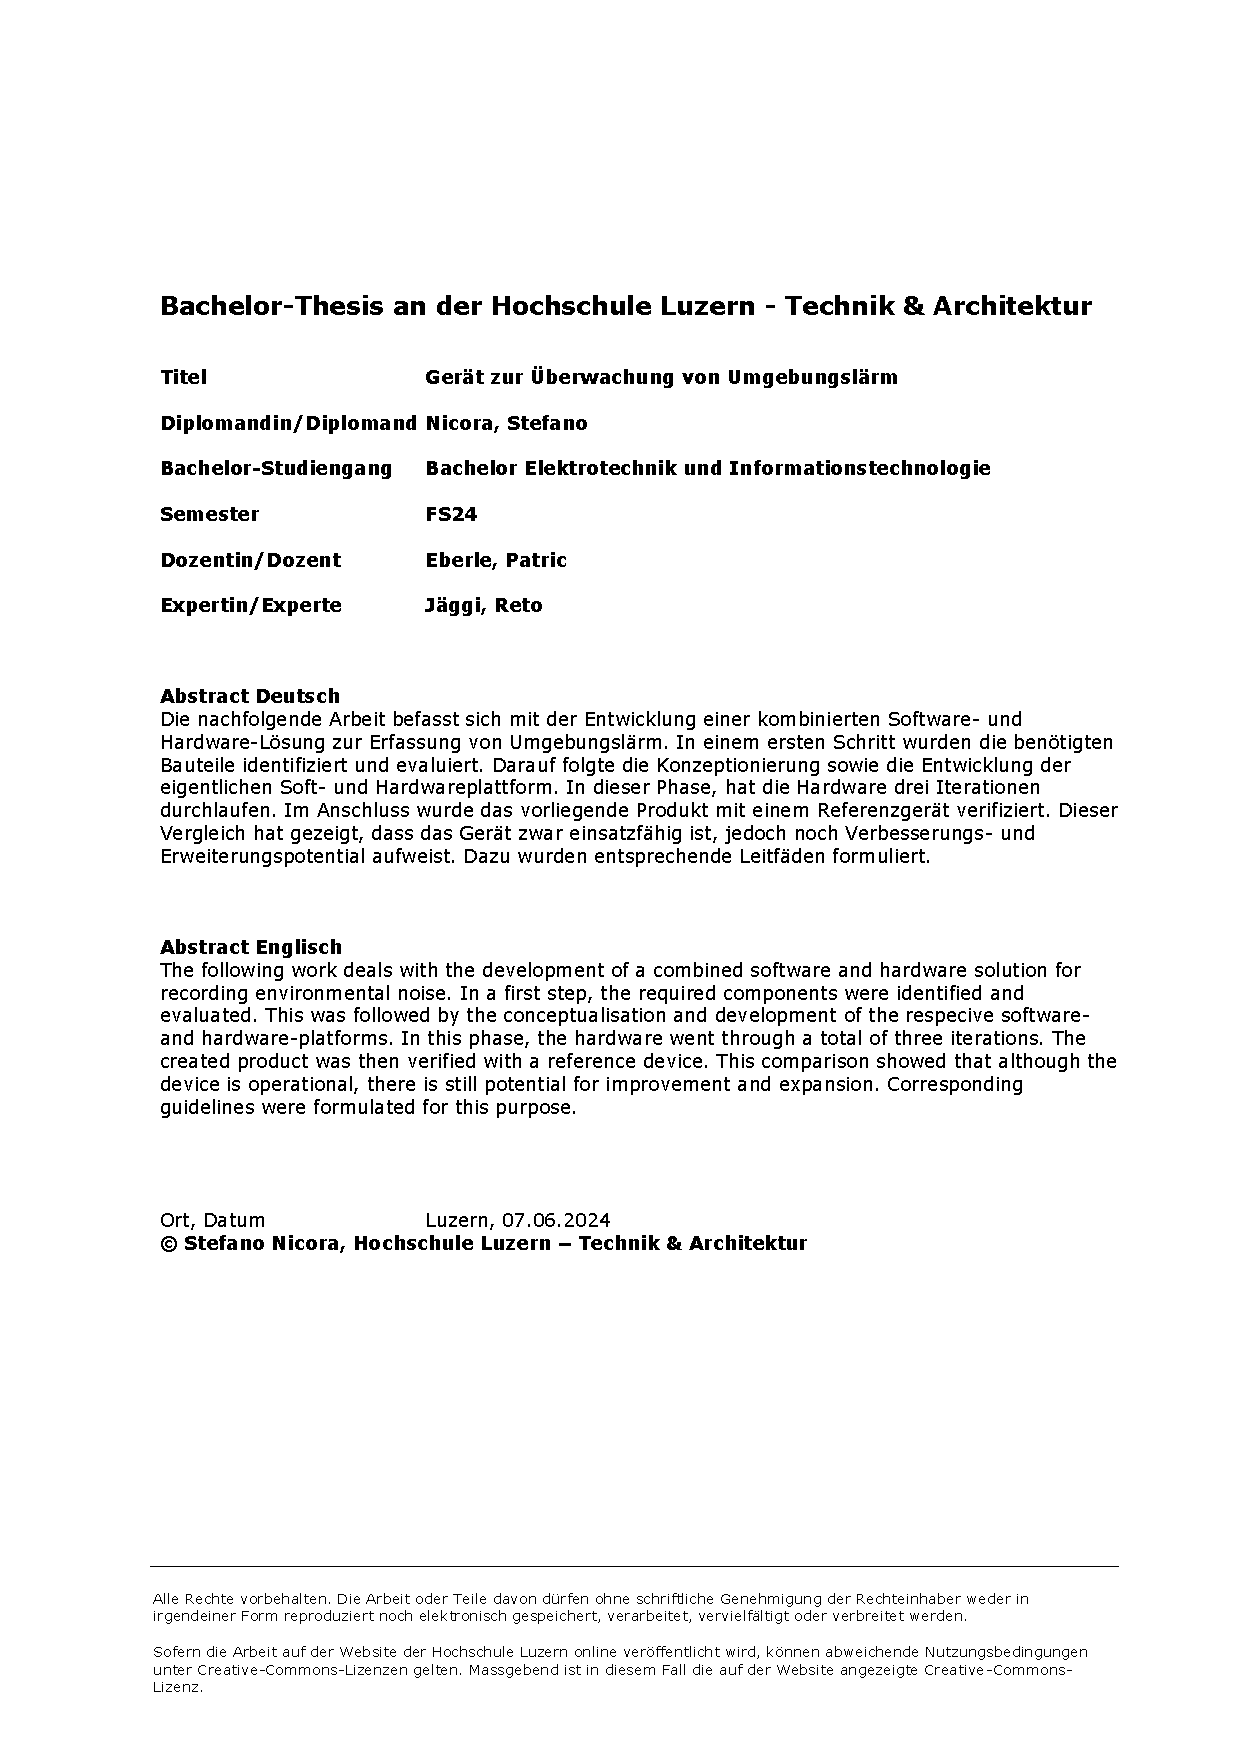
\includepdf[landscape=false, pages={1}]{delivery/BAT_Titelblatt_HSLU.pdf}
	\thispagestyle{empty}
	\tableofcontents
	\thispagestyle{empty}
	
	\newpage
	\section{Einleitung}
	Das nachfolgende Kapitel befasst sich mit den Grundanforderungen des Projektes. Unter anderem, welche Ziele erreicht werden sollen und wie sieht das gesamtheitliche Vorgehen aus.
	\setcounter{page}{1} % Set the page number to 3
	\pagestyle{plain} % Enable page numbering
	\subsection{Ausgangslage} \label{Ausgangslage}
	Die Firma hEar hat es sich zum Ziel gesetzt, gegen die für unsere Ohren schädliche Lärmbelästigung, vorzugehen. Dazu wurde in der Masterarbeit von Sophie Mia Willener eine konzeptionelle Idee für ein Messgerät ausgearbeitet. Zusätzlich dazu wurde eine Marktanalyse durchgeführt sowie ein erster Prototyp gebaut. Dieser ist jedoch noch unhandlich, nicht verifiziert und somit nicht für den Massenmarkt geeignet. An diesen Prototypen knüpft nun die nachfolgende Bachelorarbeit an und versucht die formulierten Ziele umzusetzen.
	\subsection{Ziele} \label{Ziele}
	In Übereinstimmung mit der geschilderten Ausgangslage, beabsichtigt diese Arbeit in einem ersten Schritt, auf Basis des vorhandenen Prototypen, ein funktionales, kompaktes und portables Schalldruckpegel-Messgerät zu entwickeln. Dabei sollen folgende Rahmenbedingungen zwingend eingehalten werden:
	\begin{itemize}
		\item Die Laufzeit des Gerätes soll mindestens 12 Stunden betragen.
		\item Das Gerät wird mit einem Akku betrieben. Dieser wird via eines USB-C-Anschlusses aufgeladen.
		\item Der Schalldruckpegel wird mit einem MEMS-Mikrofon aufgezeichnet.
		\item Die Messdaten werden in regelmässigen Abständen auf dem Gerät gespeichert.
		\item Das Gerät verfügt über eine BLE-Schnittstelle, um die Messdaten drahtlos an ein Zielgerät zu übertragen.
		\item Der aktuelle Schalldruckpegel wird auf der Vorderseite des Gerätes visuell dargestellt.
		\item Die Bauform der Platine fällt rund aus.
		\item Die Gesamtkosten betragen maximal 50 CHF.
	\end{itemize}
	In einem zweiten Schritt, wird das Gerät charakterisiert und dessen Qualität mit einem auf dem Markt bereits vorhandenen Gerät verglichen.
	\subsection{Vorgehen}
	Zu Projektbeginn, wurde mit hEar die zu erreichenden Ziele der Arbeit ausgearbeitet. Auf Basis dessen wurde der Anforderungskatalog (vgl. Anhang \ref{Anhang:Anforderungskatalog}) erstellt. Dieser ermöglichte es anschliessend, eine umfangreiche Risikoanalyse (vgl. Anhang \ref{Anhang:Risikoanalyse}) sowie einen geeigneten Zeitplan (vgl. Anhang \ref{Anhang:Zeitplan})zu erstellen. Nach der initialen Projektphase wurden die nötigen Grundlagen für Mikrofone (\ref{Mikrofon}), LEDs (\ref{LED}) sowie Mikrocontroller (\ref{Mikrocontroller}) aufgearbeitet und mit dem aktuellen Stand der Technik (\ref{Stand}) abgeglichen. Anschliessend folgte die Wahl der benötigten Bauteile sowie die eigentliche Hardware- und Softwareentwicklung (\ref{Entwicklung}). Nach der agilen Entwicklung folgte zum Schluss die Verifizierung mit den dazugehörigen Messungen (\ref{Messungen}) und die daraus abgeleiteten Schlussfolgerungen (\ref{Fazit}). \\
	
	\newpage
	\section{Stand der Technik}\label{Stand}
	Eine Vielzahl von unterschiedlichen Herstellern bietet diverse Messgeräte zur Messung des Schalldruckpegels an. Die Preise  reichen von 10 CHF für ein nicht genauer spezifiziertes Gerät von beispielsweise AliExpress bis hin zu über 3000 CHF für ein XL2 (vgl. Abbildung \ref{fig:batnti-audio-xl2-500}) von NTI Audio (inkl. M2211-Mikrofon). Gewisse Gemeinsamkeiten haben alle diese Geräte. Sie weisen eine Frequenzbandbreite von mind. 10kHz auf, verfügen über ein Display um die Messwerte anzuzeigen, fangen den Schall mittels eines Kondensator-Mikrofons auf und implementieren mindestens den dB(A)-Gewichtungsfilter \ref{Frequenzbewertung}. Diese Geräte sind jedoch alle durch ihre klobige Bauweise sowie ihr, für nichttechnisches Personal ungeeignetes Design, nicht für den Massenmarkt geeignet. Nichtsdestotrotz soll das in dieser Arbeit entwickelte Gerät den Parametern eines hochwertigen Gerätes entsprechen. Folglich wird es mit dem oben genannten XL2 verglichen. Die zentralen Parameter(\cite{noauthor_xl2_nodate}) sind die folgenden:
	\begin{itemize}[topsep=10pt,partopsep=0pt,labelwidth=5cm,align=left,itemindent=5cm]
		\item[$\bullet$ Frequenzbereich:]  5Hz - 20kHz
		\item[$\bullet$ Auflösung:]  0.1dB
		\item[$\bullet$ Max. dBSPL:]  144dBSPL
		\item[$\bullet$ Mikrofontyp:]  Kondensator
	\end{itemize}
	\begin{figure}[H]
		\centering
		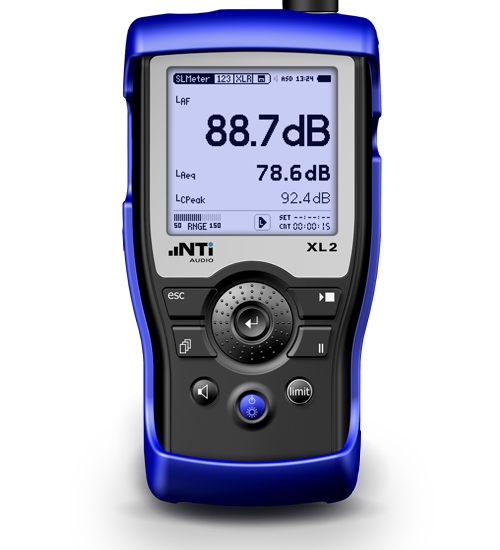
\includegraphics[width=0.4\linewidth]{images/BAT_NTi-Audio-XL2-500}
		\caption{XL2 von NTI Audio $\vert$ Quelle: \cite{noauthor_xl2_nodate}}
		\label{fig:batnti-audio-xl2-500}
	\end{figure}
		
	\newpage
	\section{Mikrofon}\label{Mikrofon}
	Als erste Kernkomponente gilt es, ein geeignetes Mikrofon zu evaluieren. Ein ungeeignetes Mikrofon entscheidet darüber, ob das Endprodukt seinen Zweck erfüllt oder nicht. Aus diesem Grund folgen anschliessend die benötigen Grundlagen, sowie die Komponentenwahl.
	\subsection{Grundlagen}
	\subsubsection*{MEMS}
	\textbf{M}icro \textbf{E}lectro-\textbf{M}echanical \textbf{S}ystems bezeichnet Bauteile, welche eine Strukturgrösse von wenigen $\mu m$ aufweisen. Aus diesem Grund werden MEMS auf Basis von Halbleitern hergestellt. Beispiele dafür sind Gyroskope (\ref{fig:batbeispielbeschleunigungssensor}), Drucksensoren, Oszillatoren oder eben Mikrofone. Bedingt durch die Strukturgrösse können kleinere Kräfte oder Drücke zuverlässiger detektiert werden. Bei Mikrofonen wird zusätzlich zwischen top- und bottom-port unterschieden (\ref{fig:batmems-mikrofon}), wobei je nach PCB-Layout nicht beide Varianten verwendet werden können. 
	\begin{figure}[H]
		\centering
		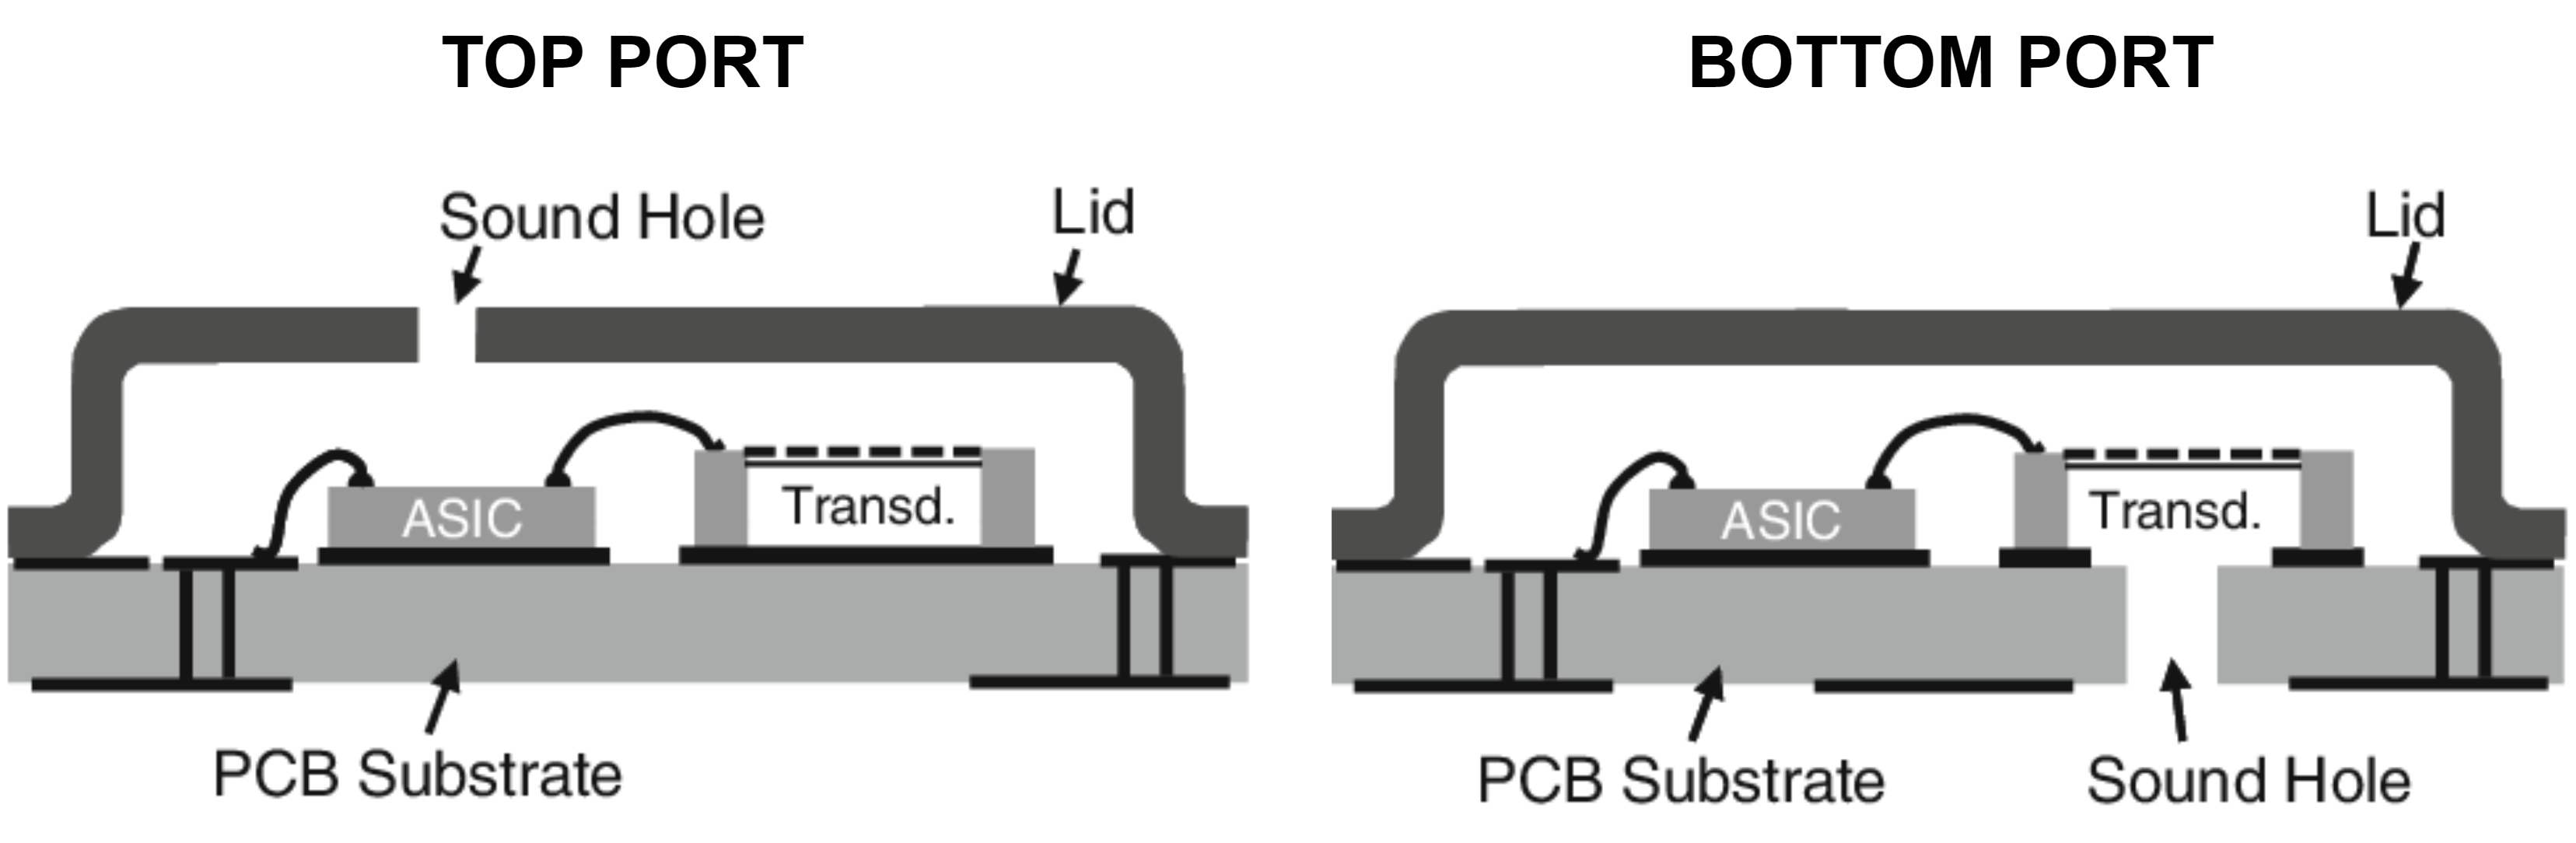
\includegraphics[width=0.6\linewidth]{images/BAT_MEMS-Mikrofon}
		\caption{Unterschied MEMS-Mikrofone $\vert$ Quelle: \cite{feiertag_flip_2010}}
		\label{fig:batmems-mikrofon}
	\end{figure}
	\begin{figure}[H]
		\centering
		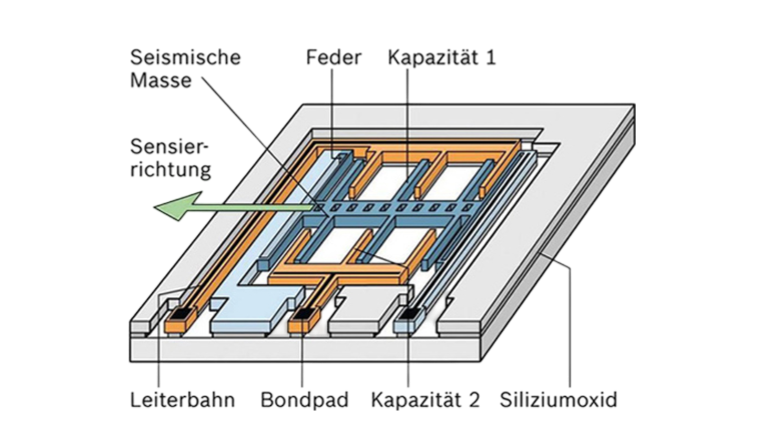
\includegraphics[width=0.55\linewidth]{images/BAT_Beispiel_Beschleunigungssensor_transparent}
		\caption{Beispiel MEMS-Beschleunigungssensor $\vert$ Quelle: \cite{noauthor_peripherer_nodate}}
		\label{fig:batbeispielbeschleunigungssensor}
	\end{figure}
	
	
	\subsubsection*{I2S} \label{I2S}
	\textbf{I}nter-\textbf{I}ntegrated \textbf{S}ound (I²S) bezeichnet eine Bus-Schnittstelle, welche von Philips zur Übertragung von digitalen Audiosignalen entwickelt wurde. Ähnlich wie I²C (Inter-Integrated Circuit) wird die Schnittstelle jedoch nur innerhalb des Gerätes verwendet. Dabei werden drei Pins zwischen Sender (hier das Mikrofon) und dem Empfänger (hier der Mikrocontroller) benötigt:
	\begin{itemize}
		\item \textbf{SCK} \quad (Serial Clock) \\
		Generiert die Taktrate, welche gleichzeitig die Datenrate der Übertragung definiert. Die Taktrate wird vom Master, hier der Mikrocontroller,  vorgegeben.
		\item \color{green}\textbf{WS}\color{black} \quad (Word Select) \\
		Gibt vor, welcher Audiokanal (R, L) übertragen werden soll. Dies ermöglicht es, entweder ein Stereo-Signal oder zwei Mono-Signale, wie zum Beispiel zwei unabhängige Mikrofone, zu übertragen.
		\item \color{red}\textbf{SD}\color{black} \quad (Serial Data) \\
		Beinhaltet den eigentlichen Datenstream mit der Datenrate, definiert durch \textbf{SCK}, und der Länge, definiert durch \color{green}\textbf{WS}\color{black}.
	\end{itemize}
	\begin{figure}[H]
		\centering
		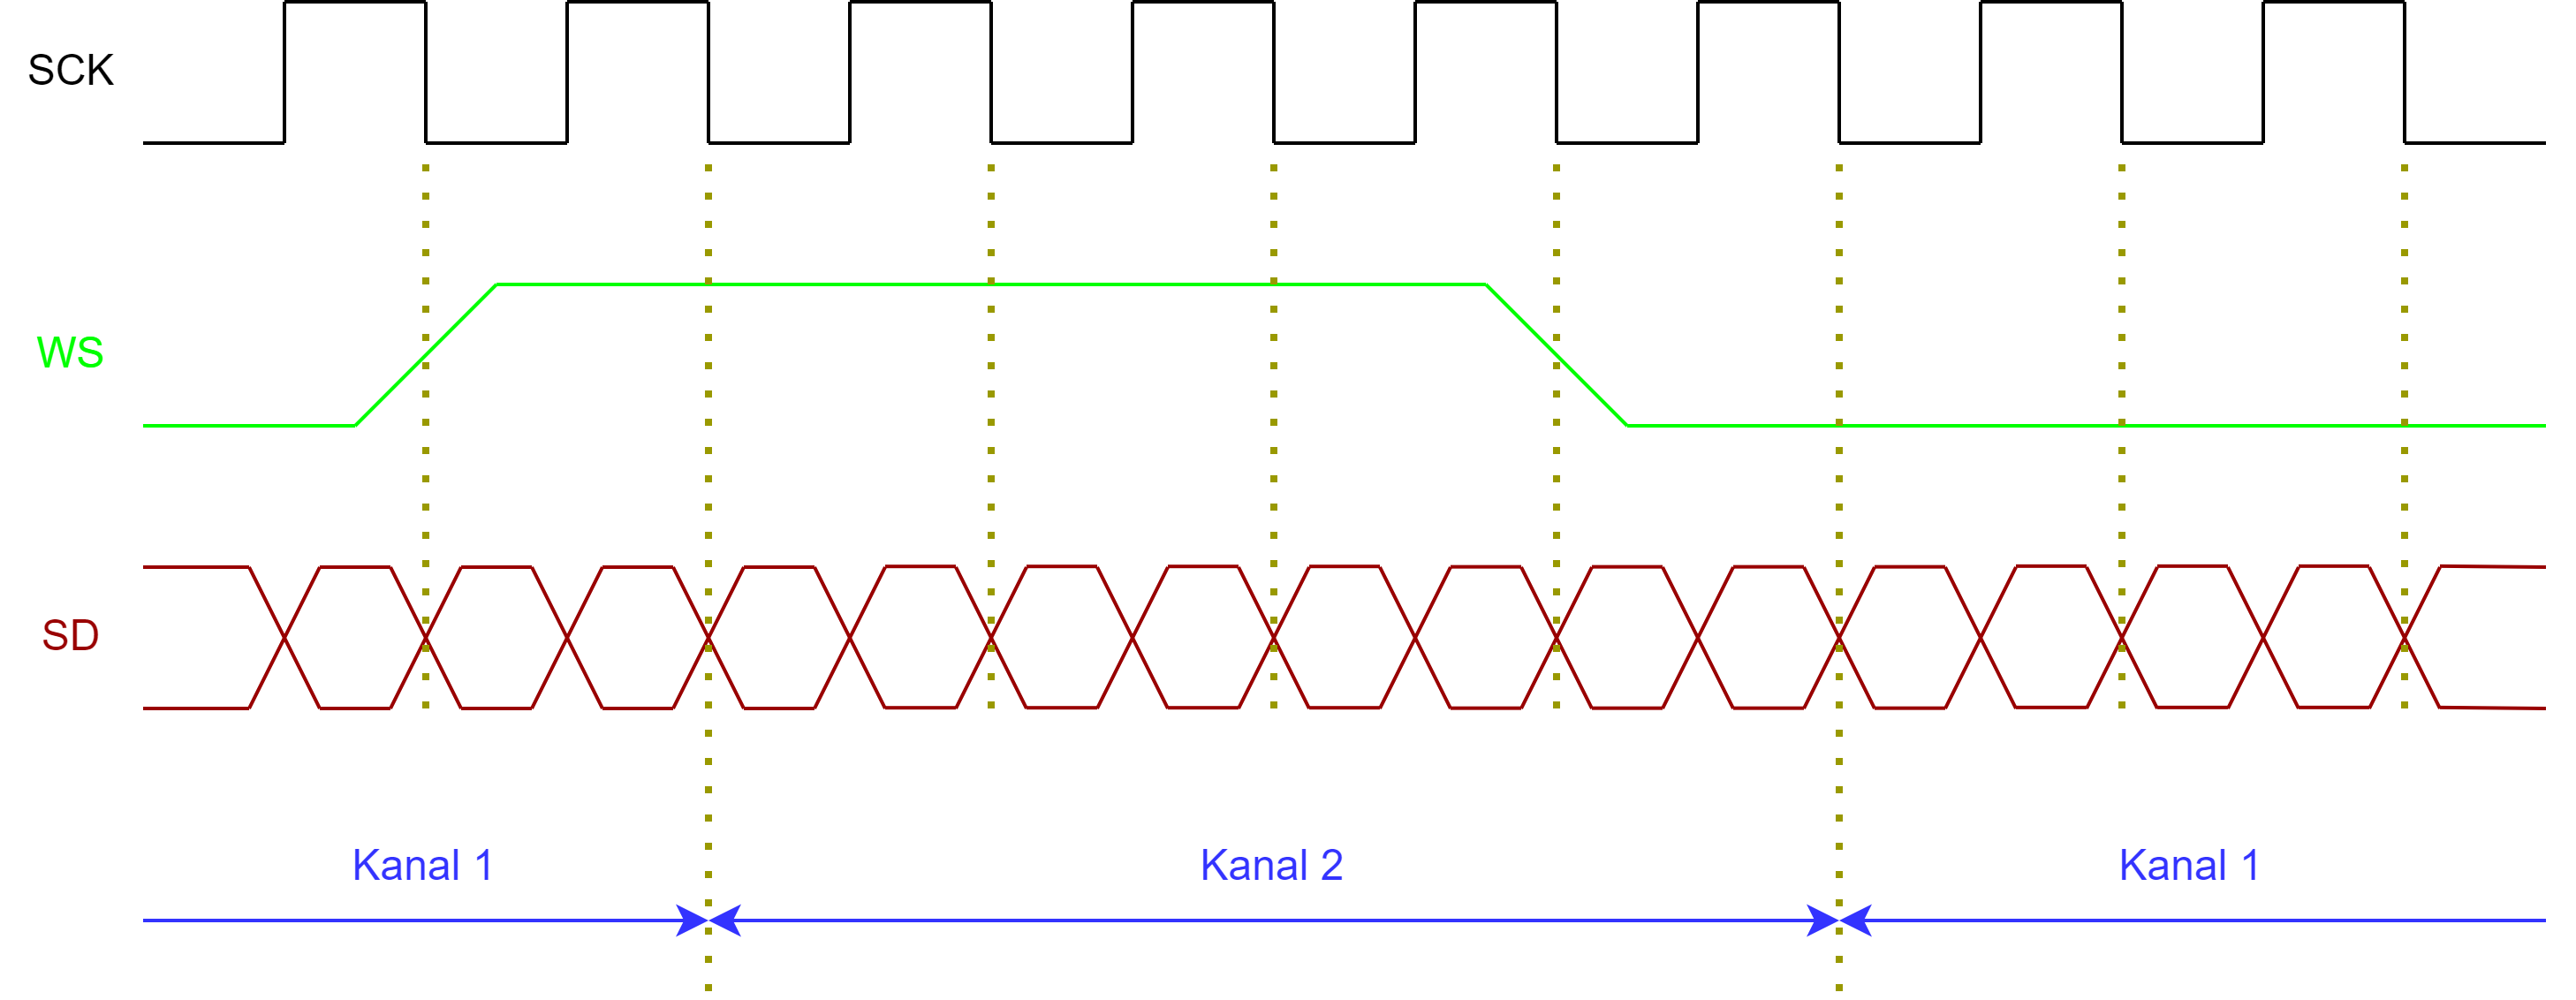
\includegraphics[width=1\linewidth]{images/BAT_I2S}
		\caption[]{Übersicht I2S-Signale}
		\label{fig:bati2s}
	\end{figure}
	\newpage
	\subsubsection*{PDM} \label{PDM}
	\textbf{P}ulse \textbf{D}ensity \textbf{M}odulation oder Pulsdichtemodulation bezeichnet die Darstellung eines analogen Signals in der digitalen Ebene. Dabei entspricht das Verhältnis zwischen der Anzahl der digitalen "1" und digitalen "0" der Amplitude des analogen Signales. Das PDM-Signal weist eine vielfach schnellere Takrate (meist Faktor 32 / 64) als das zu verarbeitende Mikrofonsignal auf. Dadurch wird auftretendes Rauschen in einen höher gelegenen Frequenzbereich verschoben, welcher bei der anschliessenden Signalverarbeitung mit einem Tiefpassfilter abgeschnitten wird. Im Gegensatz zu I²S (\ref{I2S}) werden lediglich zwei Pins zwischen Mikrofon und Empfänger benötigt:
	\begin{itemize}
		\item \color{red}DAT \color{black} \quad (Data) \\
		Beinhaltet den als PDM-Codierten Datenstream.
		\item CLK \quad (Clock) \\
		Generiert die Taktrate, mit welcher die Daten übertragen werden.
	\end{itemize}
	\begin{figure}[H]
		\centering
		\begin{minipage}{.5\textwidth}
			\centering
			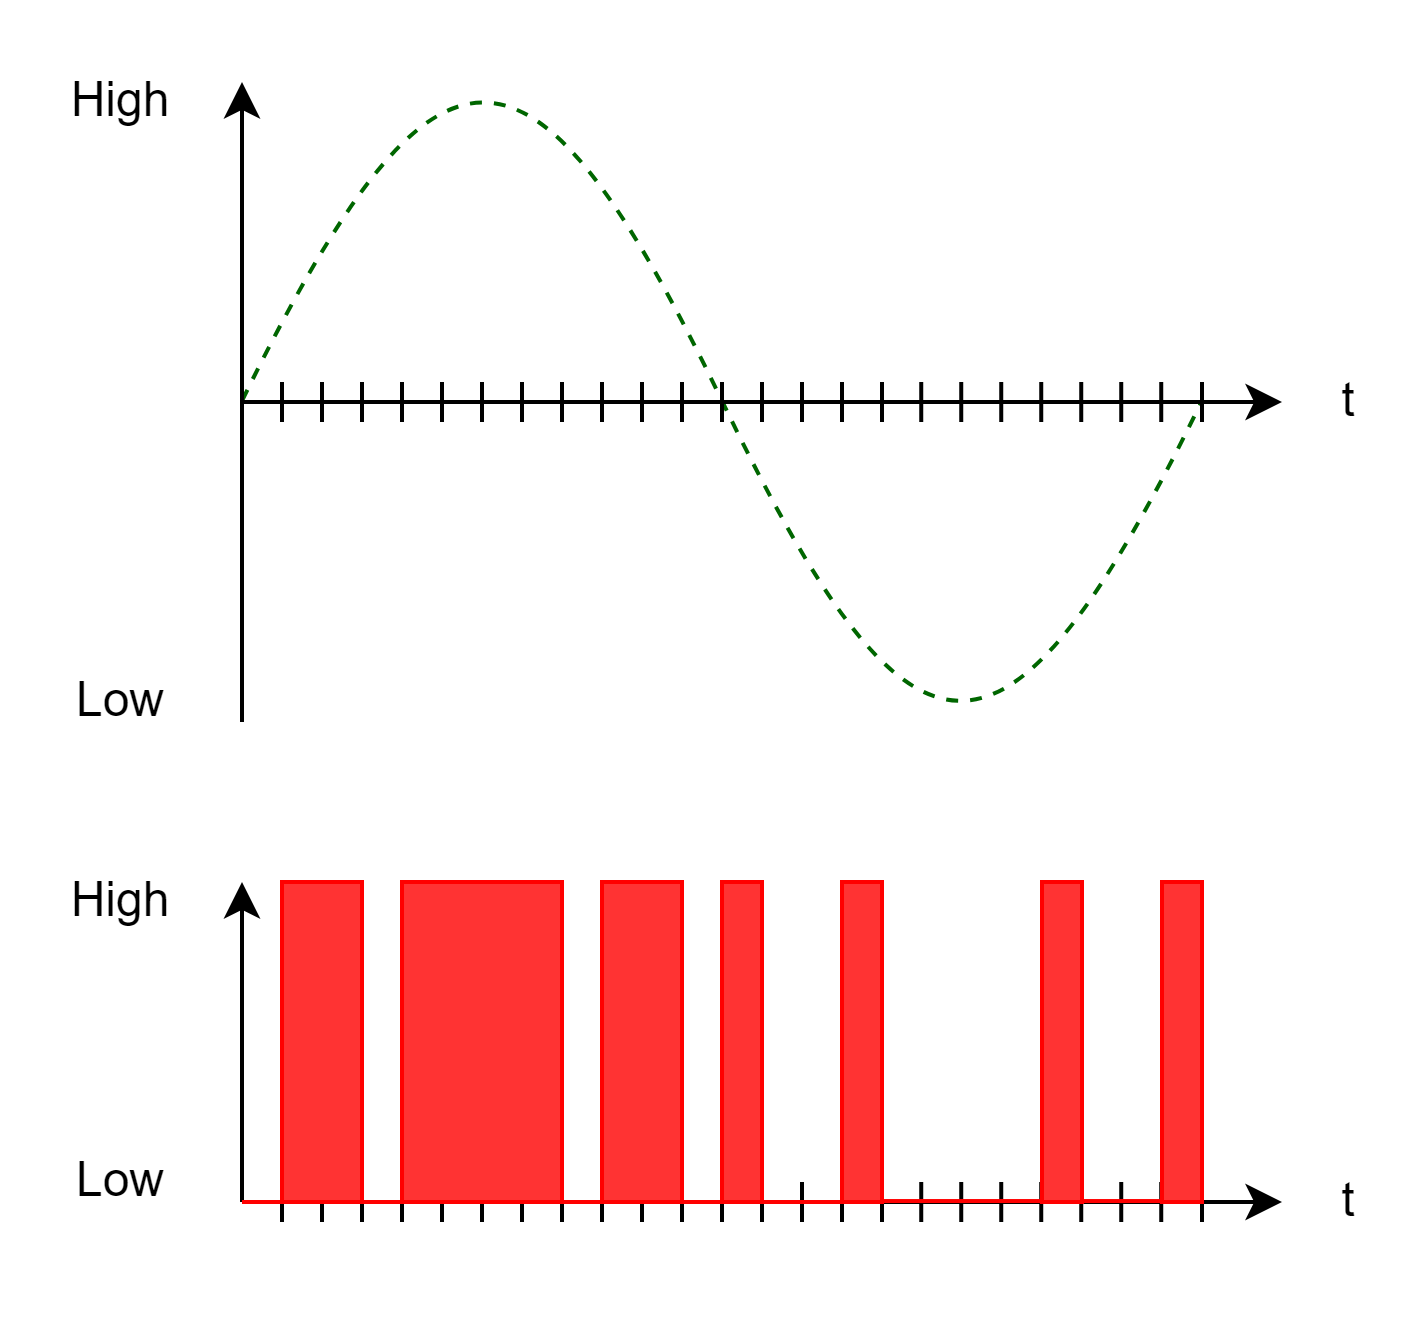
\includegraphics[width=1\linewidth]{images/BAT_PDM}
			\caption{Beispiel PDM-Signal}
			\label{fig:batpdm}
		\end{minipage}%
		\begin{minipage}{.5\textwidth}
			\centering
			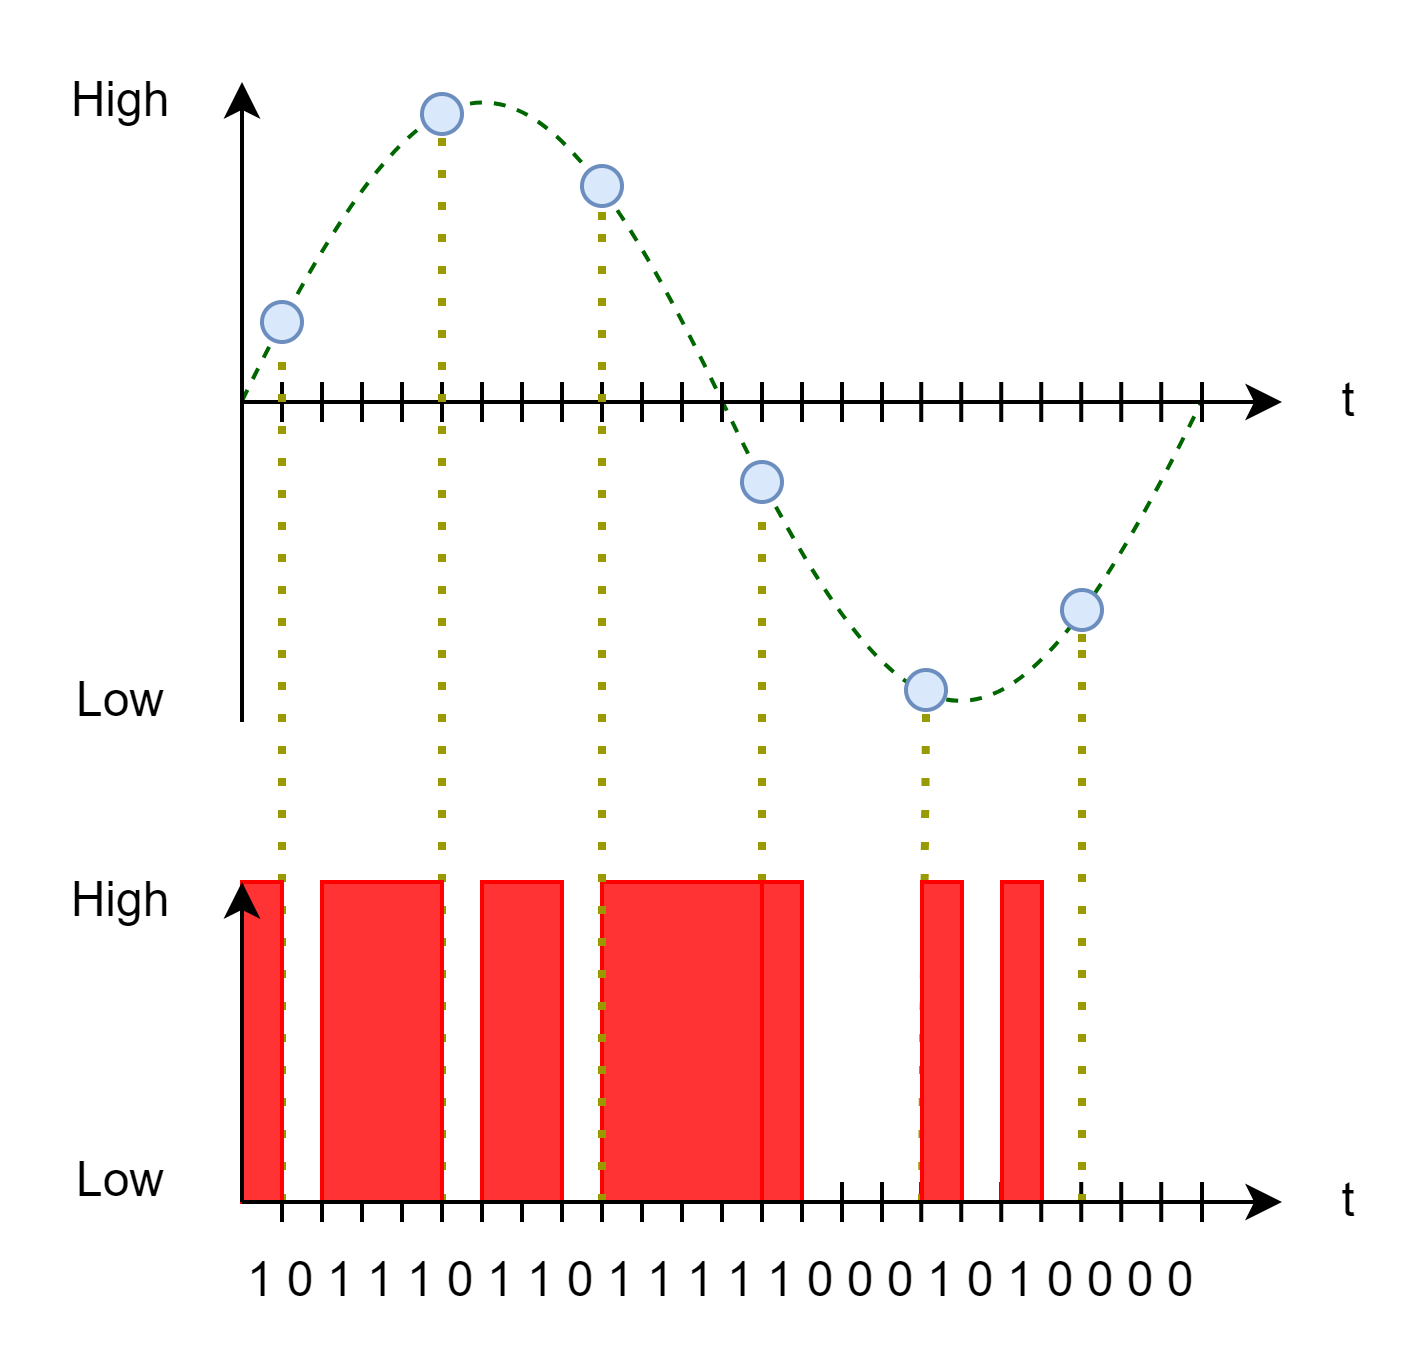
\includegraphics[width=0.97\linewidth]{images/BAT_PCM}
			\caption{Beispiel PCM-Signal}
			\label{fig:batpcm}
		\end{minipage}
	\end{figure}
	\subsubsection*{PCM}
	Bei \textbf{P}ulse \textbf{C}ode \textbf{M}odulation wird jeder analoge Messwert in einem digitalen Bereich abgebildet (Abbildung \ref{fig:batpcm}). Je nach benötigter Genauigkeit fällt dieser Bereich mal grösser, mal kleiner aus. Bei der Datenübertragung mittels I²S (\ref{I2S}) geschieht diese Umwandlung direkt im Sender und erzeugt somit das SD-Signal. Bei Sendern mit PDM-Ausgang (\ref{PDM}) ist dies nicht der Fall. Hier ist im Empfänger zwingend eine Peripherie notwendig, welche das PDM-Signal mittels Unterabtastung in ein PCM-Signal umwandelt.
	\subsubsection*{Schalldruck(pegel)}
	Damit wird der Bezug zwischen dem Schalldruck \textbf{$P$}, die Kraftauswirkung von Schallwellen auf ein Medium, und dem normierten Bezugswert \textbf{$P_0$} von $20 \mu Pa$ geschaffen. Oftmals wird der Schalldruck auch mit \textbf{S}ound \textbf{P}ressure \textbf{L}evel (SPL) angegeben. Da das menschliche Gehör Lautstärke jedoch logarithmisch wahrnimmt, wird der SPL in der Akustik mittels dBSPL (\ref{eq:dBSPL}) angegeben.
	\begin{equation}\label{eq:dBSPL}
		dB_{SPL} = 20 \cdot log_{10}(\frac{P}{P_0})
	\end{equation}
	\begin{figure}[H]
		\centering
		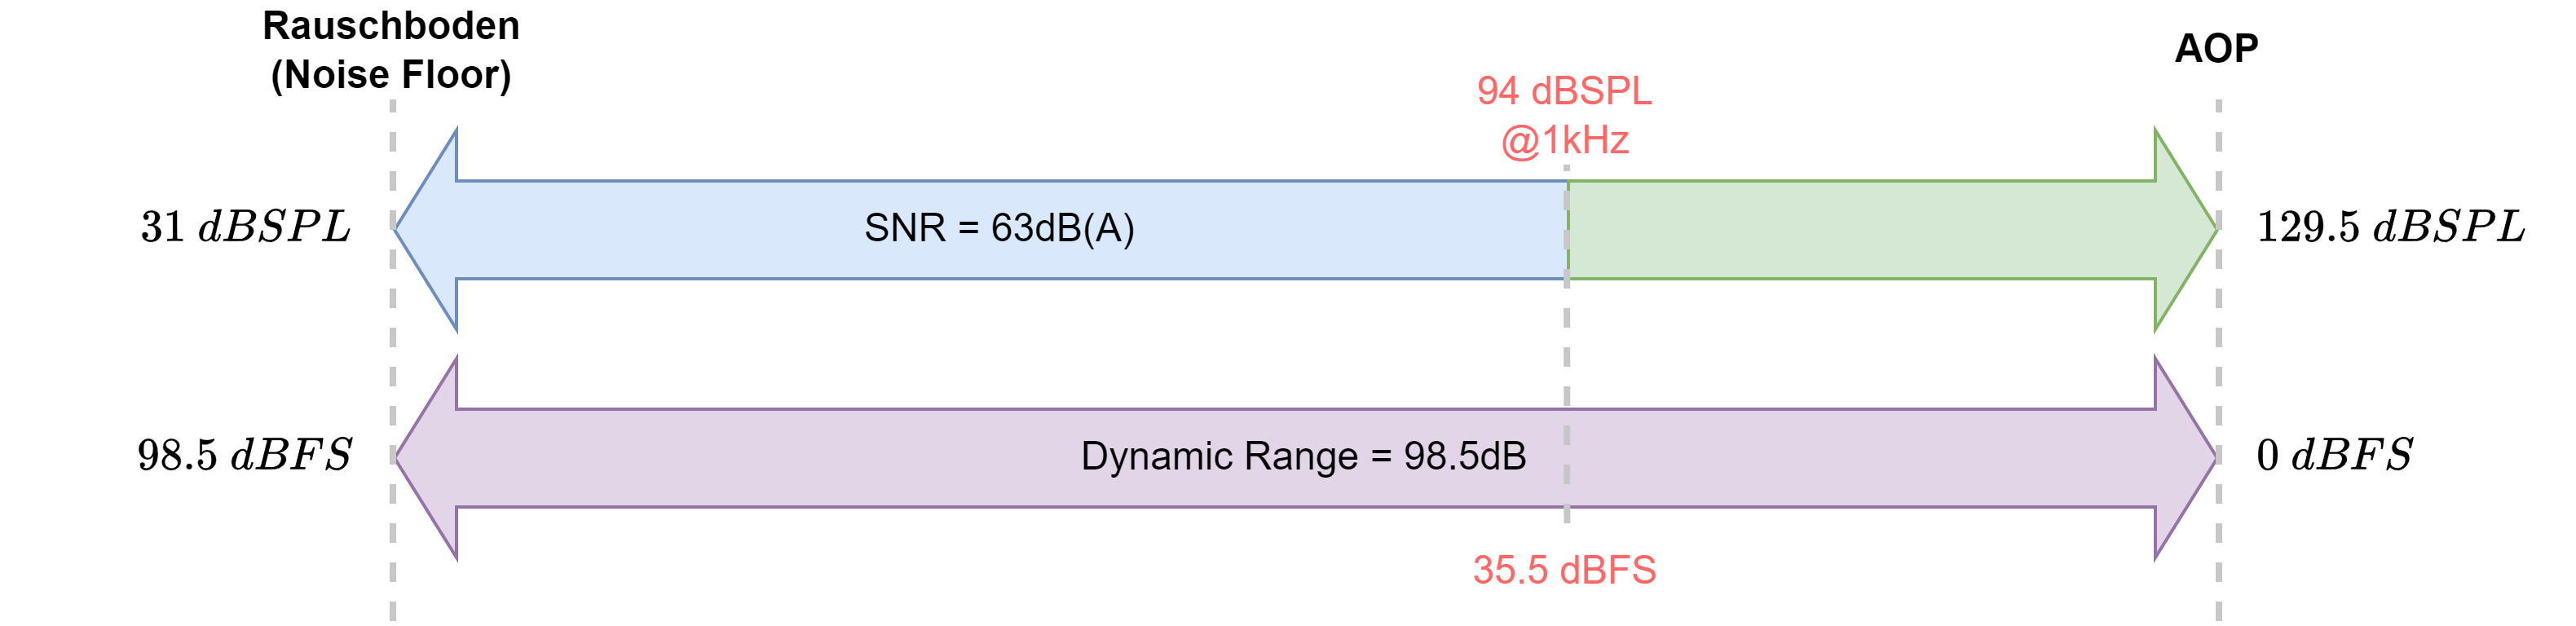
\includegraphics[width=\linewidth]{images/BAT_PDM_Grundbegriffe}
		\caption{Grundbegriffe Akustik $\vert$ Beispiel: ICS-41351}
		\label{fig:batpdmgrundbegriffe}
	\end{figure}
	\subsubsection*{AOP} \label{AOP}
	Der \textbf{A}coustic \textbf{O}verload \textbf{P}oint bezeichnet den durch ein Mikrofon maximal messbaren SPL, ohne dass es dabei zu einem Klirrfaktor (THD) von mehr als 10\% kommt. Dieser ist insbesondere dann wichtig, wenn Messungen in lauten Umgebungen vorgenommen werden müssen.
	\subsubsection*{SNR} \label{SNR}
	Der \textbf{S}ignal to \textbf{N}oise \textbf{R}atio oder Signal Rausch Abstand beschreibt die Differenz zwischen dem Referenzschalldruckpegel von 94dBSPL bei 1kHz und dem Rauschboden. Je höher diese Distanz, desto leisere Signale können noch rauschfrei gemessen werden.
	\subsubsection*{Rauschboden} \label{Rauschboden}
	Dieser bezeichnet den kleinstmöglich noch messbaren Wert, welcher nicht im Grundrauschen untergeht. Er ist vom \hyperref[SNR]{SNR} des Mikrofons abhängig.
	\subsubsection*{Dynamikbereich} \label{Dynamikbereich}
	Mit dem Dynamikbereich \ref{fig:batpdmgrundbegriffe} wird der maximal messbare Schalldruck-Unterschied bezeichnet. Dieser wird folgendermassen berechnet:
	\begin{equation}\label{mat_Dynamikbereich}
		Dynamic Range (DR) = \underbrace{dBFS_{@1kHz}}_{Datenblatt \cite{noauthor_httpsinvensensetdkcomwp-contentuploads202007ds-000157-ics-41351-v14pdf_nodate}} + \underbrace{SNR}_{Datenblatt \cite{noauthor_httpsinvensensetdkcomwp-contentuploads202007ds-000157-ics-41351-v14pdf_nodate}}
	\end{equation}
	\subsubsection*{Signalauflösung} \label{Signalauflösung}
	\begin{figure}[H]
		\centering
		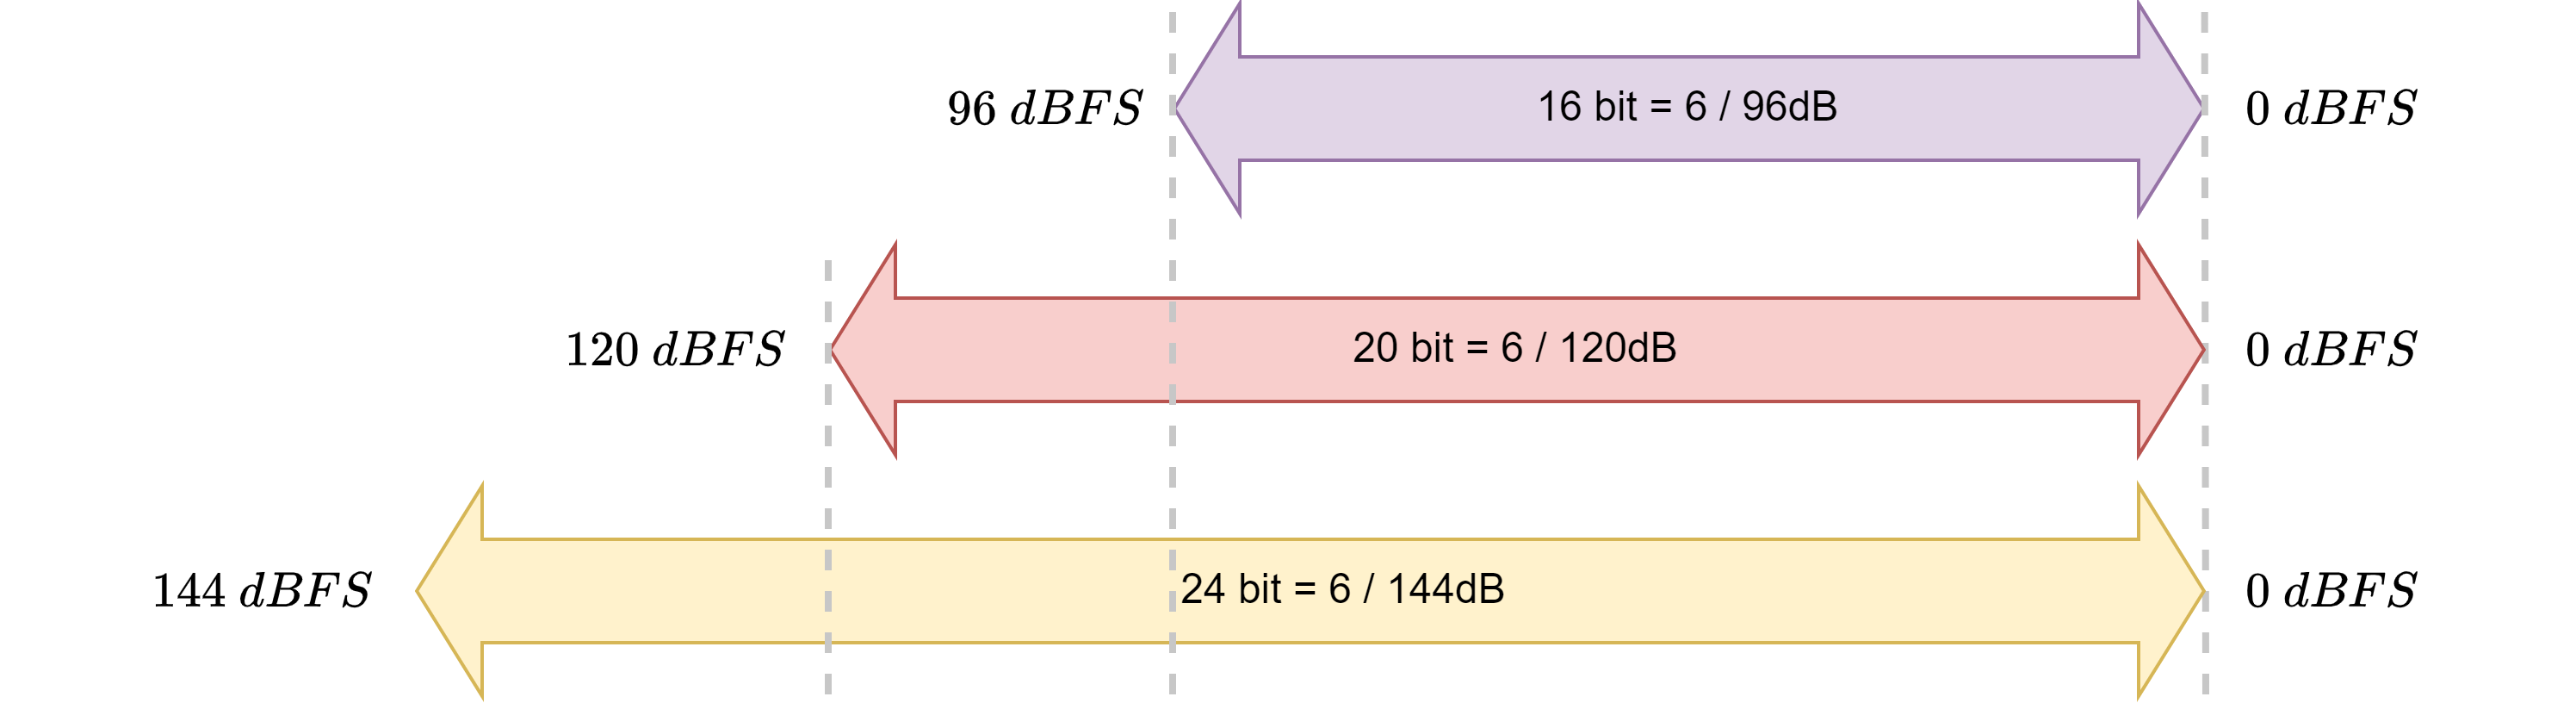
\includegraphics[width=\linewidth]{images/BAT_PDM_Codierung}
		\caption{Mind. benötigte Auflösung in Bit für gewünschten max. SPL}
		\label{fig:batpdmcodierung}
	\end{figure}
	
	\subsubsection*{Zeitgewichtung} \label{Zeitgewichtung}
	Die Zeitgewichtung wird mit dem Standard IEC 61672-1 beschrieben und definiert, wie schnell die Anzeige des Gerätes auf eine Pegeländerung reagieren kann. Dabei wird gemäss Abbildung \ref{fig:batf-s-time-weighting} zwischen den Modi \textbf{S}low und \textbf{F}ast unterschieden. Die Modi stammen aus der Zeit der analogen Anzeigesysteme, wobei schnelle Änderungen der Anzeige nur schwer ablesbar sind. Implementationstechnisch werden neuere Messwerte stärker gewichtet, als die alten um auf kurzzeitige Amplitudenänderungen besser reagieren zu können.
	\begin{figure}[H]
		\centering
		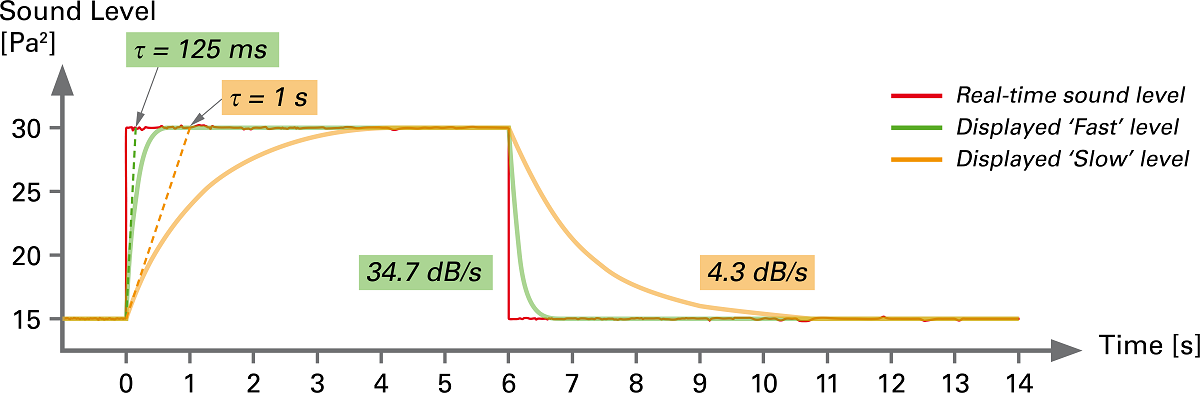
\includegraphics[width=1\linewidth]{images/BAT_F-S-time-weighting}
		\caption{Unterschied der Zeitgewichtung $\vert$ Quelle: \cite{noauthor_was_nodate}}
		\label{fig:batf-s-time-weighting}
	\end{figure}
	
	\subsubsection*{Frequenzbewertung} \label{Frequenzbewertung}
	Unser Gehör reagiert zum einen nichtlinear auf Lautstärkeveränderungen, zum anderen auch unterschiedlich sensitiv auf unterschiedliche Frequenzen im hörbaren Bereich (20Hz-20kHz). Insbesondere im Frequenzbereich zwischen 3kHz bis 4kHz \cite{impairments_basics_2004} ist das Gehör besonders anfällig auf äussere Stimulationen. Abbildung \ref{fig:phon-curve}, ursprünglich durch Fletcher \& Munson, mittlerweilen auch durch den ISO226-Standard beschrieben, zeigt diesen Umstand. Um der Problematik aus Abbildung \ref{fig:phon-curve} Sorge tragen zu können, wird ein sogenannter Frequenzbewertungsfilter \footnote{ Weighting curves}, Abbildung \ref{fig:frequenzbewertung}, eingesetzt. Dabei werden heutzutage nur noch die dB(A), sowie der dB(C)-Filter eingesetzt. Die beiden Filter unterscheiden sich folgendermassen:
	\begin{itemize}
		\item dB(A) \\
		Reproduziert die 40 Phon Kurve \\
		Widerspiegelt das menschliche Gehör besser als der dB(C)-Filter
		\item dB(C) \\
		Reproduziert die 100 Phon Kurve.\\
		Filtert weniger tiefe und hohe Frequenzen als dB(A) heraus\\
		Wird zur Messung in besonders lauter Umgebung eingesetzt
	\end{itemize}
	\begin{figure}[H]
		\centering
		\begin{minipage}{.5\textwidth}
			\centering
			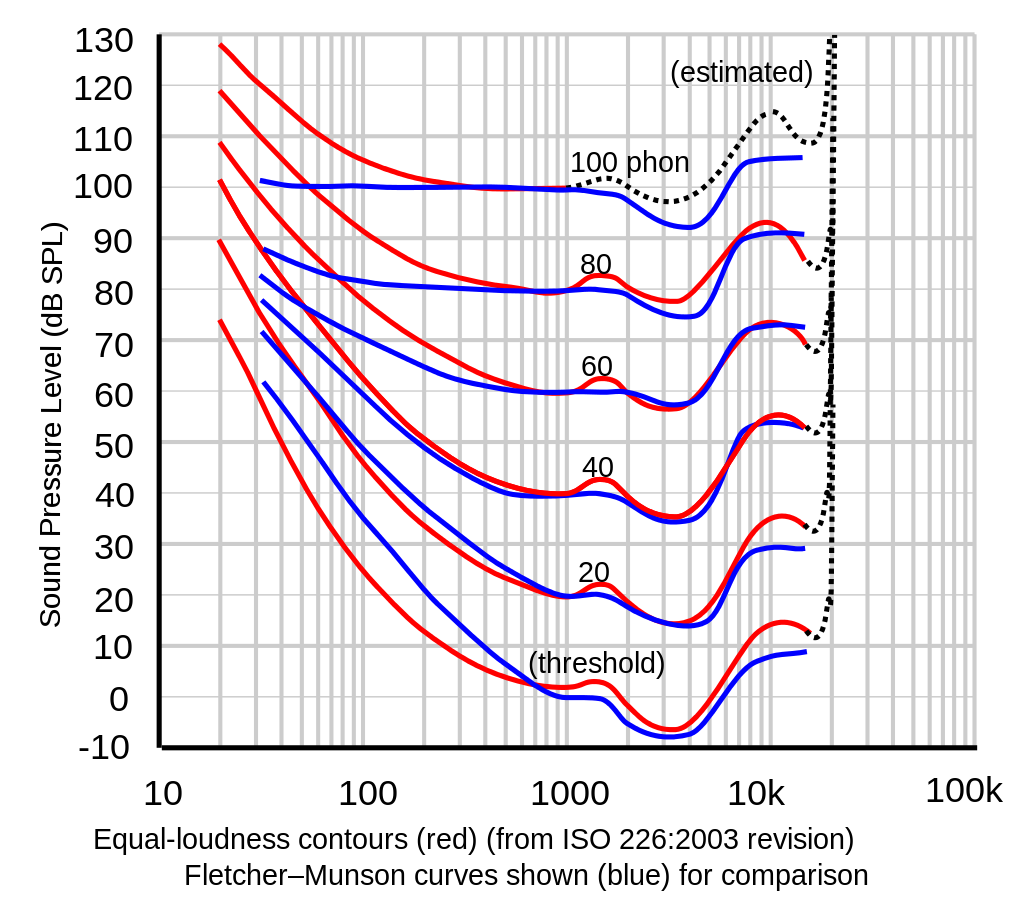
\includegraphics[width=1\linewidth]{images/phon-curve}
			\caption{Phon-Kurven im \\ Vergleich $\vert$ Quelle: \cite{impairments_basics_2004}}
			\label{fig:phon-curve}
		\end{minipage}%
		\begin{minipage}{.5\textwidth}
			\centering
			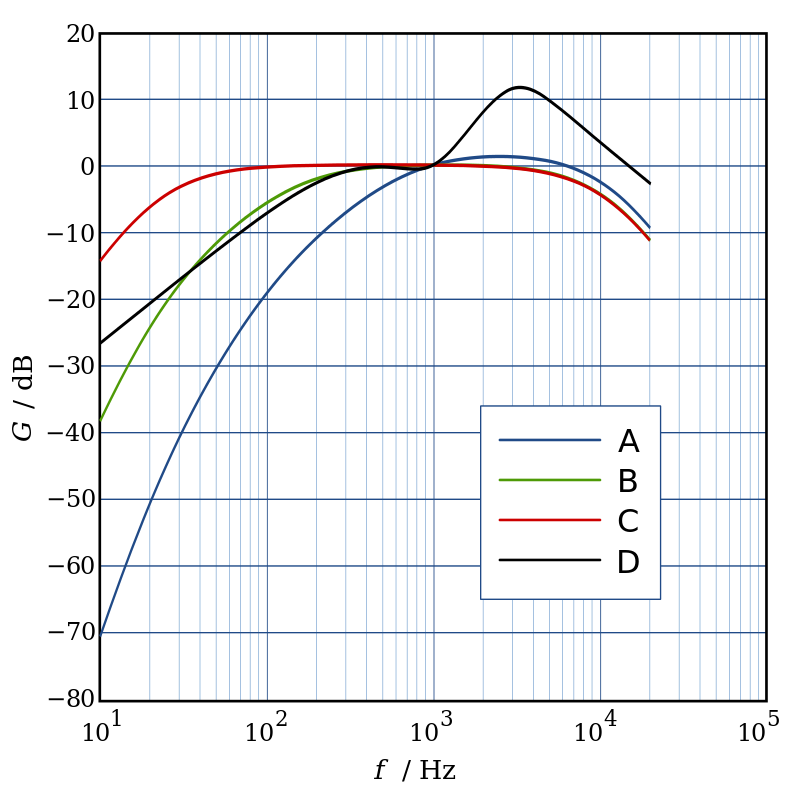
\includegraphics[width=0.9\linewidth]{images/Frequenzbewertung}
			\caption{Frequenzbewertungs\-filter $\vert$ Quelle: \cite{noauthor_frequenzbewertung_2023}}
			\label{fig:frequenzbewertung}
		\end{minipage}
	\end{figure}
	
	\subsection{Komponentenwahl}
	Wie den Anforderungen, sowie den Grundlagen zu entnehmen ist, müssen für die Wahl des besten Mikrofons gewisse Kritierien berücksichtigt werden.
	\subsubsection{Kriterien}
	\begin{itemize}
		\item Standort der Mikrofon-Öffnung
		\item Ausgangssignal
		\item Maximaler Schalldruckpegel
		\item MEMS-Technologie
		\item Frequenzbereich
	\end{itemize}
	\subsubsection{Vergleich}
	\begin{table}[H]
		\centering
		\begin{tabular}{|p{0.2\textwidth}|l|l|l|l|l|l|}
			\hline
			\textbf{Typ} & \textbf{Data} & \textbf{Öffnung} & \textbf{\hyperref[SNR]{SNR}[dB]} & \textbf{\hyperref[AOP]{AOP}[dB]} & \textbf{$f_{min}$[Hz]} & \textbf{$f_{max}$[Hz]} \\\hline
	ICS-43434 & I2S & unten & 65 & 120 & 60 & 20000 \\ \hline
	ICS-41351 & PDM & oben & 65 & 129.5 & 50 & 20000 \\ \hline
	MMICT5838-00-012 & PDM & unten & 68 & 133 & 27 & 20000 \\ \hline
	CMM-4737DT-26386-TR & PDM & oben & 58 & 120 & 100 & 10000 \\ \hline
	CMM-4737DT-26186-TR & PDM & oben & 58 & 120 & 100 & 10000 \\ \hline
	MP34DT05(-A) & PDM & oben & 64 & 122.5 & 100 & 10000 \\ \hline
	MP34DT06J & PDM & oben & 64 & 122.5 & 100 & 10000 \\ \hline
	SPH0645LM4H-B & I2S & unten & 65 & 120 & 20 & 10000 \\ \hline
	\end{tabular}
	\caption{Vergleich Mikrofone}
	\label{table:vergleich-mikrofone}
\end{table}

	\subsubsection{Fazit}
	Ein Drittel der untersuchten Mikrofone haben die Mikrofon-Öffnung auf der Unterseite. Dies ermöglicht es, einen höheren SNR gewährleisten zu können, jedoch ist diese Montageart für das Endprodukt nicht geeignet (vgl. Kapitel \ref{Entwicklung}). Bei den restlichen Mikrofonen sticht das ICS-41351 von TDK InvenSense mit seinem hohen SNR, AOP sowie der hohen Frequenzbandbreite heraus.
	
	\newpage
	\section{Mikrocontroller}\label{Mikrocontroller}
	Der Mikrocontroller repräsentiert die zweite Kernkomponente des Systems. Aus diesem Grund folgen anschliessend die benötigen Grundlagen, sowie die eigentliche Komponentenwahl.
	\subsection{Grundlagen}
	\subsubsection*{DMA}
	Bei \textbf{D}irect \textbf{M}emory \textbf{A}ccess handelt es sich um eine Art Steuerbaustein, welcher unabhängig und parallel zum eigentlichen Rechenkern arbeitet. Dieser hat, wie der Rechenkern selbst, Zugriff auf den gesamten Datenbus. Dieser ermöglicht es, effizient Daten von Peripherien wie der UART, I²S, SPI, ect. in den RAM und umgekehrt zu laden. Dadurch wird der Rechenkern entlastet und kann für wichtigere Aufgaben eingesetzt oder gar in einen Energiesparmodus versetzt werden. Dabei sind zwei Möglichkeiten vorhanden, mit dem DMA-Baustein zu interagieren:
	\begin{itemize}
		\item Bus Master \\
		Der DMA-Baustein wird einmalig durch den Rechenkern aufgesetzt und läuft danach autonom. So können beispielsweise via I²S einkommende Daten automatisch aus dem Eingangsregister in den Speicher geladen werden. Bei genügend grosser Datenmenge (definiert durch den Entwickler), kann der Rechenkern wieder aus dem Energiesparmodus aufgeweckt werden und gesammelten Daten verarbeiten.
		\item Programmed I/O \\
		Jeder Arbeitsprozess des DMA-Bausteins wird durch den Rechenkern gestartet. Da sich DMA und Rechenkern den Datenbus teilen, wird so garantiert, dass der Datentransfer zum gewünschten Zeitpunkt stattfindet.
	\end{itemize}
	\subsubsection*{Bootloader}
	Unter einem Bootloader versteht man Code, welcher grundsätzlich nach dem erstmaligen flashen persistent im System bleibt. Er dient als Ausgangspunkt für die eigentliche Software und ermöglicht es beispielsweise auch, während der Laufzeit des Gerätes Softwareupdates herunterzuladen und diese anschliessend einzuspielen. Insbesondere wenn Funkprotokolle wie Bluetooth oder WLAN eingesetzt werden, ist ein Bootloader oftmals unerlässlich. Der Nachteil ist jedoch, dass dieser den ohnehin knappen Speicherplatz weiter reduziert.
	\subsubsection*{RTC}
	Unter einer \textbf{R}eal \textbf{T}ime \textbf{C}lock versteht man ein Stück Hardware (intern oder extern), welche die Zeit ab Inbetriebnahme misst. Übliche RTCs haben, aufgrund ihrer Bauweise, eine Genauigkeit von 100ppm. Da dies einer Zeitverschiebung von 4 min und 19 s @32kHz entspricht, enthalten die meisten RTCs Kompensationsmechanismen, um diese Zeit auf unter 100 ms zu bringen. \cite{dighe_tps65950_2008}

	\subsubsection*{Low Power}
	Mit Low Power wird, insbesondere bei Embedded-Systemen, die reduzierte Energieaufnahme beschrieben. Oftmals verfügen die Systeme über mehrere Modi mit jeweils unterschiedlichen Eigenschaften. Das Ziel ist es, mit jedem tieferen Modus etwas mehr Energie zu sparen und somit die Akkulaufzeit zu verlängern. Wie in Abbildung  \ref{fig:batlow-power-modestm} ersichtlich, sinkt zwar die Energieaufnahme mit jeder Stufe, jedoch werden dabei gewisse Peripherien abgeschaltet und die allgemeine Startzeit des Systems wird erhöht.
	\begin{figure}[H]
		\centering
		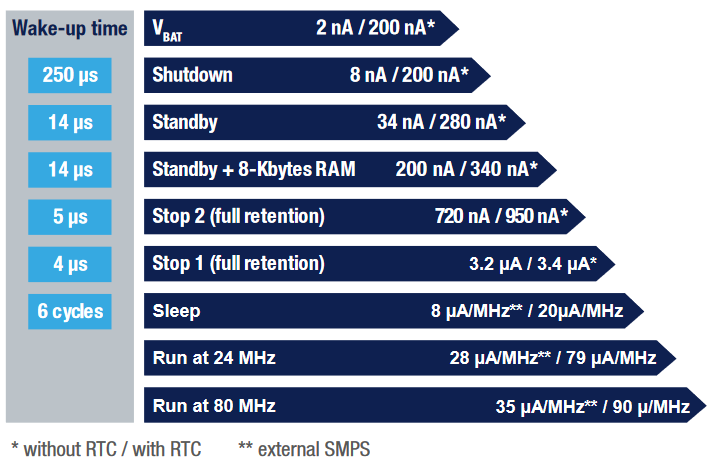
\includegraphics[width=0.7\linewidth]{images/BAT_Low-Power-Mode_STM}
		\caption{Vergleich Low-Power-Modi STM $\vert$ Quelle: \cite{noauthor_stm32l4_2024}}
		\label{fig:batlow-power-modestm}
	\end{figure}
	
	\subsubsection*{Peripherie in Hardware oder Software}
	Bei allen gängigen Kommunikationsprotokollen ist die Frage, wie diese implementiert werden sollen. Dabei stehen folgende Möglichkeiten zur Auswahl:
	\begin{itemize}
		\item in \textbf{Hardware} \\
		+ Die benötigte Infrastruktur (Register, CRC, etc.) sind bereits physika\-lisch implementiert. Die Kommunikation kann dementsprechend vom Rechenkern abgekoppelt durchgeführt werden und ermöglicht eine ge\-wisse Parallelität von mehreren Prozessen mit wenig Rechenaufwand. Insbesondere in Verbindung mit DMA kann so viel Rechenzeit eingespart werden. \\
		- Bei den meisten Mikrocontrollern ist die spezifische Hardware an einzelne Pins gebunden. Dies wirkt sich auf die Flexibilität des PCB-Layouts oder gar des Gesamtsystems (zu wenig Anschlüsse vorhanden) aus.
		\item in \textbf{Software} \\
		+ Die meisten Pins können flexibel für jedes Protokoll verwendet werden. Dadurch vereinfacht sich auch das PCB-Layout.\\
		- Bei Verwendung von Ein-Kern-Systemen, welche im Embedded-Bereich mehrheitlich anzutreffen sind, kann keine echte Parallelität von Prozessen erfolgen. Dies verringert die Ausführungsgeschwindigkeit.
	\end{itemize}
	Grundsätzlich ist, nach Möglichkeit und Verfügbarkeit, eine Hardware-Peripherie zu bevorzugen. Insbesondere bei batteriebetriebenen Systemen mit langer Laufzeit, ist diese ausschlaggebend.
	\subsection{Komponentenwahl}
	Es existieren eine Vielzahl von Mikrocontroller-Herstellern. Viele dieser verfügen über eine breite Palette an BLE-tauglichen Chips. Um den geeignetsten darunter zu finden, werden nachfolgend die benötigten Schnittstellen definiert und mehrere vorselektionierte Mikrocontroller miteinander verglichen.
	\subsubsection{Kriterien}
	\begin{itemize}
		\item \textbf{I²S} + \textbf{PDM} zur Ansteuerung des Mikrofons
		\item \textbf{SPI} zur Ansteuerung von möglichen Peripherien wie externe Speicher\-bausteine oder Displays
		\item \textbf{I²C} zur Ansteuerung von Laderegler und LED-Treiber-IC
		\item \textbf{DMA} zur energieeffizienten Verarbeitung der Daten
		\item \textbf{RTC} um die gemessenen Werten mit einem Zeitstempel verknüpfen zu können
		\item \textbf{BLE}-Fähiger Mikrocontroller mit vorgefertigter Antenne um die Integration zu vereinfachen
	\end{itemize}
	\subsubsection{Vergleich} \label{Vergleich_uC}
	\begin{figure}[H]
		\centering
		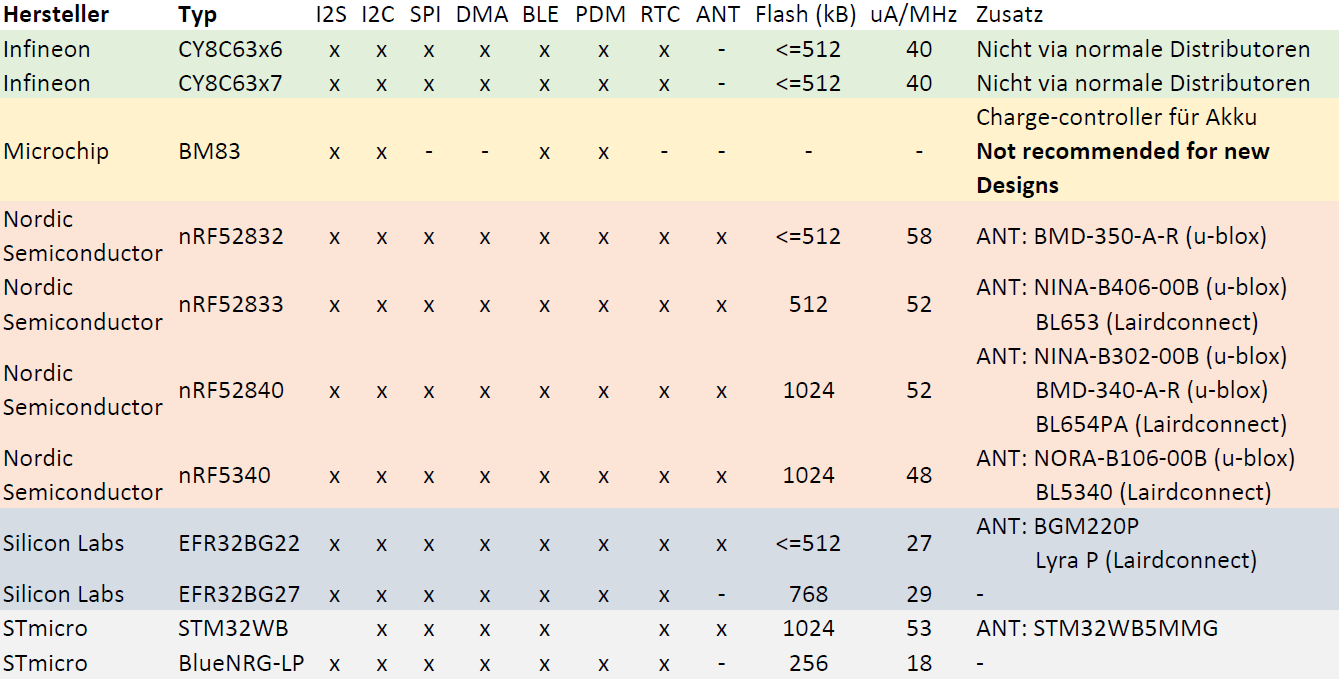
\includegraphics[trim=55 260 230 70, width=1\linewidth]{tables/BAT_Vergleich-Mikrocontroller}
		\caption{Vergleich von möglichen Mikrocontrollern}
		\label{fig:batvergleich-mikrocontroller}
	\end{figure}
	\subsubsection{Fazit}
	Wie dem \hyperref[Vergleich_uC]{Vergleich} zu entnehmen ist, unterscheiden sich die Mikrocontroller meist nur in der integrierten Flash-Grösse sowie der Energieaufnahme bei einer gewissen Taktrate. Dadurch wird die Wahl nicht eingeschränkt, was die Evaluation nicht vereinfacht. Ausschlaggebend ist jedoch der Formfaktor. Bis auf Silicon Labs und STmicro muss für einen Mikrocontroller mit vorgefertigter Antenne auf Drittanbieter ausgewichen werden. In Zeiten von Katastrophen wie COVID oder Kriegen inmitten von Handelsrouten ist die Produktverfügbarkeit einer der zentralen Aspekte. Aus diesem Grund wird nachfolgend der EFR32BG22 von Silicon Labs bzw. dessen Modul-Variante, der \textbf{BGM220P}, eingesetzt.
	
	\newpage
	\section{LED}\label{LED}
	Die visuelle Darstellung des Schalldruckpegels kann auf verschiedene Arten umgesetzt werden. Da hEar explizit eine Darstellung mittels LED wünscht, werden nachfolgend die wichtigsten Charakteristiken eingeführt und anschlie\-ssend ein passendes Produkt evaluiert.
	\subsection{Grundlagen}
	\subsubsection*{Wellenlänge} \label{Wellenlänge}
	Das für den durchschnittlichen Menschen sichtbare Lichtspektrum beginnt bei 380nm (blau) und endet bei 780nm (rot)\cite{noauthor_v-lambda-kurve_2023}. Wie der Abbildung \ref{fig:batv-lambda-curve} zu entnehmen ist, entspricht die Sensitivität einer Gausskurve. Dabei erreicht diese ihr Maximum bei 555nm (grün) bei Betrachtung der Tageskurve. Dementsprechend kann beim Einsatz einer 555nm-LED im Gegensatz zu LEDs mit einer tieferen oder höheren Wellenlänge die zugeführte Leistung bei gleichwertiger Lichtempfindlichkeit reduziert werden.
	\begin{figure}[H]
		\centering
		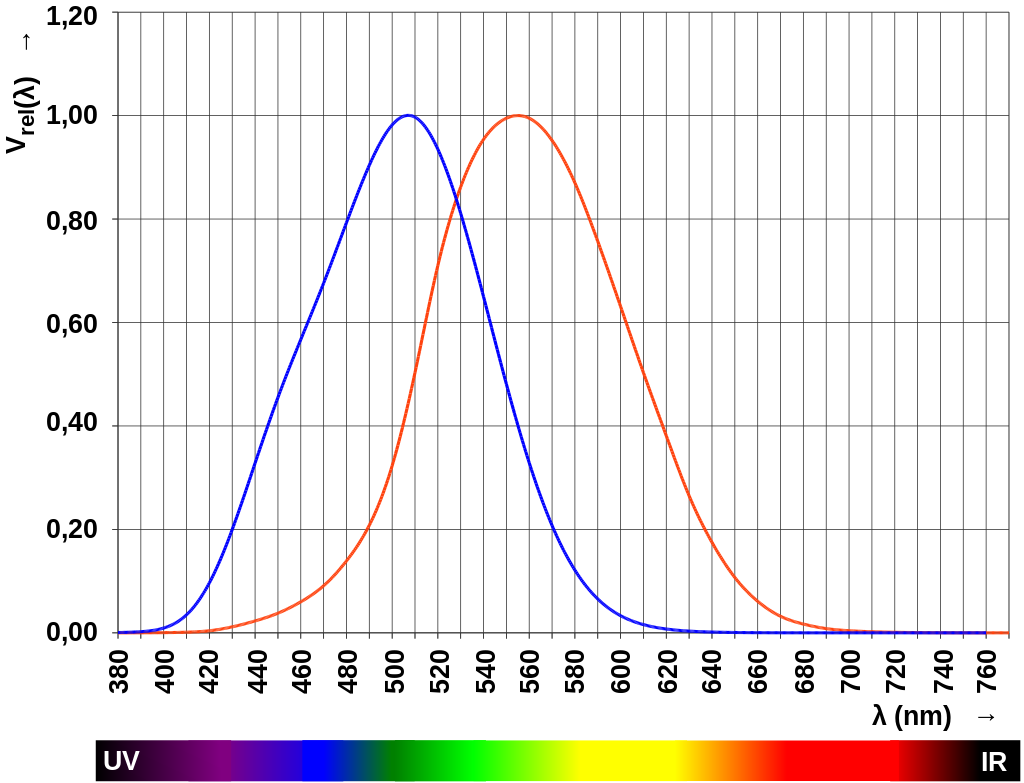
\includegraphics[width=0.8\linewidth]{images/BAT_v-lambda-curve}
		\caption{Sensitivität des menschlichen Auges auf das Lichtspektrum bei Tag (\color{red}\textbf{rot}\color{black}) und Nacht (\color{blue}\textbf{blau}\color{black})$\vert$ Quelle: \cite{noauthor_v-lambda-kurve_2023}}
		\label{fig:batv-lambda-curve}
	\end{figure}
	\subsubsection*{Lichtleistung}
	Neben der Wellenlänge ist die Lichtleistung ausschlaggebend für die wahr\-genommene Helligkeit einer LED. Dabei wird die Lichtleistung in Candela [cd] angegeben, wobei 1 cd der Helligkeit einer Kerze entspricht. Bei einer typischen LED verhält sich die Lichtleistung linear mit dem zugeführten Strom.
	\subsubsection*{Vorwiderstand / Strombegrenzung} \label{Vorwiderstand}
	Nach Anlegen einer Spannung, $>=$ Schwellspannung der LED \footnote{variiert je nach LED Typ und Farbe}, wird diese grundsätzlich zu einem Kurzschluss. Um den Stromfluss durch die LED begrenzen zu können, wird im Regelfall ein Vorwiderstand verwendet. Der Nachteil des Vorwiderstandes ist es, dass, gegeben durch das ohmsche Gesetzt, über diesem elektrische Leistung in Wärme umgewandelt wird. Bei einem akkubetriebenen Gerät ist dies unerwünscht. Als Alternative kann ein Buck Converter, Abbildung \ref{fig:batbuck-converter}, oder eine Konstantstromquelle eingesetzt werden. Dadurch entfällt der Vorwiderstand und die Effizienz des Teilsystems wird erhöht.
	\begin{figure}[H]
		\centering
		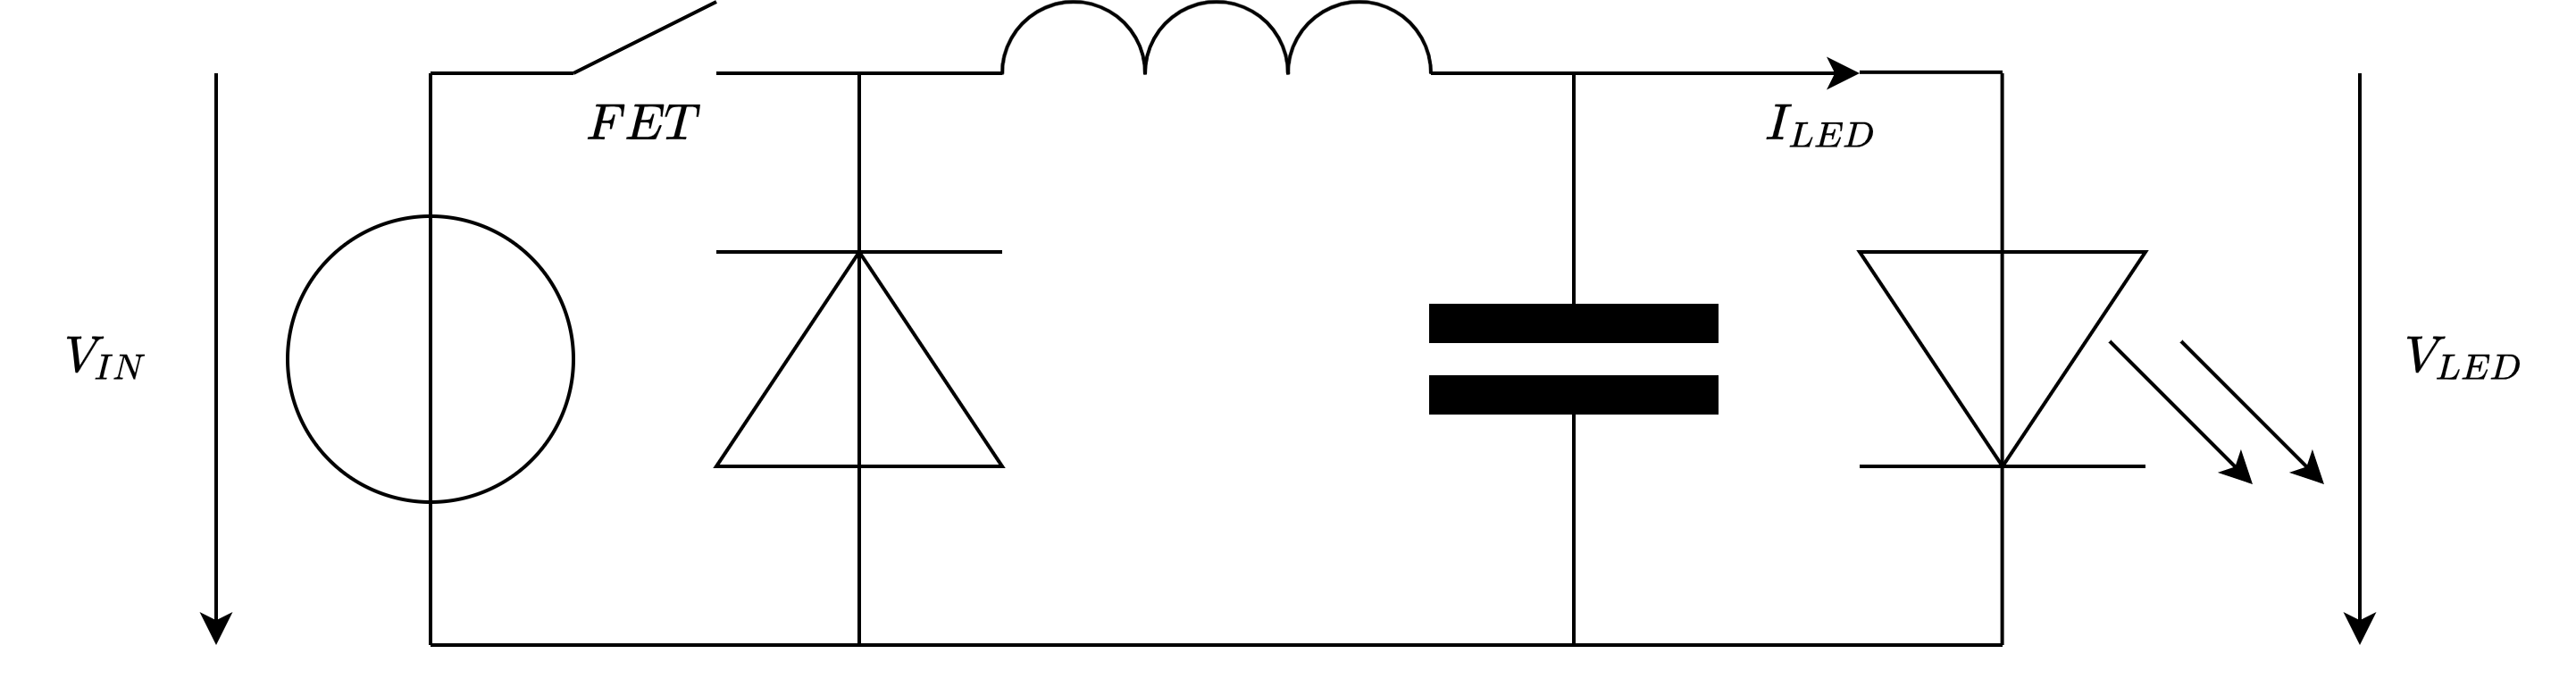
\includegraphics[width=1\linewidth]{images/BAT_Buck-Converter}
		\caption{Buck Converter}
		\label{fig:batbuck-converter}
	\end{figure}
	\subsection{Komponentenwahl}
	Die Wahl der korrekten LED ist bei einem batteriebetriebenen Gerät von enormer Wichtigkeit. Eine ineffiziente LED verringert die Gesamtlaufzeit oder erfordert einen grösseren Akku.
	\subsubsection{Kriterien}
	Für eine effiziente und helle LED sind folgende Kriterien wichtig:
	\begin{itemize}
		\item Lichtleistung 
		\item Wellenlänge
	\end{itemize}
	\subsubsection{Vergleich}
	\begin{table}[H]
		\centering
		\begin{tabular}{|l|p{0.25\textwidth}|l|l|l|}
			\hline
			\textbf{Hersteller} & \textbf{Typ} & \textbf{Farbe} & \textbf{Intensität[mcd]\tablefootnote{bei einem Strom von 2mA}} & \textbf{Spannung[V]} \\ \hline
			SunLED & XZCM2CRK53WA-8VF & Rot & 180 & 2.1 \\ \hline
			SunLED & XZCDGK53W-8VF & Grün & 250 & 3.1 \\ \hline
			SunLED & XZCFBB53W-8VF & Blau & 30 & 3 \\ \hline
			Worldsemi & WS2018 & Rot & 55 & 2.2 \\ \hline
			Worldsemi & WS2018 & Grün & 110 & 3.1 \\ \hline
			Worldsemi & WS2018 & Blau & 20 & 3.4 \\ \hline
			RND & 135-00184 & Rot & 7 & 1.6 \\ \hline
		\end{tabular}
		\caption{Vergleich LED}
		\label{table:vergleich-led}
	\end{table}
	\subsubsection{Fazit}
	Wie im Kapitel \ref{Wellenlänge} ersichtlich, ist die Abwägung zwischen Energieaufnahme der LED und der effektiven Photonenabgabe nicht trivial. Aus technischer Sicht macht dementsprechend eine LED mit einer Wellenlänge von 555nm (Grün) am meisten Sinn. Nach Rücksprache mit dem Industrieparter hEar, dient das Gerät an erster Stelle als Akustik-Warngerät. Warnungen werden üblicherweise mit einer Wellenlänge von 780nm (Rot) gekennzeichnet. Dadurch wird im Endprodukt die Low-Power-LED XZCM2CRK53WA-8V von SunLED eingesetzt.
	\newpage
	\section{Entwicklung}\label{Entwicklung}
	Die im Unterkapitel \ref{Ziele} definierten Ziele sollen nun umgesetzt werden. Dazu soll die von aussen sichtbare Vorderseite möglichst wenig Bauteile aufweisen, um das visuelle Design nicht zu beeinträchtigen. Mit einer angestrebten Gesamtgrösse von 60mm Durchmesser können die gewählten Bauteile geradenoch auf dem PCB in einer symmetrischen Art platziert werden. 
	\subsection{Konzept} \label{Konzept}
	\paragraph{Front}
	Die Vorderseite weist folgende Bauteile auf:
	\begin{itemize}
		\item 8 LEDs
		\item Mikrofon
		\item LED-Treiber-IC
	\end{itemize}
	Zudem sind die LEDs ringförmig angeordnet, um der Anforderung eines visuellen Ladebalkens entsprechen zu können.
	\paragraph{Back}
	Die Rückseite hingegen beinhaltet folgende Bauteile:
	\begin{itemize}
		\item USB-C-Ladeanschluss
		\item Polyfuse (automatisch rückstellbarer Überstromschutz)
		\item Schalter, um generell das Gerät ein- und auszuschalten
		\item BMS, um den Akku sicher auf- und entladen zu können
		\item Mikrocontroller, welcher sich aufgrund seiner Antenne am Rand des PCBs befinden muss
		\item Akkuhalter
		\item Optionaler Speicherbaustein
	\end{itemize}
	\begin{figure}[H]
		\centering
		\includegraphics[width=1\linewidth]{images/BAT_Konzept_Gerät}
		\caption{Konzept PCB-Layout}
		\label{fig:batkonzeptgerat}
	\end{figure}
	\begin{figure}[H]
		\centering
		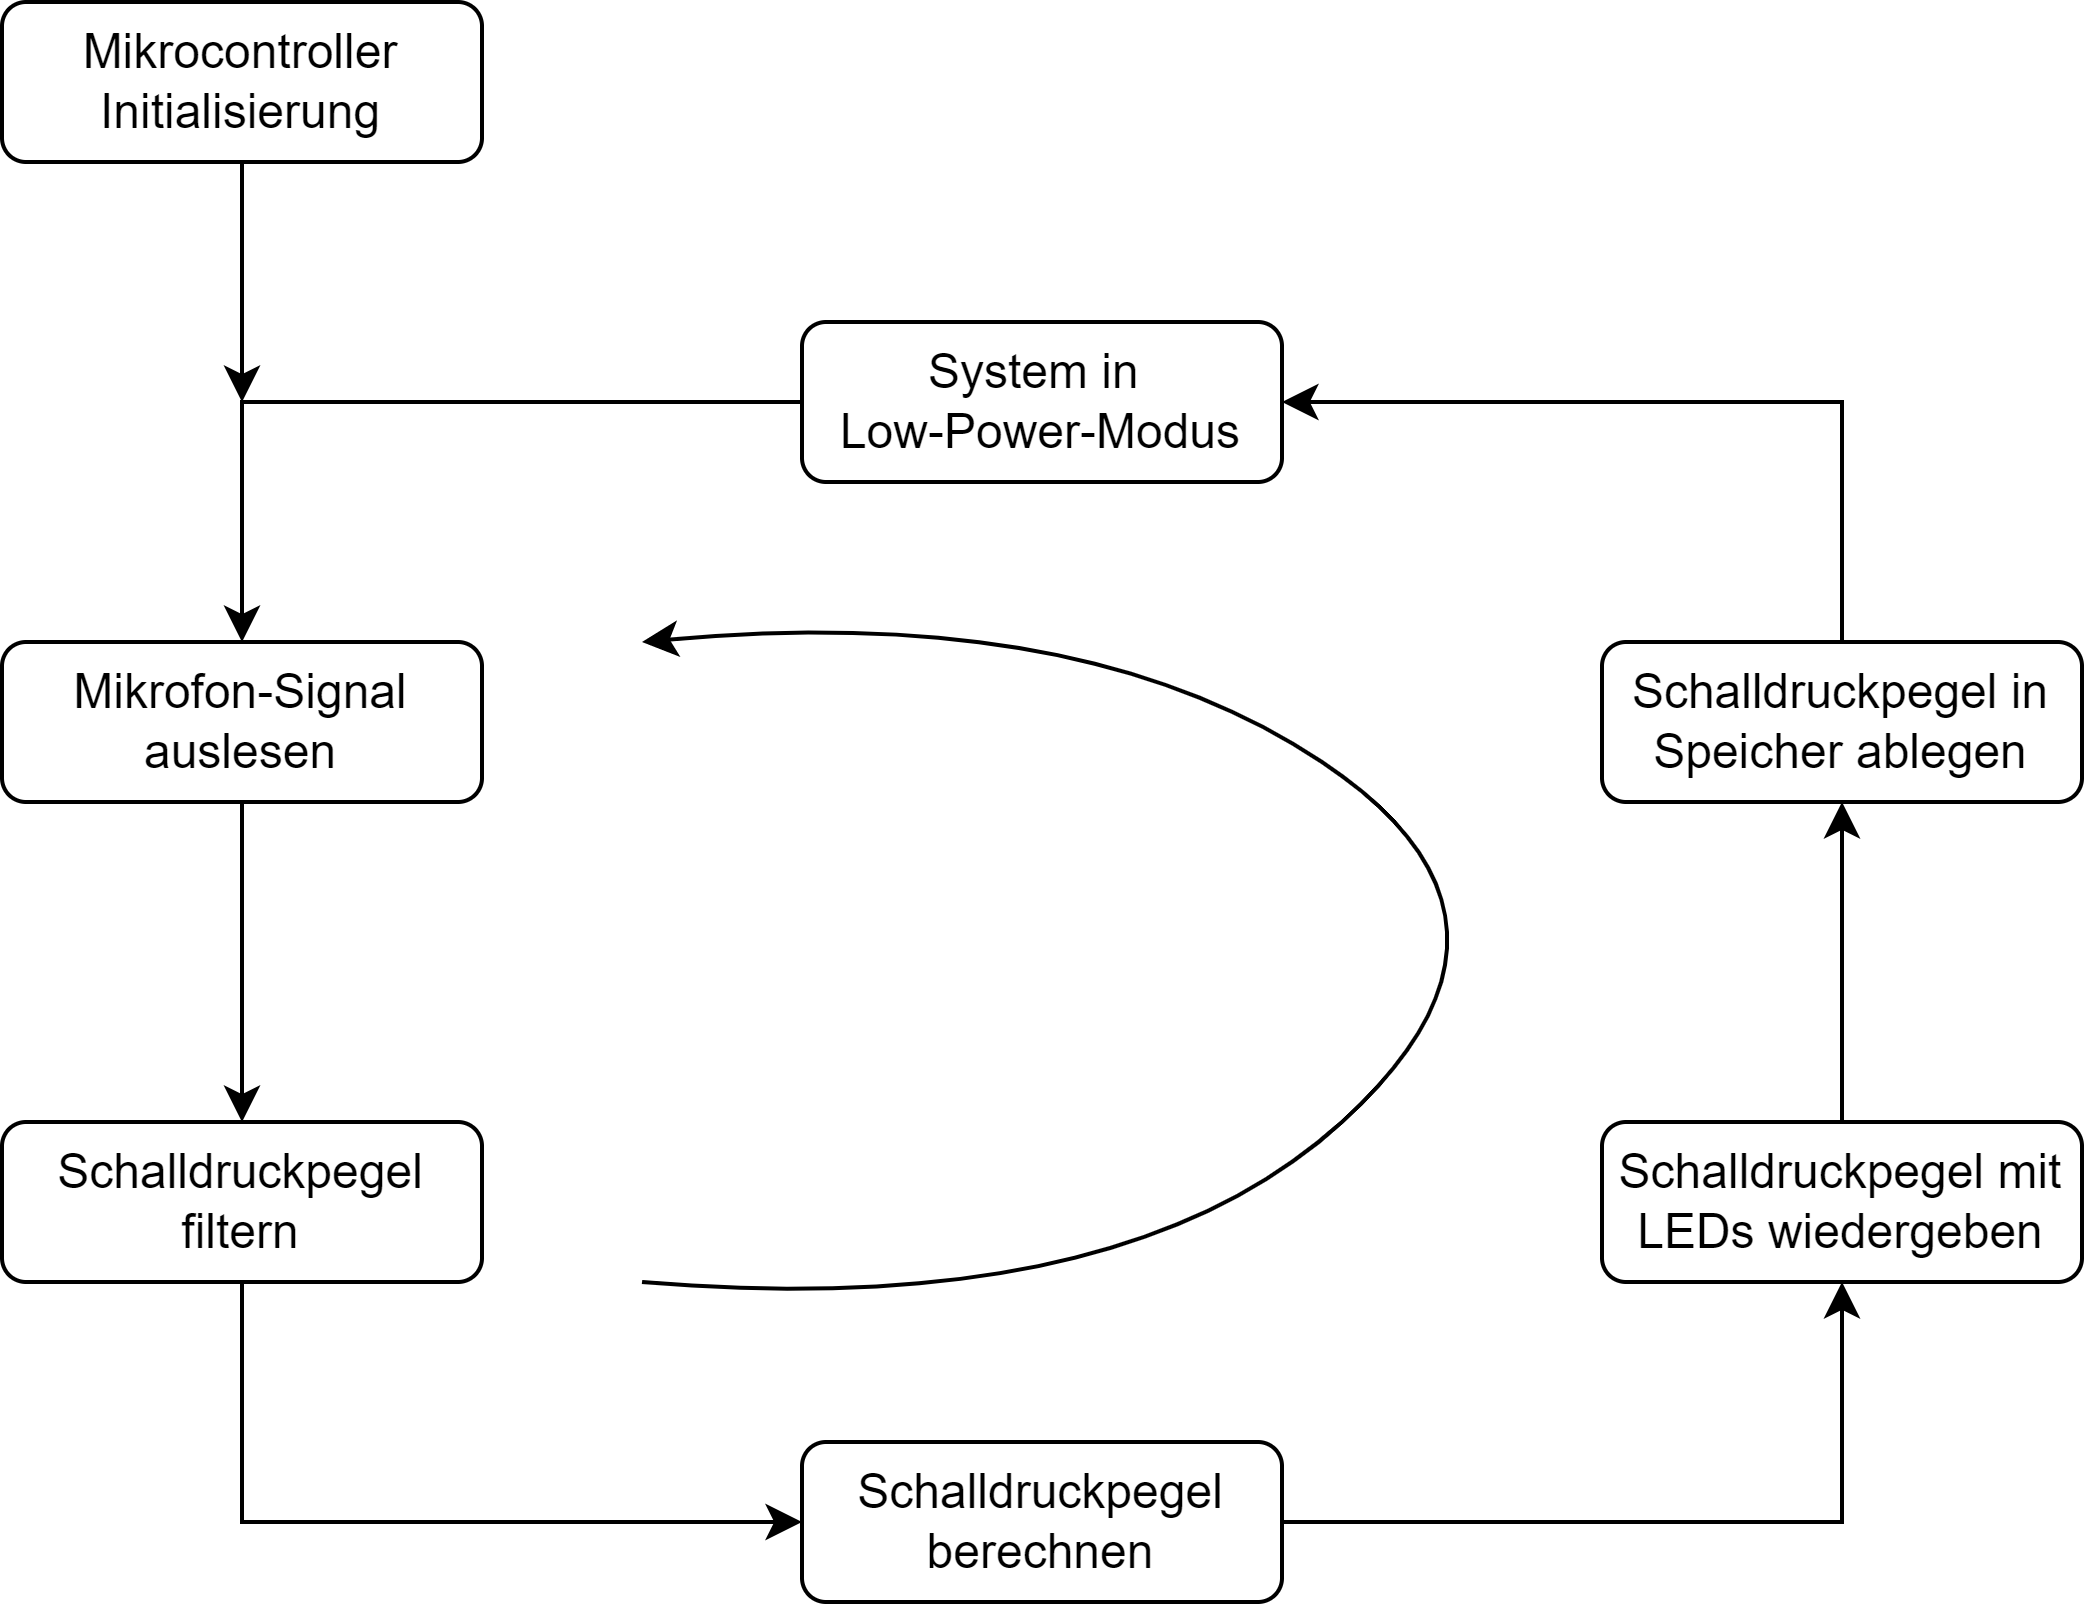
\includegraphics[width=1\linewidth]{images/BAT_Konzept_Softwareablauf}
		\caption{Konzept Softwareablauf}
		\label{fig:batkonzeptsoftwareablauf}
	\end{figure}
	
	\subsection{Hardware}
	Auf Basis des \hyperref[Konzept]{Konzepts} wurde das PCB entworfen. Dabei wurde für die optimale Platzierung, sowie die zusätzlichen Widerstände und Kondensatoren, die jeweiligen Datenblätter der Hersteller konsultiert.
	\subsubsection{PCB}
	Das PCB durchlief dabei mehrere Iterationen. Nachfolgend treten die Ände\-rungen mit den benötigten Zusatzinformationen chronologisch auf \footnote{Detailierte Abbildungen der Versionen befinden sich im Anhang \ref{PCB-Versionen}}. Zudem befindet sich nachfolgend eine Übersicht, wieso, welches Bauteil eingesetzt wird.
	\paragraph{V1-1}\mbox{}\\
	Lediglich kleinere Verdrahtungs- und Platzierungsoptimierungen
	\paragraph{V1-2}\mbox{}\\
	Folgende Anpassungen wurden vorgenommen:
	\begin{itemize}
		\item Akku-Verpolungsschutz mittels \nameref{P-Kanal MOSFET}
		\item Testpads für I²C, SPI und PDM entfernt
		\item USB-C 16 Pin Buchse durch 6 Pin Buchse (power only) ersetzt
		\item Rotation der LEDs um 40° im Gegenuhrzeigersinn, um die Reihenfolge der LEDs zu gewährleisten. Zusätzliche Optimierung der Platzierung der LEDs, um die Verdrahtung zu vereinfachen.
		\item TRIG-Pin des LED-Treiber-ICs auf Masse geschaltet
		\item Spannungsteiler zur Messung der Speisespannung via USB-C
		\item Optionaler Pullup-Widerstand an DRV\_EN, um den Anschluss nicht immer manuell schalten zu müssen
	\end{itemize}
	\paragraph{V1-3}\mbox{}\\
	Auf Wunsch von hEar wurde zusätzlich noch ein PCB entwickelt, welches funktionsidentisch mit dem Vorgänger ist. Einzig die LEDs sind nun nicht mehr ringförmig angeordnet, sondern erstrecken sich neu auf einer vertikalen Linie.
	\paragraph{Sicherung}\mbox{}\\
	Im falle eines Kurzschlusses auf Geräteseite wird mittels einer rückstellbaren Sicherung (PPTC\footnote{\textbf{P}olymeric \textbf{P}ositive \textbf{T}emperature \textbf{C}oefficient, automatisch rückstellbare Sicherung von Littlefuse}) der Stromfluss unterbrochen. Die gewählte Sicherung blockiert bei einem Strom von 400mA komplett und setzt sich automatisch wieder zurück, sobald die Speisung abgetrennt wird.
	\paragraph{LED-Treiber} \mbox{}\\
	Die Aufgabe des Treibers ist es, den LED-Strom möglichst Energieeffizient zu regeln (siehe \ref{Vorwiderstand}). Der gewählte Treiber ermöglicht es, alle 8 LEDs individuell in 100uA-Schritten zu regeln. So kann die Energieaufnahme des Gesamtsystems kontrolliert werden.
	\paragraph{Akku-Laderegler $\vert$ BMS} \mbox{}\\
	Das \textbf{B}attery \textbf{M}anagement \textbf{S}ystem wurde aufgrund folgender, benötigter Eigenschaften gewählt:
	\begin{itemize}
		\item Möglichst wenige externe Bauteile
		\item Über- und Unterspannungsschutz
		\item Überstromschutz
		\item Keine direkte Ansteuerung mittels Mikrocontroller nötig
		\item Möglichkeit zur visuellen Darstellung des Ladestatus
		\item Unterstützung von Li-Po und Li-Ion Akkus
	\end{itemize}
	\paragraph{Spannungsregler} \mbox{}\\
	Der Akku weist eine maximale Nennspannung von 4.2V (Typ. 3.6V) auf. Alle gewählten Halbleiter erlauben jedoch maximal eine Speisespannung von 3.6V. Dadurch wird ein möglichst effizienter und kostengünstiger Spannungs\-regler verwendet. Wie auch bereits das BMS, weist der Spannungsregler möglichst wenig externe Bauteile auf.
	\paragraph{USB-C-Buchse}\mbox{}\\
	Die in V1-0 verwendete Buchse (16 Pin) wird durch eine 6 Pin (power only) ersetzt. Dies, da die ursprünglich geplante Möglichkeit, den Mikrocontroller via USB zu programmieren, wieder verworfen wurde. Dies, weil auf den geplanten Anschlüssen zeitweise 5 V vom USB-Standard anliegen. Dadurch kann eine kostenoptimiertere Buchse verwendet werden.
	\paragraph{P-Kanal MOSFET} \label{P-Kanal MOSFET} \mbox{}\\
	Für den Verpolungsschutz kann im Grunde auch eine simple Diode (oder Schottky-Diode\footnote{Die Schwellspannung entspricht nur ca. 0.2V}) verwendet werden. Der daraus folgende Spannungsabfall ist jedoch für ein akkubetriebenes Gerät nicht ideal. Die Lösung bietet ein P-Kanal-MOSFET, wie in Abbildung \ref{fig:batverpolungsschutz} ersichtlich. Die Z-Diode, sowie der Gate-Widerstand, werden jedoch weggelassen, da die Batteriespannung die maximale Source-Gate-Spannung des gewählten FETs nicht überschreitet.
	\begin{figure}[H]
		\centering
		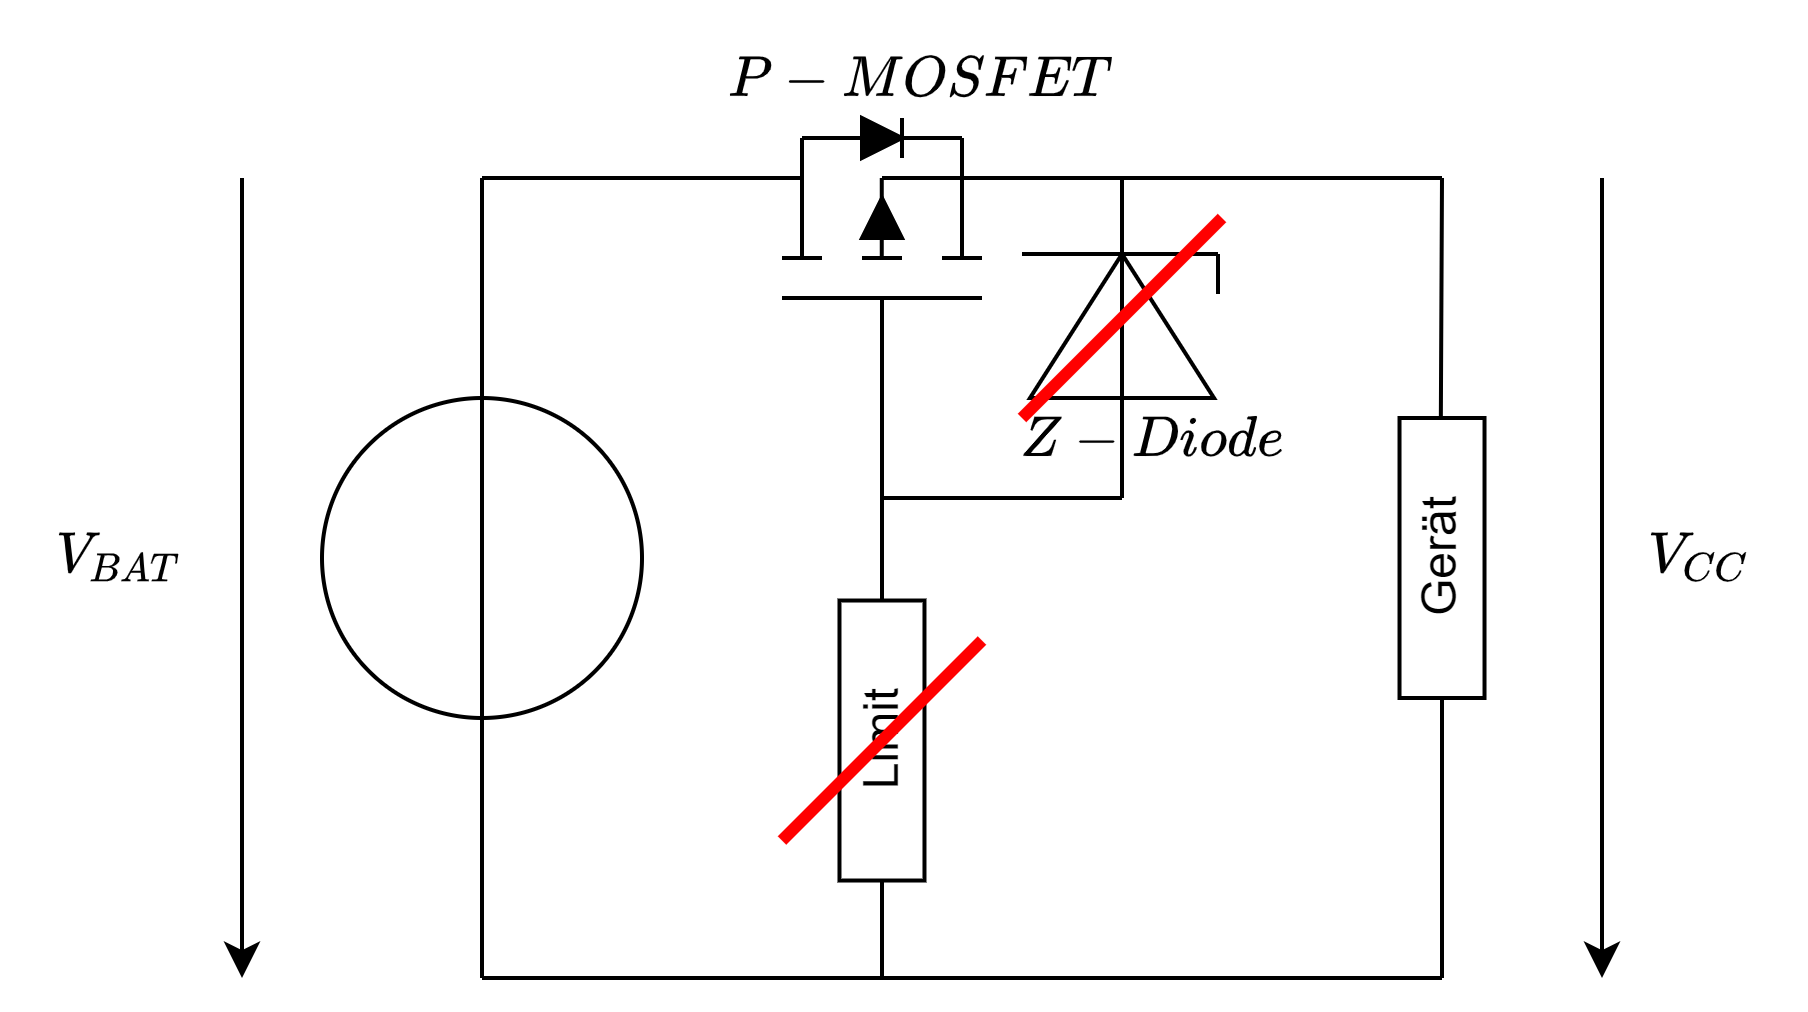
\includegraphics[width=0.7\linewidth]{images/BAT_Verpolungsschutz}
		\caption{Verpolungsschutz mittels P-Kanal MOSFET}
		\label{fig:batverpolungsschutz}
	\end{figure}
	
	\subsubsection{Kosten} \label{Kosten}
	Die Tabelle \ref{table:materialliste} beinhaltet alle anfallenden Materialkosten exkl. Versand. Zudem wurde \href{https://jlcpcb.com/}{JLCPCB} als PCB-Hersteller gewählt, da zum einen die Qualität bei 2-Layer-PCBs ausreicht und zum anderen mit der Anbindung an \href{https://www.lcsc.com/}{LCSC} die Bestückung der PCBs direkt im selben Werk stattfindet. Dadurch verkürzt sich die Fertigung des Endproduktes. \\
	Die vorhandenen Kondensatoren, sowie die benötigten Widerstände werden in der Tabelle \ref{table:materialliste} unter Diverse zusammengenommen. Dies aus dem Grund, da keines dieser Bauteile einer besonderen Toleranz unterliegt. Dadurch kann bei der PCB-Bestellung eine kostenoptimierte Wahl getroffen werden.
\begin{table}[!ht]
	\centering
	\begin{tabular}{|l|l|l|l|}
		\hline
		\textbf{Hersteller} & \textbf{Typ} & \textbf{Bezeichnung} & \textbf{Preis/100} \\ \hline
		JLCPCB & \href{https://cart.jlcpcb.com/quote?orderType=1\&stencilLayer=2\&stencilWidth=40\&stencilLength=40\&stencilCounts=100}{-} & PCB inkl. Versand & 0.394 \\ \hline
		Texas Instruments  & \href{https://www.mouser.ch/ProductDetail/Texas-Instruments/BQ21040DBVR?qs=cttFivMKqWyovUuY6Xwwcw\%3D\%3D}{BQ21040DBVR} & Batterie-Management & 0.516 \\ \hline
		Microchip Technology & \href{https://www.mouser.ch/ProductDetail/Microchip-Technology/MIC5504-3.3YM5-TR?qs=U6T8BxXiZAUmVQ5Zs217qQ\%3D\%3D}{MIC5504-3.3YM5-TR}  & 3V3 LDO & 0.095 \\ \hline
		RS PRO & \href{https://ch.rs-online.com/web/p/knopfzellen-akkus/1834296}{LIR2477} & Akku & 4.085 \\ \hline
		Littlefuse & \href{https://www.mouser.ch/ProductDetail/Littelfuse/1210L020WR?qs=PWhpLWeW8wcFhN6lPv0ohQ%3D%3D}{1210L020WR} & Rückstellbare Sicherung & 0.205 \\ \hline
		Texas Instruments  & \href{https://www.mouser.ch/ProductDetail/Texas-Instruments/LP55231SQX-NOPB?qs=HF2YfZwisE8IcIRPR19gTw\%3D\%3D}{LP55231SQX/NOPB}  & 9-Kanal LED-Treiber & 1.35 \\ \hline
		SunLED & \href{https://www.digikey.ch/de/products/detail/sunled/XZCM2CRK53WA-8VF/10449794}{XZCM2CRK53WA-8VF} & LED RED CLEAR & 0.2072 \\ \hline
		C\&K & \href{https://www.mouser.ch/ProductDetail/CK/JS102011SAQN?qs=LgMIjt8LuD\%252B69bNM9a\%2FozQ\%3D\%3D}{JS102011SAQN}  & Schalter 0.3A@6V & 0.453 \\ \hline
		Keystone Electronics & \href{https://www.mouser.ch/ProductDetail/Keystone-Electronics/1025-7?qs=2eeJ4RqLicExTS\%2FpSQucQQ\%3D\%3D}{1025-7}  & Batteriehalter & 1.26 \\ \hline
		STMicroelectronics & \href{https://www.mouser.ch/ProductDetail/STMicroelectronics/M95P16-IXMNT-E?qs=rQFj71Wb1eV9LflyHvgrDg\%3D\%3D}{M95P16-IXMNT/E}  & 16MBit SPI EEPROM & 0.843 \\ \hline
		Silicon Labs & \href{https://www.mouser.ch/ProductDetail/Silicon-Labs/BGM220PC22WGA2R?qs=7MVldsJ5UayRQss0gz56jA\%3D\%3D}{BGM220PC22WGA2R}  & Mikrocontroller & 6.33 \\ \hline
		TDK InvenSense & \href{https://www.mouser.ch/ProductDetail/TDK-InvenSense/ICS-41351?qs=\%252B6g0mu59x7LDJ1mBnROZzA\%3D\%3D}{ICS-41351}  & MEMS-Mikrofon & 1.05 \\ \hline
		GCT & \href{https://www.mouser.ch/ProductDetail/GCT/USB4125-GF-A?qs=KUoIvG\%2F9IlaIQ4zBJ6gLeA\%3D\%3D}{640-USB4125-GF-A} & USB-C Buchse 6 Pin & 0.381 \\ \hline
		Toshiba & \href{https://www.mouser.ch/ProductDetail/Toshiba/SSM3J334RLF?qs=PiFplXvYe5VBSYhr6TJz8A\%3D\%3D}{SSM3J334R,LF} & P-Channel MOSFET & 0.109 \\ \hline
		Diverse & Capacitor \& Resistor & Abmessung: 0603 [Inch] & 0.6 \\\hline
		~ & ~ & ~ & \textbf{17.90 CHF} \\ \hline
	\end{tabular}
	\caption{Materialliste $\vert$ Stand: 01.04.2024}
	\label{table:materialliste}
\end{table}
	\subsection{Software}
	Im Kern besteht die Software, wie in Abbildung \ref{fig:batkonzeptsoftwareablauf} gezeigt, aus einem einzelnen, sich wiederholenden Kreis. Durch den einfach gehaltenen Ablauf wird auf den Einsatz eines RTOS verzichtet. Um diesen Abschnitt übersichtlich zu halten sind Timing-Diagramme sowie die Software im Anhang \ref{Anhang:Software} zu finden.
	\subsubsection*{Timer} \label{Timer}
	Die Timer-Implementation dient als Hauptschleife, um die Datenaggregation, Verarbeitung und Ausgabe steuern zu können. \\Das Makro \textbf{BAT\_MEASUREMENT\_INTERVAL} ermöglicht es, auf wenige Millisekunden genau die Schlaufe zu steuern. Die Programmabfolge ist in Abbildung \ref{fig:batsoftwareletimer} ersichtlich.
	\begin{figure}[H]
		\centering
		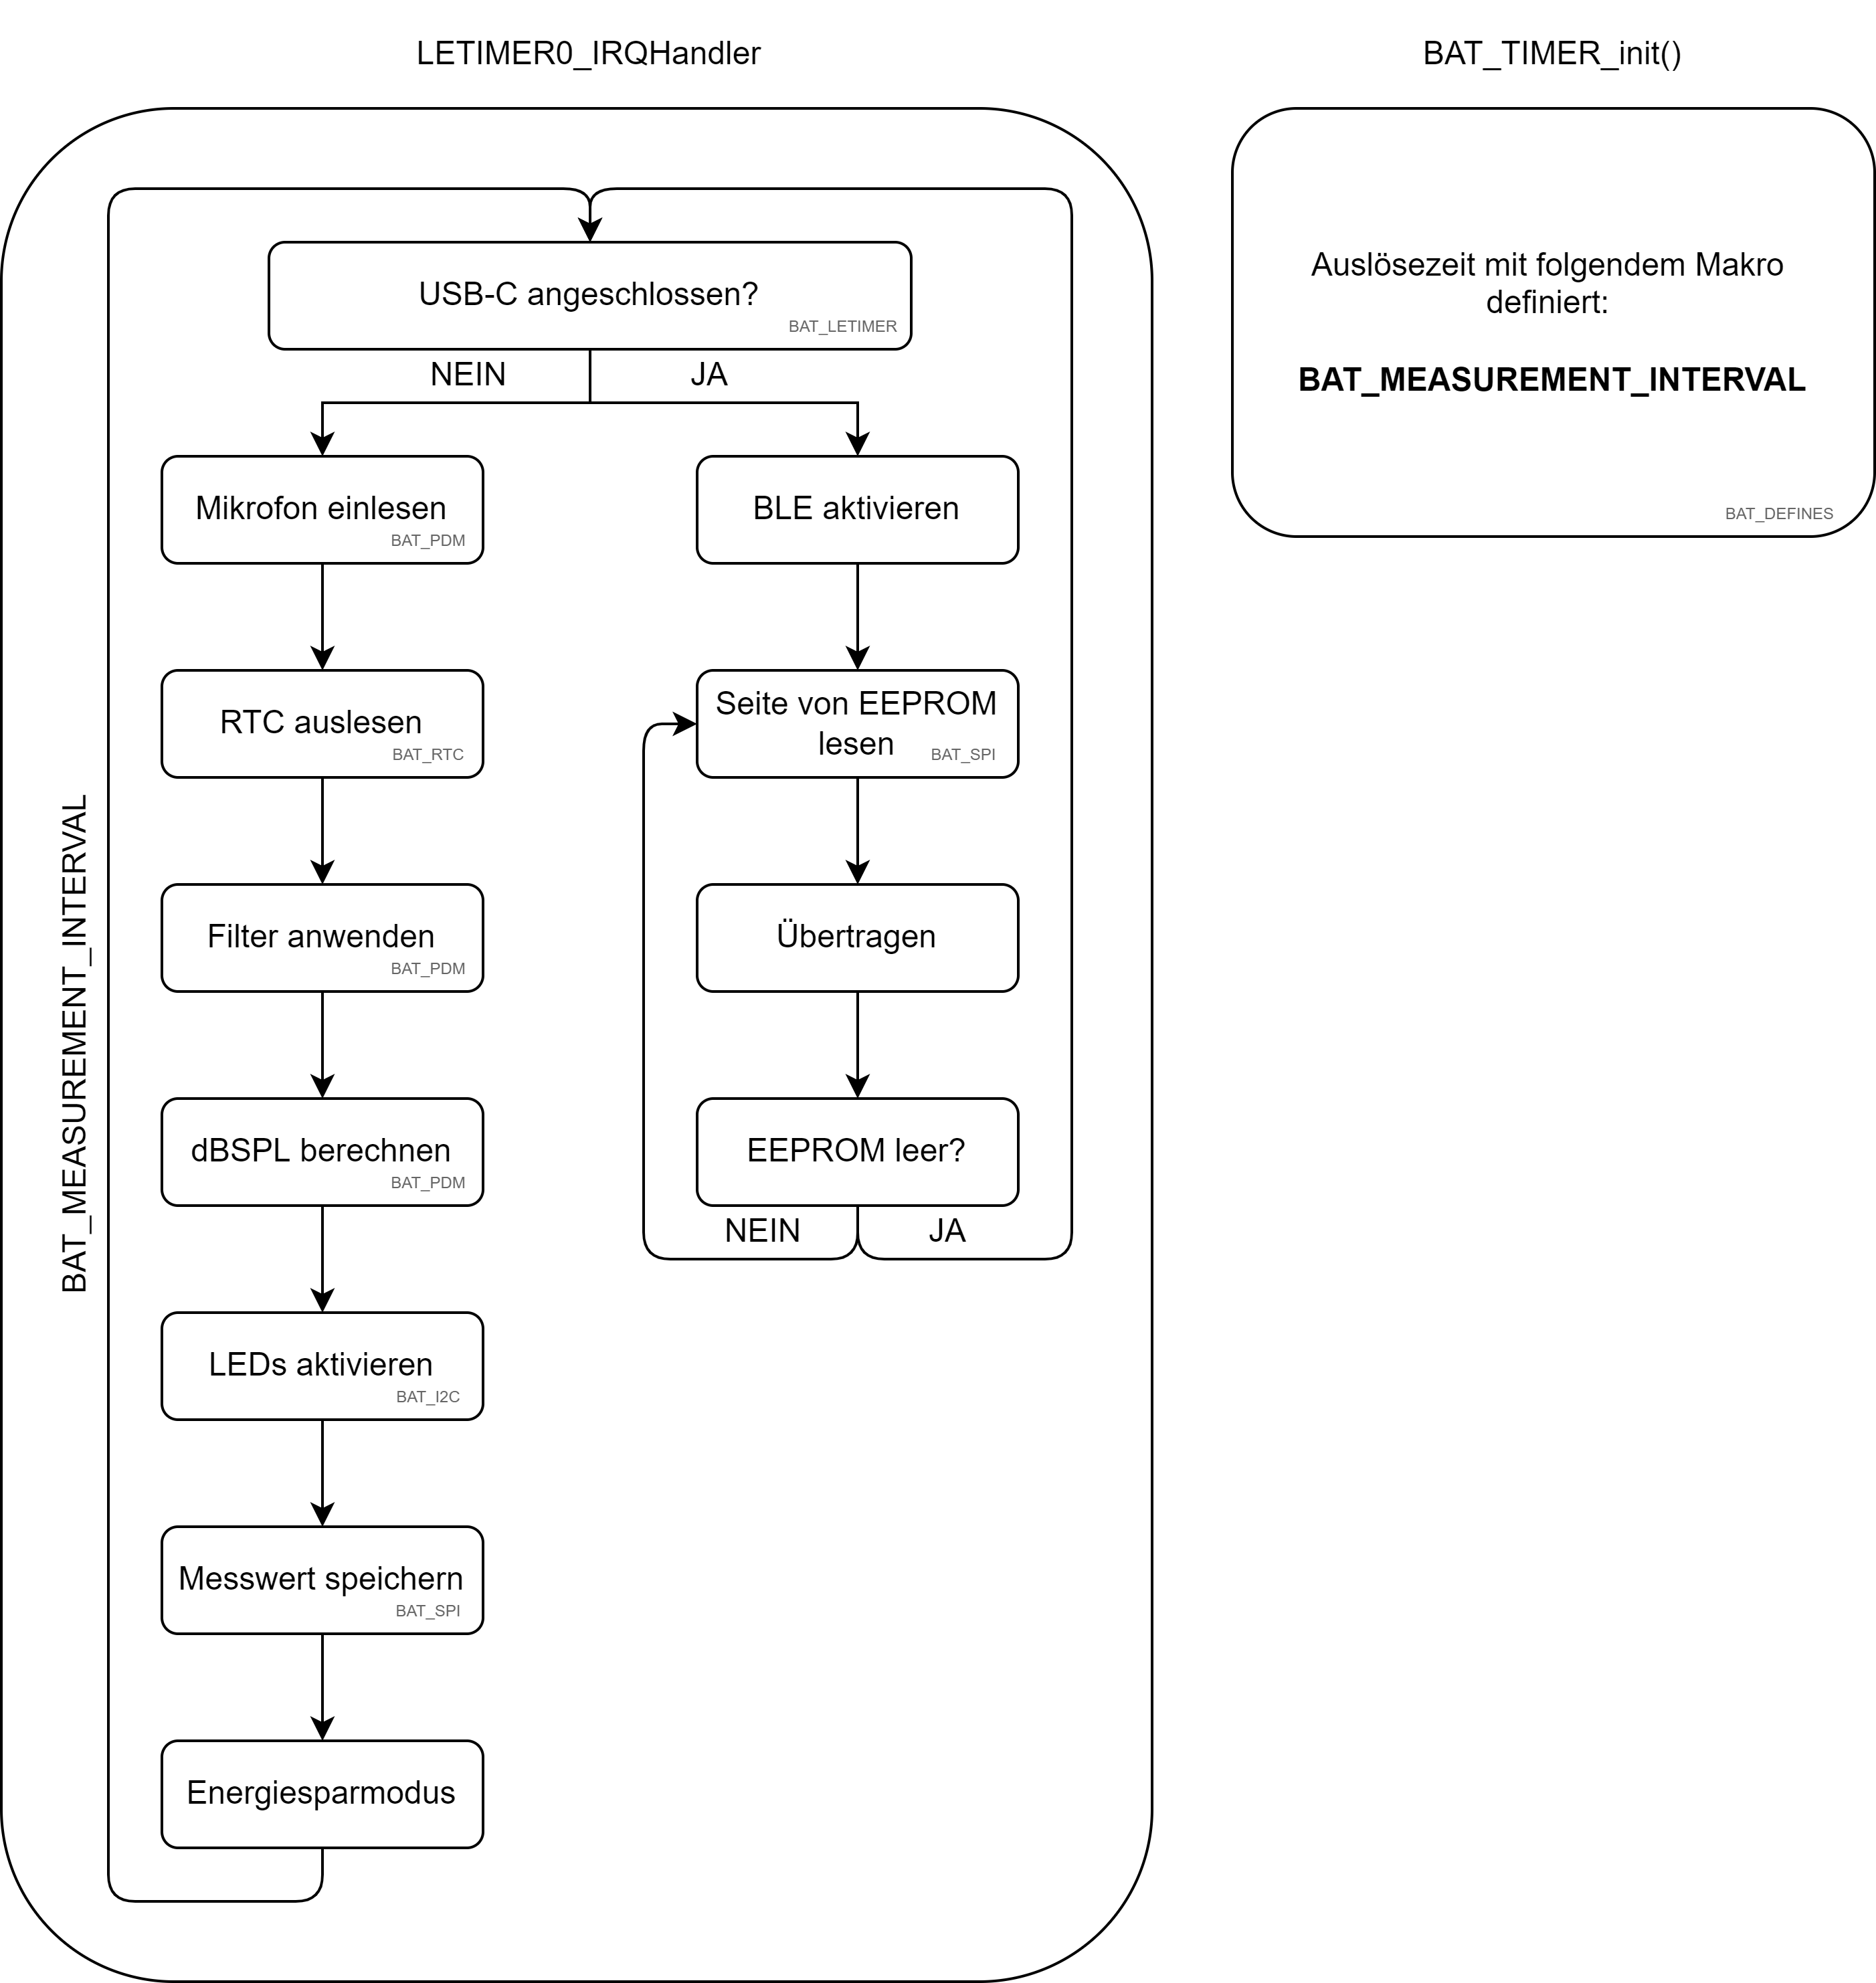
\includegraphics[width=1\linewidth]{images/BAT_Software_LETIMER}
		\caption{Übersicht zu (LE)Timer-Funktionalität}
		\label{fig:batsoftwareletimer}
	\end{figure}
	\subsubsection*{Filterdesign}
	Wie im Unterkapitel \ref{Frequenzbewertung} erläutert, reagiert unser Gehör nicht auf alle Frequenzen gleich. Um diese Frequenzbewertung in die Schalldruckpegel-Be\-rechnung einfliessen zu lassen, wird ein digitales, diskretes Filter benötigt. Die verwendeten Frequenzbewertungsfilter sind jedoch ausschliesslich in der S-Ebene (Laplace-Bereich, zeitkontinuierlich) erhältlich. Diesbezüglich stehen, wie in Abbildung \ref{fig:batfrequenzgewichtung} ersichtlich, zwei Wege offen:
	\begin{itemize}
		\item \textbf{Frequenzbereich} \\
		Hier wird das PCM-codierte Signal mittels einer Fast Fourier Transformation (FFT) in den Frequenzbereich transformiert. Anschliessend können die Formeln \ref{G_A_s} oder \ref{G_C_s} auf das Signal angewendet werden, um die gewünschte Gewichtung vorzunehmen. Um anschliessend den Schalldruckpegel berechnen zu können, muss das Signal mittels einer inversen FFT wieder in den Zeitbereich transformiert werden. Je genauer die Frequenzbewertung sein soll, desto kleiner sind die Abstufungen von FFT und IFFT zu wählen, was zu einer Erhöhung des Berechnungsaufwandes auf dem Mikrocontroller führt.
		\item \textbf{Zeitbereich} \\
		Im Gegensatz zum Frequenzbereich muss das PCM-codierte Signal nicht erst in den Frequenzbereich transformiert werden, sondern es kann direkt durch das zeitdiskrete Filter die Gewichtung vorgenommen werden. Dabei treten jedoch zwei Hauptprobleme auf: 
		\begin{itemize}
			\item Ein diskretes Filter im Zeitbereich ist immer nur eine Approximation eines Filters im Frequenzbereich. Dies verringert die Genauig\-keit des implementierten Filters. 
			\item Die Umwandlung eines zeitkontinuierlichen Filters in einen zeitdiskreten ist nicht trivial. Dadurch muss dieser mit beispielsweise der bilinaren Transformation \cite{oppenheim_alan_v_zeitdiskrete_1989} vom Frequenz- in den Zeitbereich transformiert werden. 
		\end{itemize} Die benötigten A- und C-Gewichtungsfilter sind bereits in Matlab \footnote{filterBuilder, Signal Processing Toolbox} inkludiert. Somit können die Filterkoeffizienten direkt exportiert und in C-Code implementiert werden.
	\end{itemize}
	\begin{equation}\label{G_A_s}
		G_A(s) = \frac{7.39705 \cdot 10^9 \cdot s^4}{(s+129.4)^2\cdot (s+676.7)\cdot (s+4636)\cdot (s+76617)^2}
	\end{equation}
		\begin{equation}\label{G_C_s}
		G_C	(s) = \frac{5,91797 \cdot 10^9 \cdot s^2}{(s+129,4)^2\cdot (s+76617)^2}
	\end{equation}
	\begin{figure}[H]
		\centering
		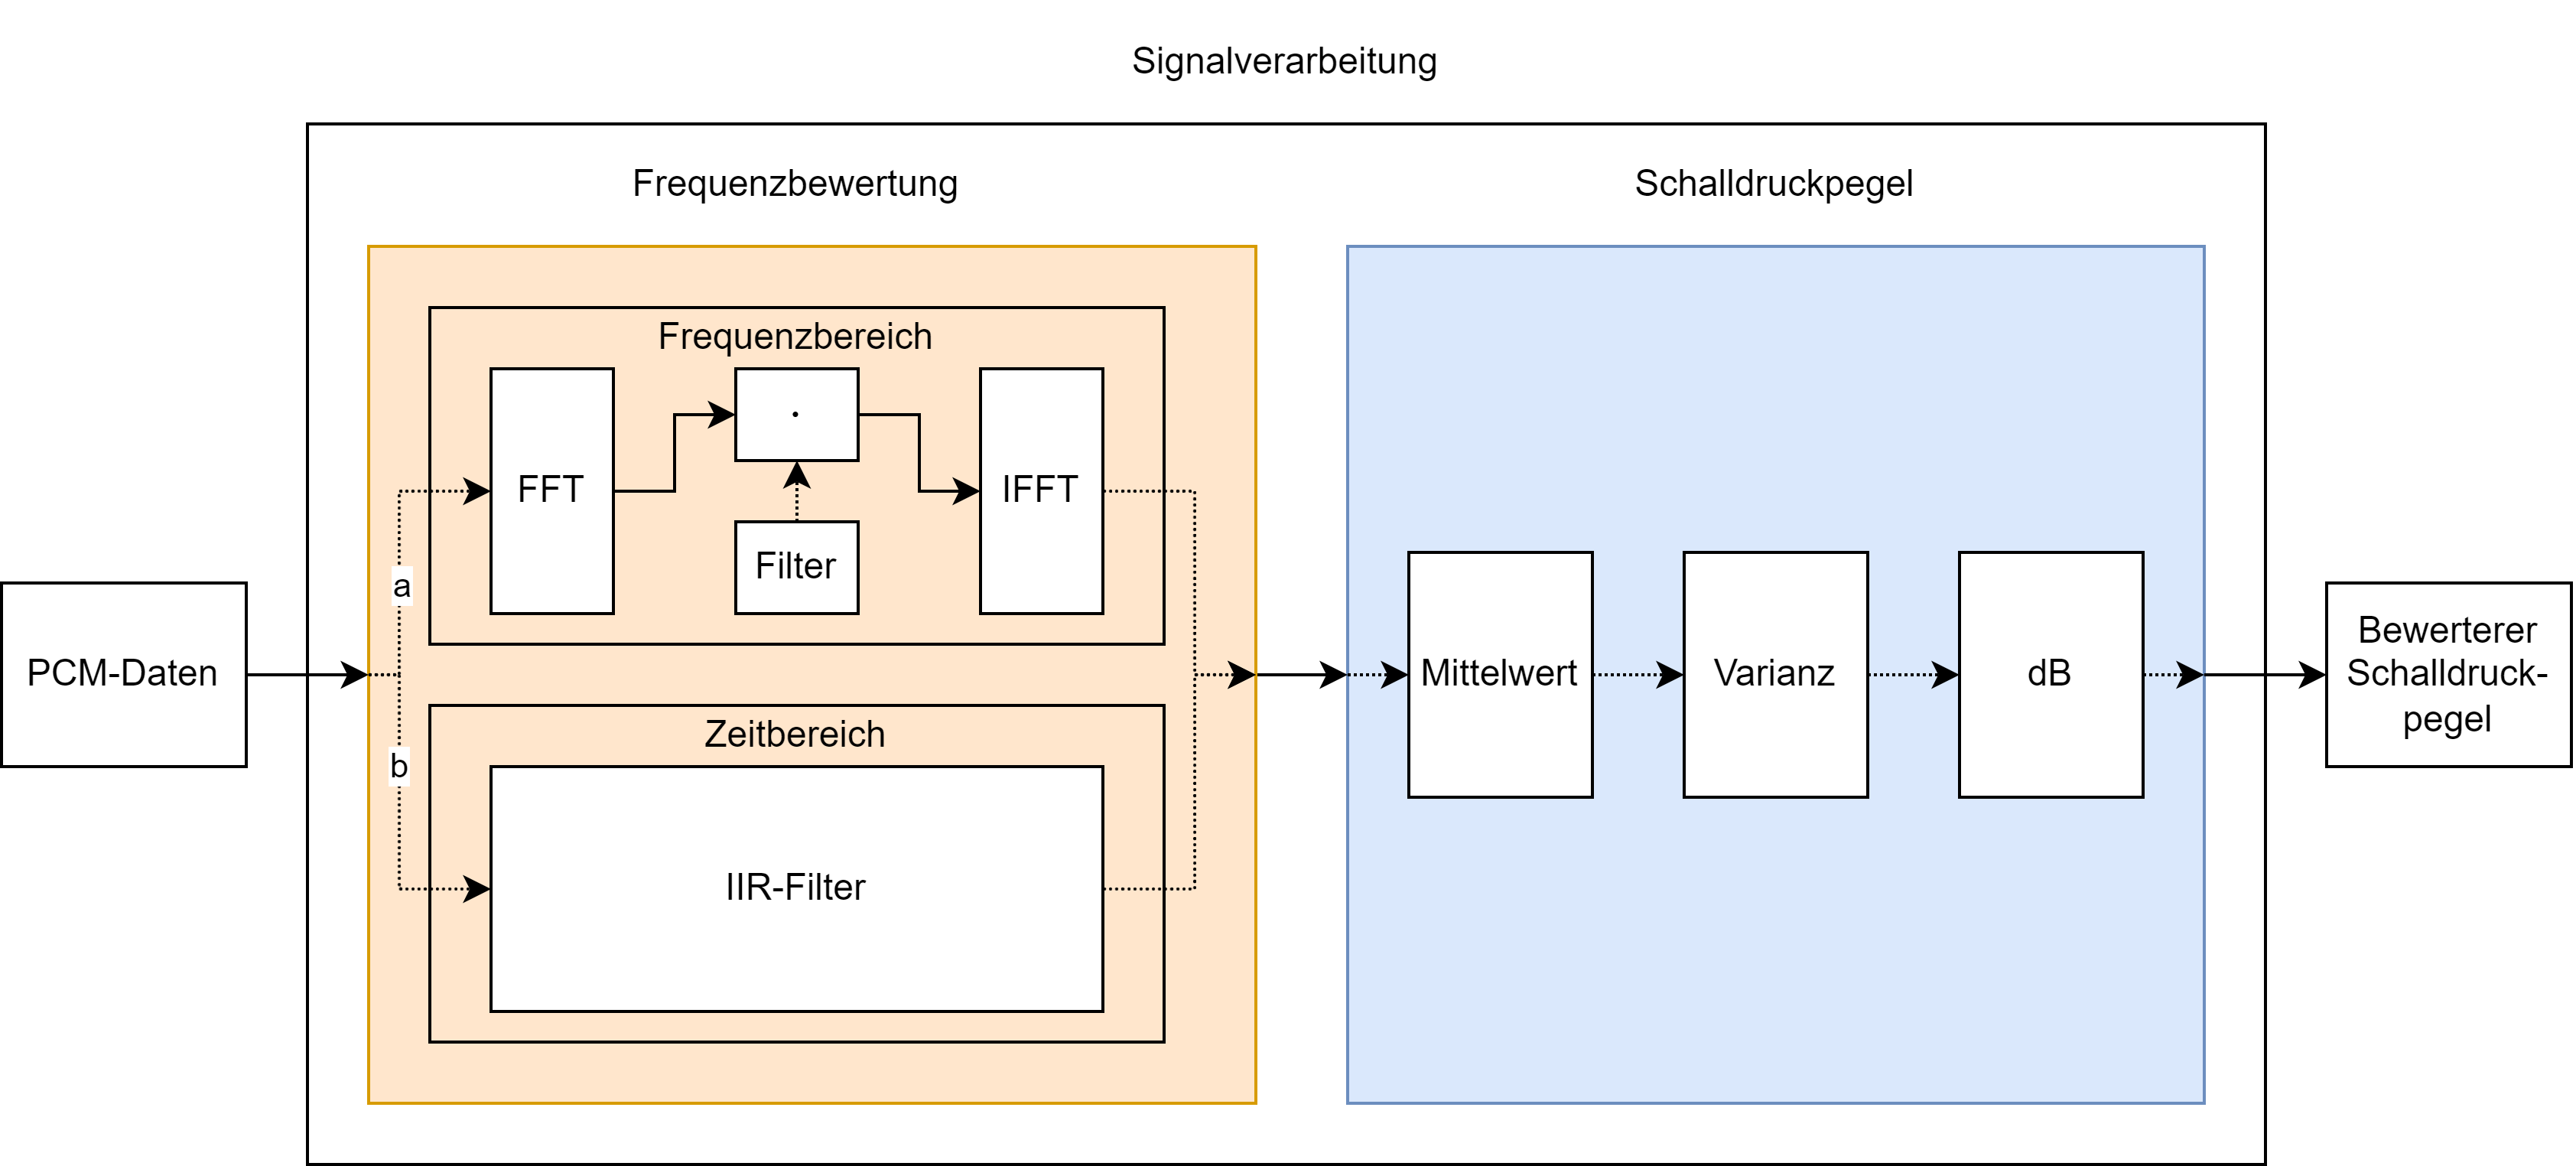
\includegraphics[width=1\linewidth]{images/BAT_Frequenzgewichtung}
		\caption{Unterschied Zeit- und Frequenzbereich zur Frequenzgewichtung}
		\label{fig:batfrequenzgewichtung}
	\end{figure}
	\subsubsection*{Filterimplementation}
	Die aus Matlab exportieren Filterkoeffizienten weisen einen entscheidenden Unterschied zu gewöhnlichen IIR-Filterkoeffizienten auf. Der Gesamtfilter wird in Teilfilter, sogenannte BiQuads, aufgeteilt, welche anschliessend kaskad\-iert werden. Dies, weil die Stabilität von Filtern mit tiefer Ordnung leichter kontrolliert werden kann als bei jenen mit einer hohen Ordnung. Dadurch besteht ein einzelnes BiQuad-Filter-Element jeweils aus einem IIR-Filter zweiter Ordnung. Dabei existieren, wie in Abbildung \ref{fig:batbiquad-uebersicht} aufgezeigt, vier verschiedene Arten der BiQuad-Implementation. Oftmals verfügen Mikrocontroller bereits über eine Hardware-Implementation einer dieser Arten. Der in dieser Arbeit gewählte jedoch nicht. Die Wahl der Implementation ist dadurch frei. Aus diesem Grund wurde die "Transposed Direct Form 2" gewählt. Dies, da diese zwar mehr Variablen zur als Zwischenspeicher, jedoch weniger Rechenoperationen benötigt.
	\begin{figure}[H]
		\centering
		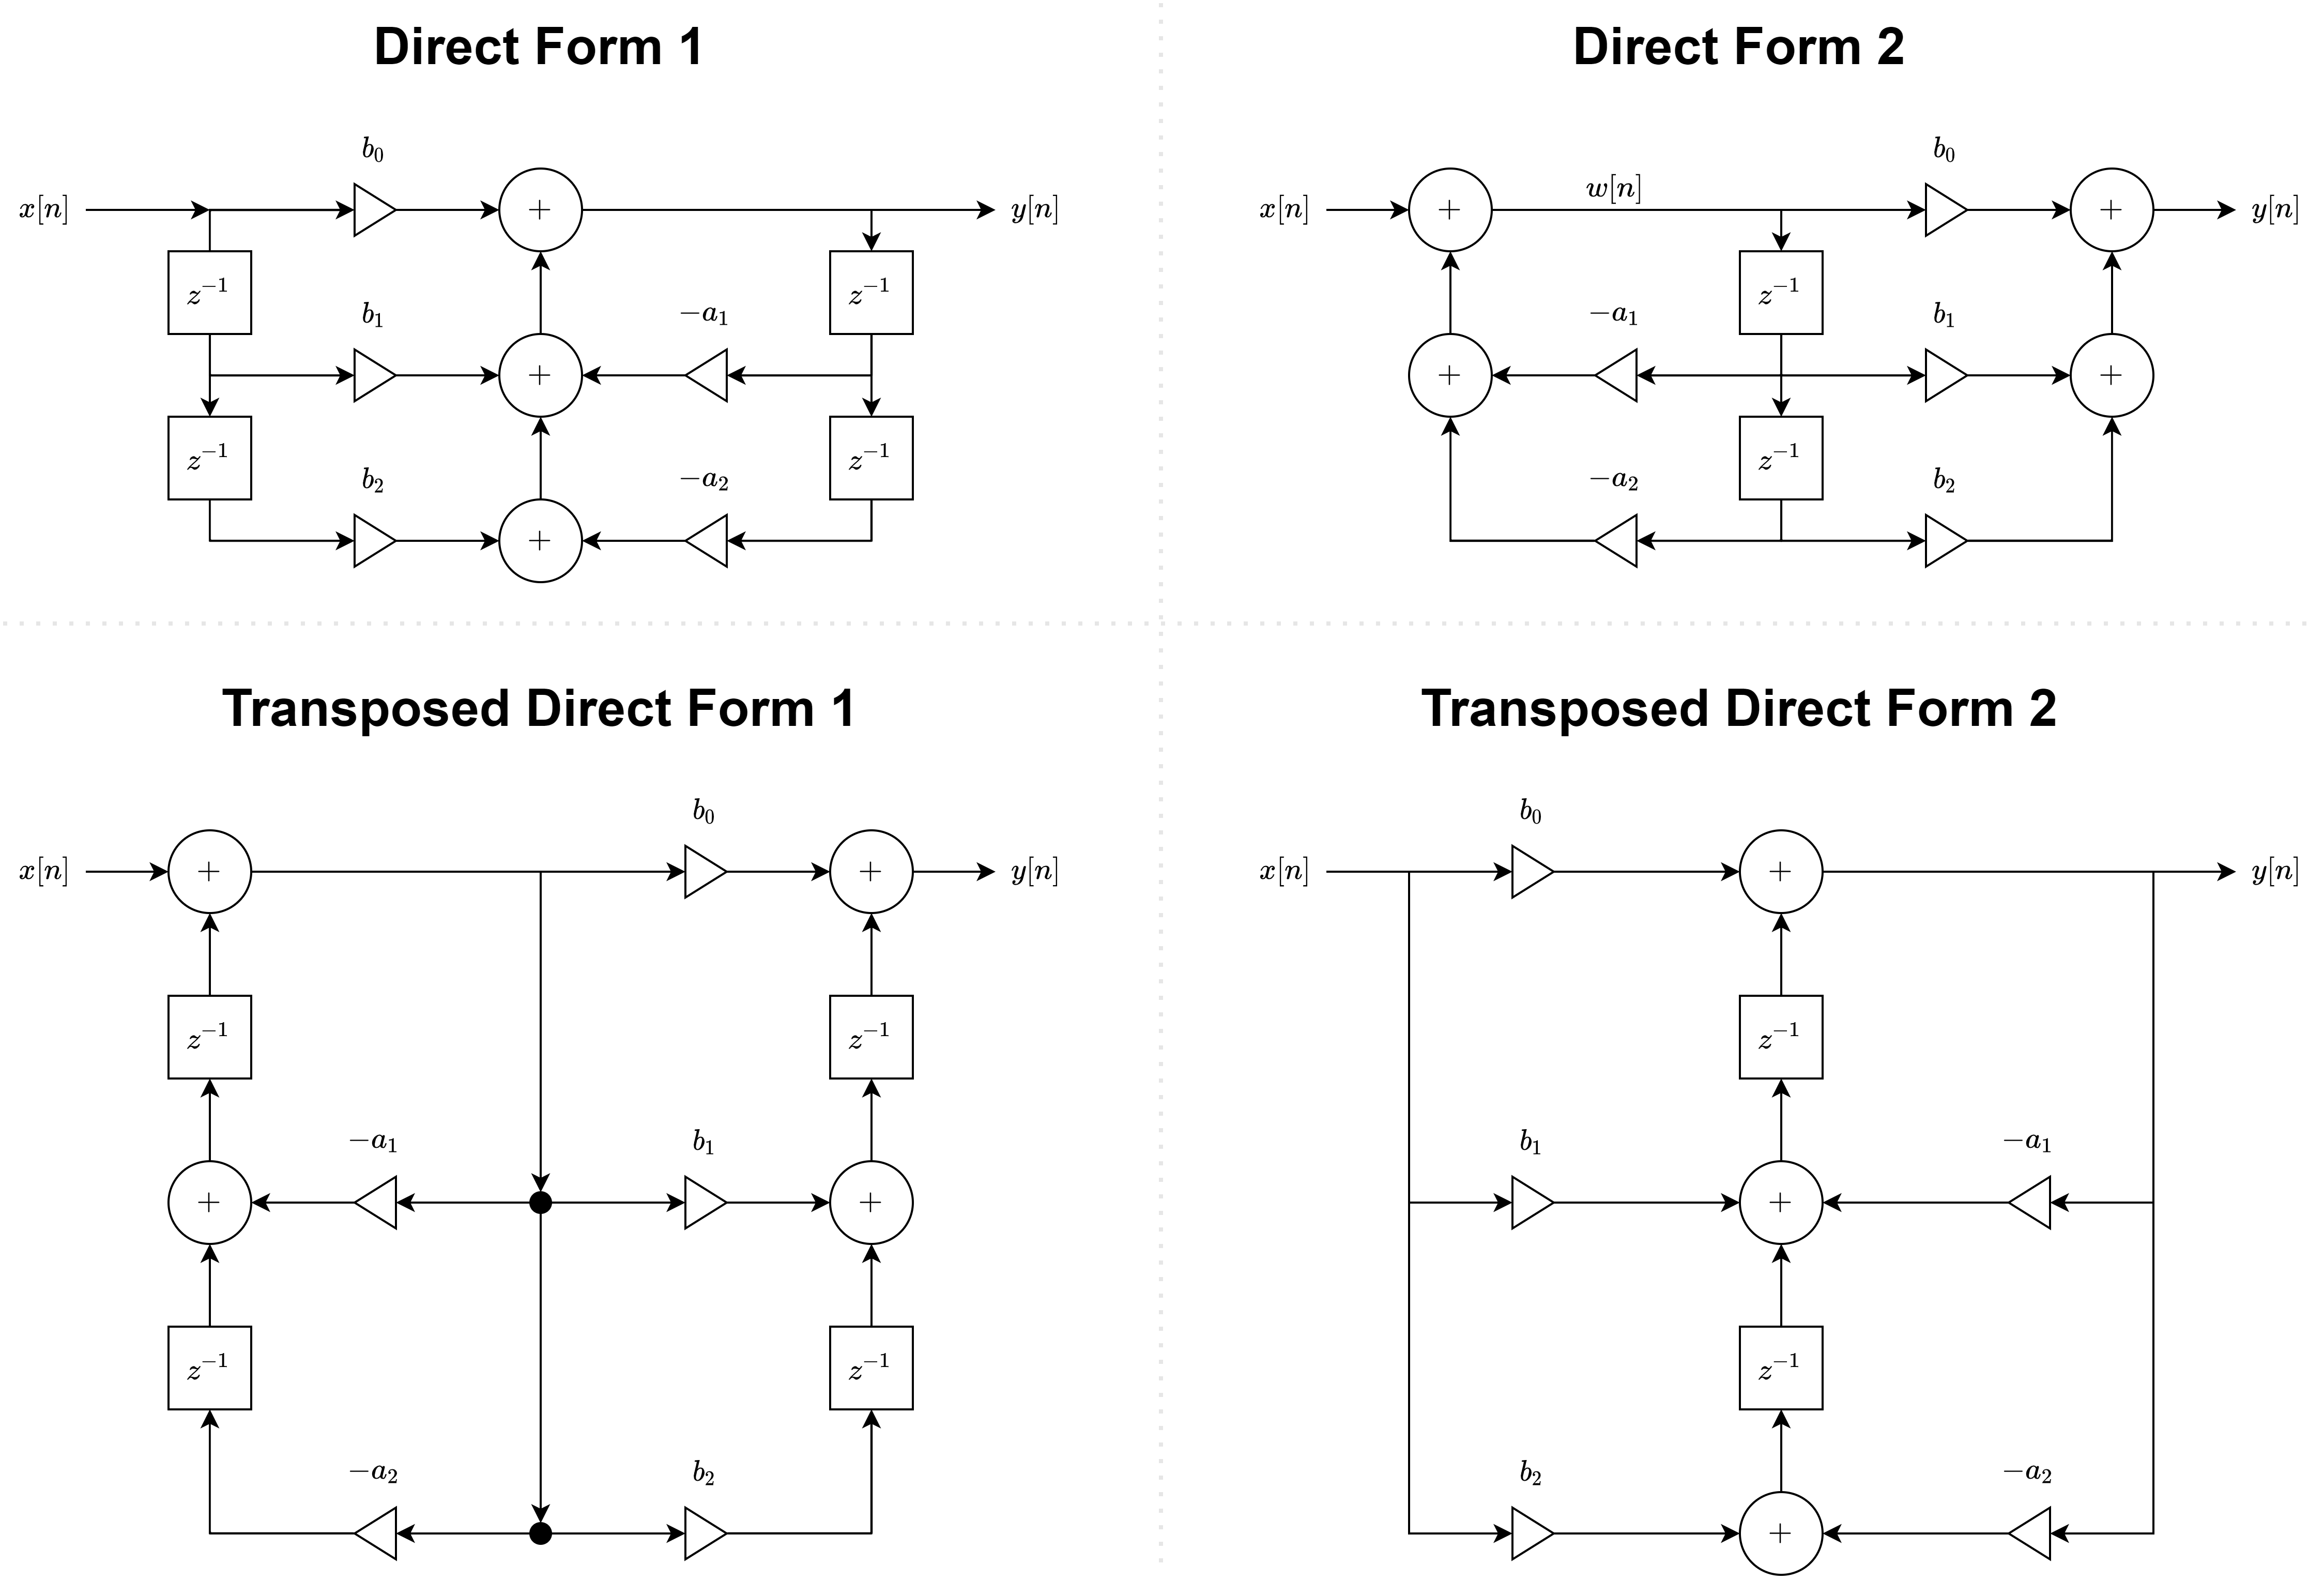
\includegraphics[width=1\linewidth]{images/BAT_BiQuad-Uebersicht}
		\caption{Übersicht BiQuad-Filter}
		\label{fig:batbiquad-uebersicht}
	\end{figure}
	\subsubsection*{PDM Clock}
	Das Mikrofon benötigt einen exakten Clock, um die PDM-Daten an den Mikrocontroller bzw. dessen PDM2PCM-Periphiere zu übertragen. Um das Mikrofon im "HIGH PERFORMANCE MODE" laufen lassen zu können, wird gemäss Datenblatt (\cite{noauthor_httpsinvensensetdkcomwp-contentuploads202007ds-000157-ics-41351-v14pdf_nodate}) ein Clock von 3.072MHz benötigt. Da dieser nicht direkt aus einem der bereits verfügbaren Clocks abgeleitet bzw. herunter- geteilt werden kann, muss dieser mittels dem integrierten PLL erzeugt werden. Der Prozess ist in Abbildung \ref{fig:batclock-muxing-pdm} ersichtlich, wobei der effektive PLL-Clock mittels der Formel \ref{eq:PLL-Formel} berechnet werden muss.
	\begin{equation}\label{eq:PLL-Formel}
		Frequenz_{PLL} = \underbrace{Frequenz_{ref}}_{LFXO} \cdot \frac{\overbrace{N+1}^{300\,<=\, N \, <= \, 4095}}{\underbrace{M+1}_{0\,<=\,M\,<=\,4095}}
	\end{equation}
	\begin{figure}[H]
		\centering
		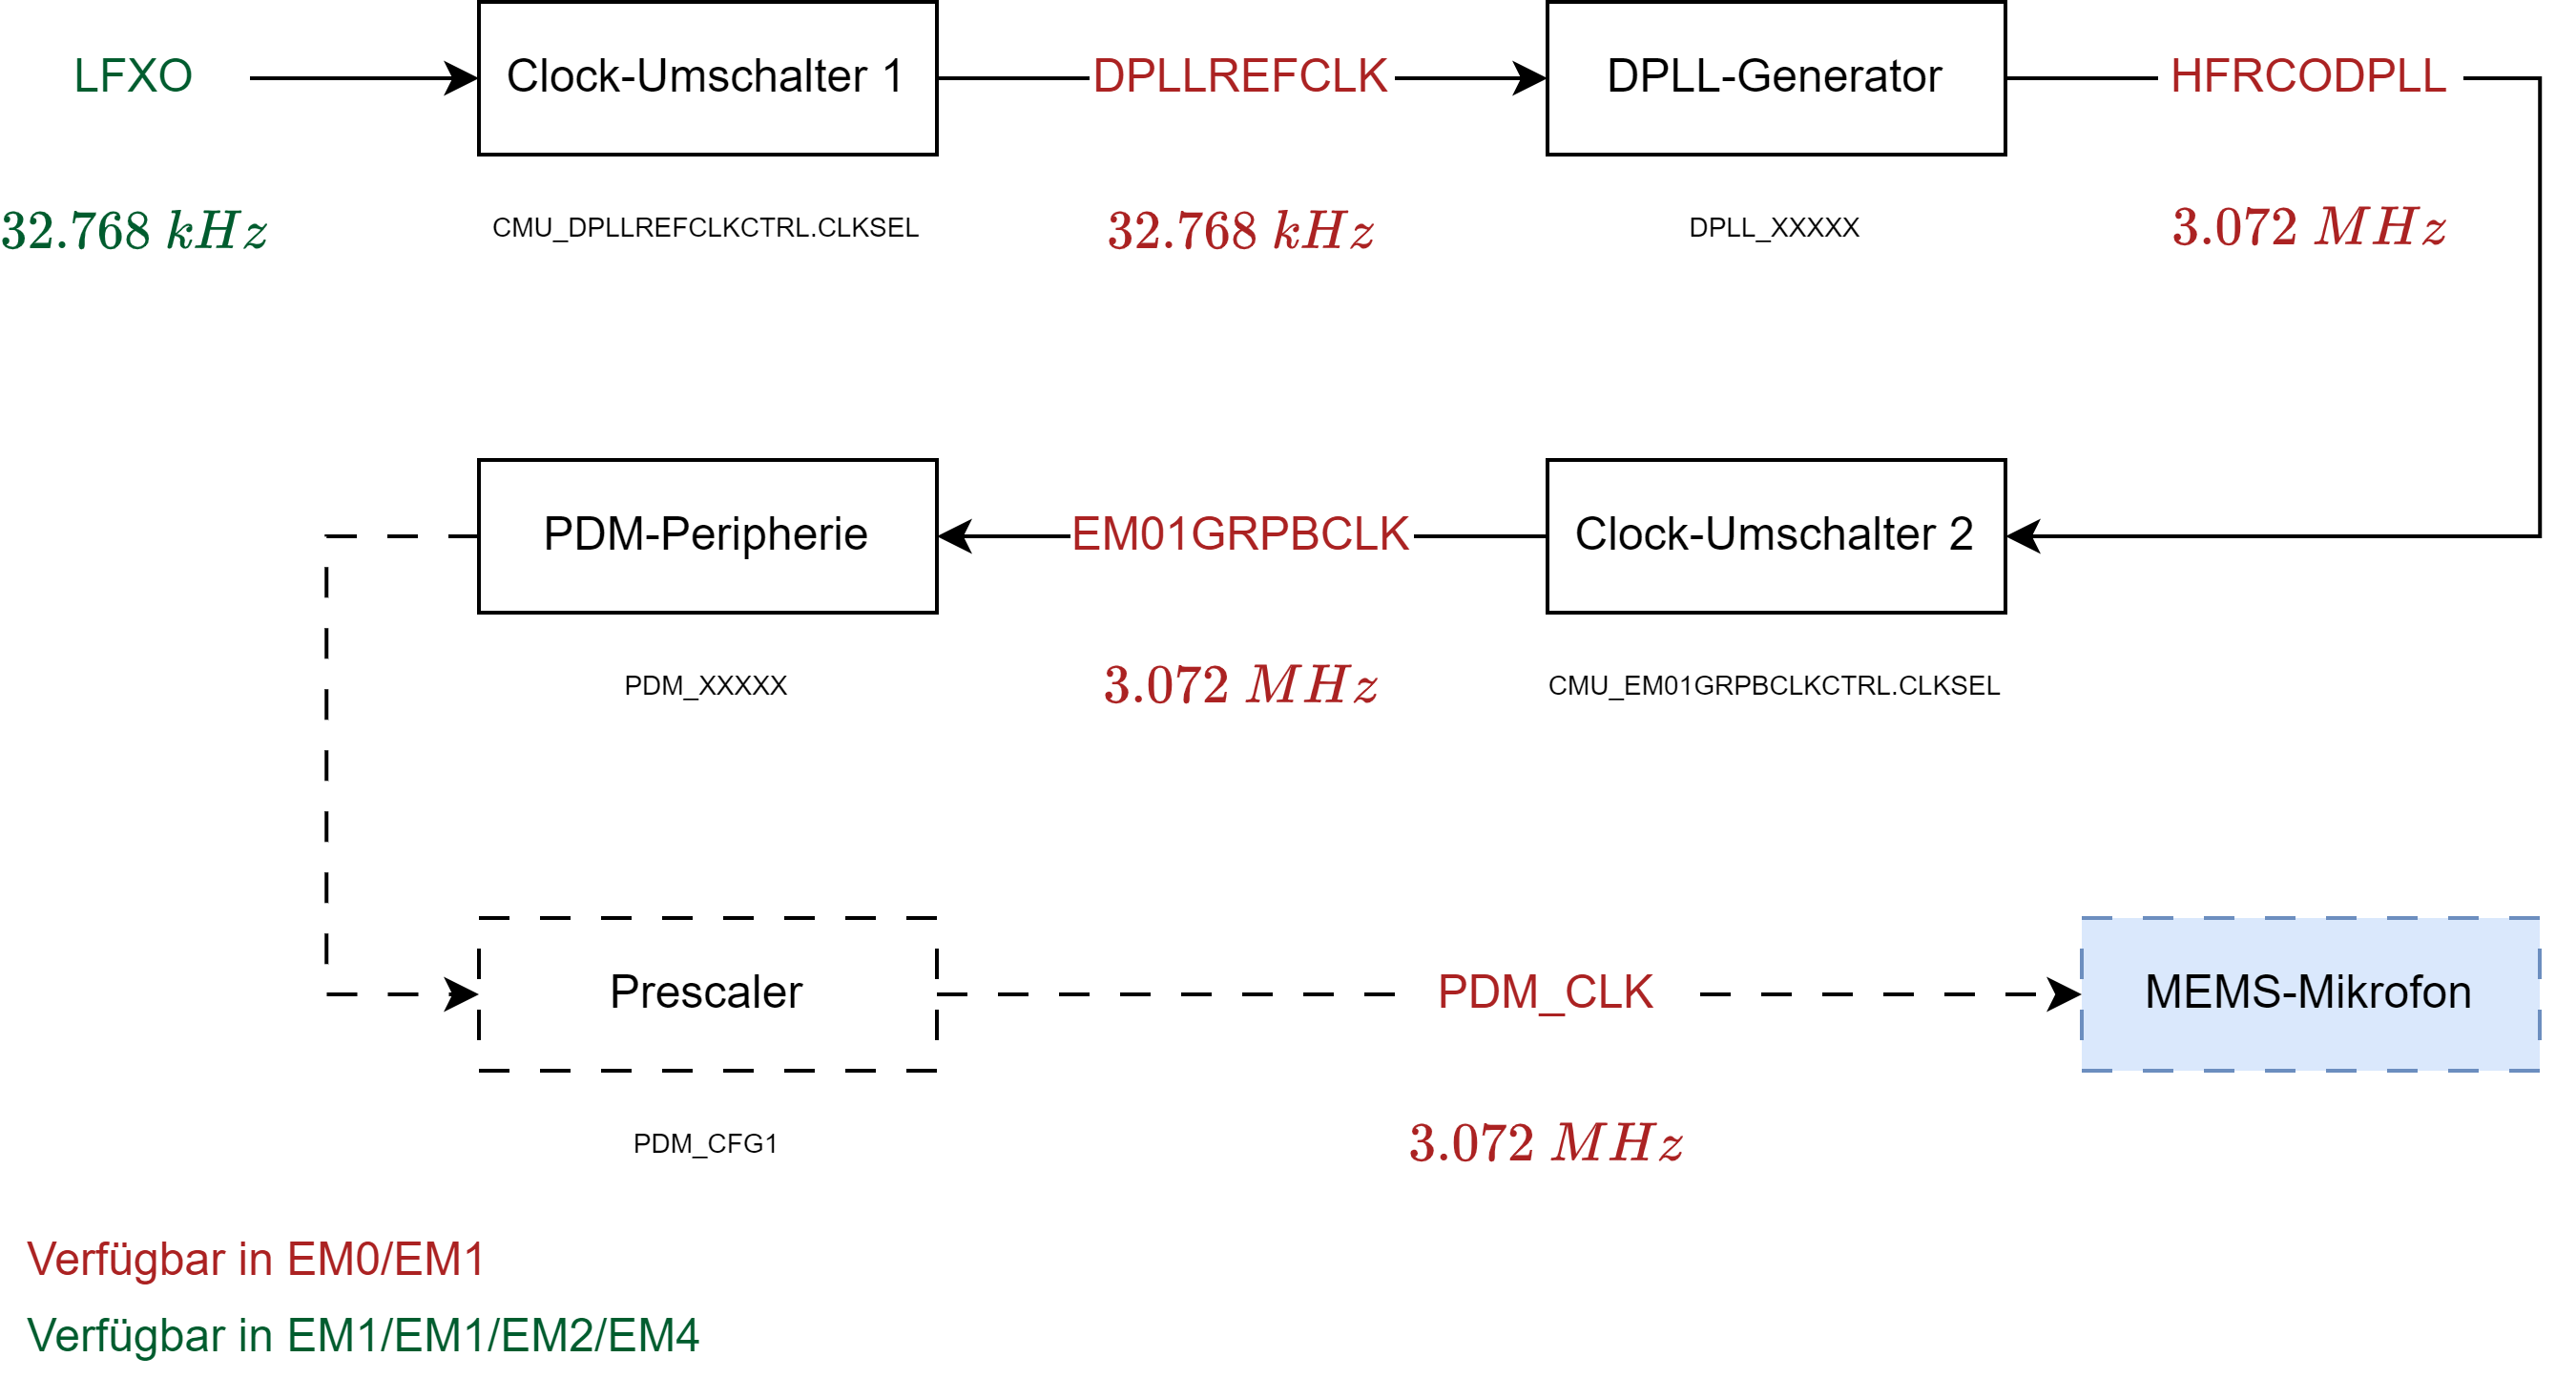
\includegraphics[width=1\linewidth]{images/BAT_Clock-Muxing-PDM}
		\caption{Clock-Muxing für 3.072MHz PDM}
		\label{fig:batclock-muxing-pdm}
	\end{figure}
	\subsubsection*{PDM CIC-Filter}
	Um aus dem 1-Bit PDM-Datenstream ein verarbeitbares PCM-Signal zu erhalten, wird die integrierte CIC-Filterstruktur verwendet. Gemäss \cite{silicon_efr32xg22_2022}, (\ref{fig:batpdmgrundbegriffe}) sowie \cite{noauthor_httpsinvensensetdkcomwp-contentuploads202007ds-000157-ics-41351-v14pdf_nodate} muss diese folgendermassen konfiguriert sein:
	\begin{itemize}[topsep=10pt,partopsep=0pt,labelwidth=5cm,align=left,itemindent=5cm]
	\item[$\bullet$ Dezimierungsrate:] 64
	\item[$\bullet$ Wortbreite:]  24 Bit
	\item[$\bullet$ Verstärkung (\ref{eq:Verstärkung}):]  0 dB 
	\item[$\bullet$ Filterordnung:]  5
	\item[$\bullet$ Clock-Dezimierung (\ref{eq:Clock-Dezimierung}):]  0 
	\item[$\bullet$ Abtastrate:]  48 kHz
	\end{itemize}
	\begin{equation}\label{eq:Clock-Dezimierung}
		Dezimierung = \frac{Taktfrequenz}{Abtastrate \cdot Dezimierungsrate} - 1
	\end{equation}
	\begin{equation}\label{eq:Verstärkung}
		Verst\ddot{a}rkung = 30 - ceil \left( \dfrac{log_{10}\left(Dezimierungsrate^{Filterordnung}\right)}{log_{10}(2)}\right)
	\end{equation}
	\subsubsection*{Schalldruckpegel}
	Wie in Abbildung \ref{fig:batfrequenzgewichtung} ersichtlich, durchläuft die Schalldruckpegel-Berechnung drei Phasen:
	\begin{itemize}
		\item Mittelwert $\vert$ Offset-Korrektur\\
		Das gemessene und gefilterte Signal ist in den meisten Fällen nicht mittelwertfrei. Dadurch beinhaltet dieses einen unbekannten Offset von der X-Achse. Um im Anschluss die Signalenergie sowie den dazugehörigen dB-Wert korrekt berechnen zu können, muss das Signal jedoch mittelwertfrei sein. Dazu wird die folgende Formel vor jeder Umrechnung angewendet:
		\begin{equation}\label{eq:Mittelwert}
			\bar{x} = \frac{1}{n}\sum_{i=1}^{n} Sample_i
		\end{equation}
		\item RMS $\vert$ Signalenergie \\
		Um aus dem mittelwertfreien Signal den dB-Wert berechnen zu können, muss zuvor die mittlere Signalenergie berechnet werden. Dies geschieht mit der nachfolgenden Formel:
		\begin{equation}\label{eq:RMS}
			x_{RMS} = \sqrt{\frac{1}{n}\sum_{i=1}^{n} \left( Sample_i-\bar{x}\right)^2}
		\end{equation}\blfootnote{n = Anzahl gemessene Samples}
		\item dB-Umwandlung\\
		Zur effektiven Berechnung des Schalldruckpegels muss die allgemein gültige Formel aus der Theorie (\ref{eq:dBSPL}) mit den maximalen Messwerten erweitert werden. Gleichzeitig wird der Referenz-Schalldruckpegel $P_0$ durch den maximalen, digitalen Wert, $dBFS$, ersetzt. Daraus entsteht folgende, finale Formel:
		\begin{equation}\label{eq:dBSPL2}
			dBSPL = \underbrace{129.5dB}_{AOP \, \cite{noauthor_httpsinvensensetdkcomwp-contentuploads202007ds-000157-ics-41351-v14pdf_nodate}} + 20 \cdot log_{10}\left( \frac{x_{RMS}}{8388607}\right) 
		\end{equation}\blfootnote{dBFS = $\frac{2^{Aufl\ddot{o}sung}}{2}$}
	\end{itemize}
	\subsubsection*{I²C}
	\begin{figure}[H]
		\centering
		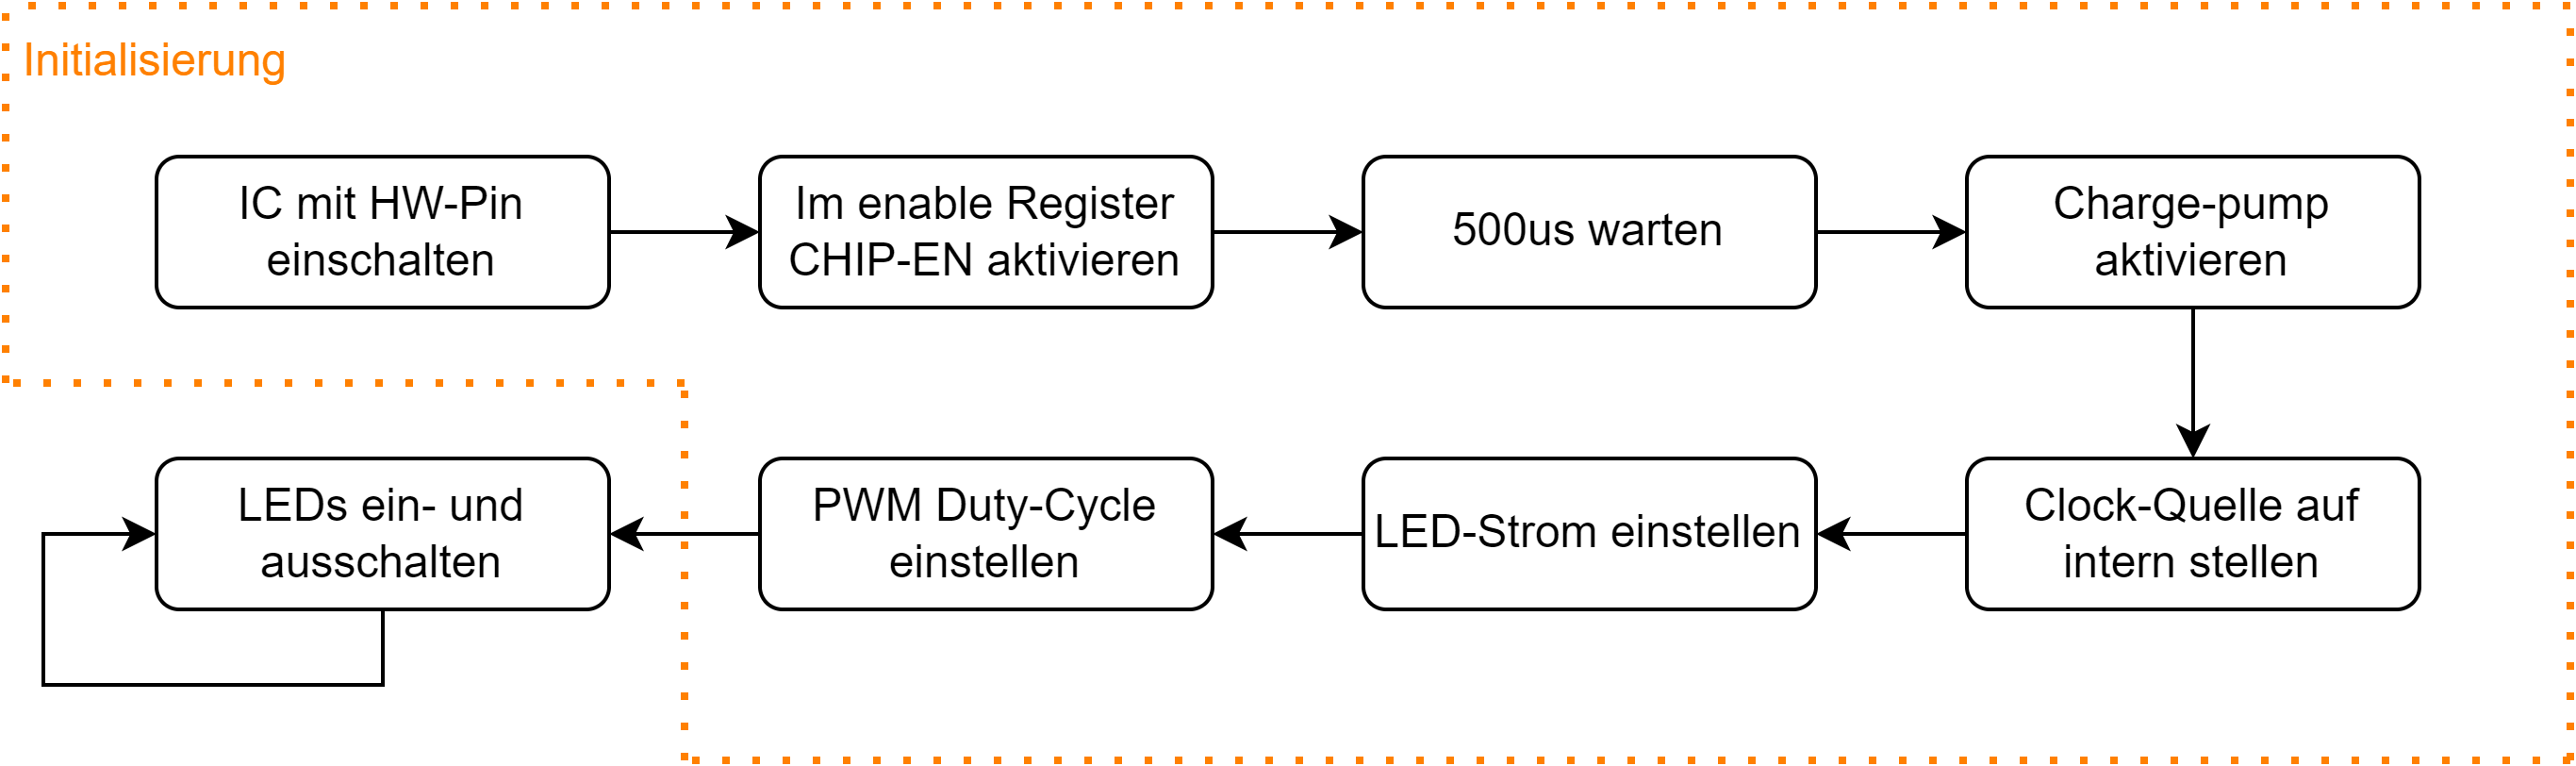
\includegraphics[width=1\linewidth]{images/BAT_Flussdiagramm_I2C_V2}
		\caption{Softwareablauf I²C}
		\label{fig:batflussdiagrammi2cv2}
	\end{figure}
	\subsubsection*{SPI}
	Da der SPI-Treiber hauptsächlich mittels der SPIDRV-Bibliothek von Silicon Labs implementiert ist, fällt der Treiber schlank aus. Es existieren lediglich jeweils eine Funktion um eine neue Seite (512 Bytes) im Speicher zu beschreiben und um diese auch wieder auszulesen bzw. zu löschen.
	\subsubsection*{RTC}
	Die RTC wird, im Gegensatz zur restlichen Peripherie, nicht selbst aufgesetzt und betrieben. Dies ist darauf zurückzuführen, dass der BLE-Stack von Silicon Labs zum Zeitmanagement denselben Zeitgeber verwendet. Dadurch ist der Zugriff auf die RTC limitiert und kann nur über die nachfolgende Funktion abgerufen werden:
	$$ sl\_sleeptimer\_get\_time() $$
	Dabei wird die Zeit auf die Sekunde genau zurückgegeben und kann somit für die Erzeugung des Zeitstempels verwendet werden.
	\subsubsection*{LEDs} \label{LEDs}
	Auf Wunsch des Industriepartners werden die SPL-Werte so auf die 8 LEDs abgebildet, dass der 85dB(A)-Wert auf LED 4 zu liegen kommt mit jeweils einer Veränderung von $\pm$ 3dB(A) auf die nachfolgenden LEDs. Dabei entspricht ein Schritt von +3dB, gemäss Formel \ref{eq:dBSPL}, einer Lautstärkeverdoppe\-lung. Somit sieht die momentane Skalierung folgendermassen aus:
	\begin{figure}[H]
		\centering
		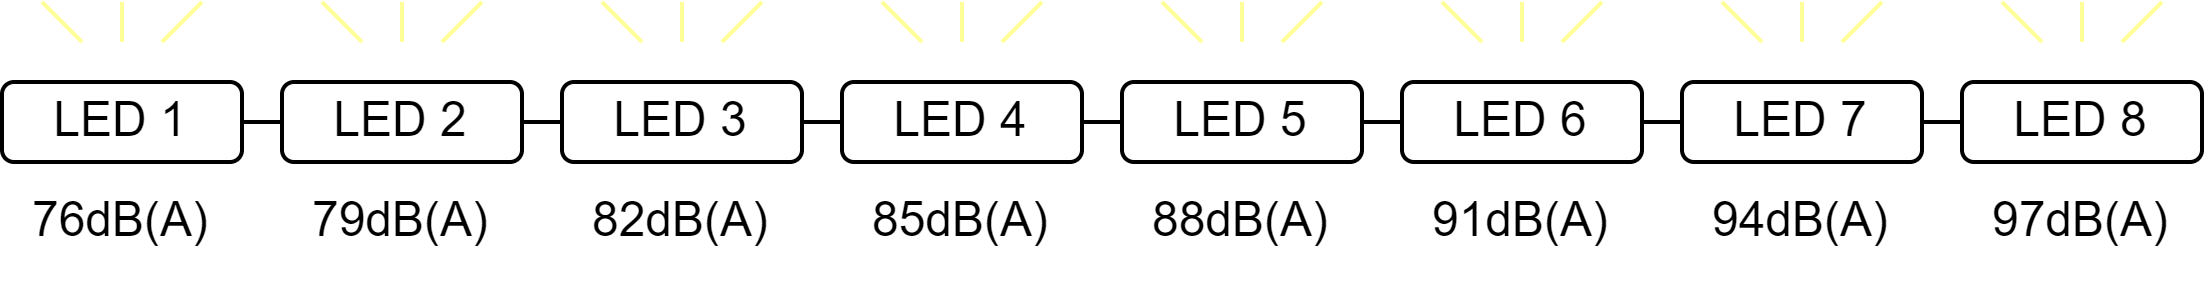
\includegraphics[width=1\linewidth]{images/BAT_Skalierung-SPL-auf-LED}
		\caption{Aufteilung dBSPL auf 8 LEDs}
		\label{fig:batskalierung-spl-auf-led}
	\end{figure}
	
	
	\newpage
	\section{Messungen}\label{Messungen}
	Ein System kann qualitativ nur mit Messungen auf seine Einsatzfähigkeit untersucht werden. Dadurch erfolgen nachfolgend theoretische und praktische Messwerte.
	\subsection{Ausführungsgeschwindigkeit}
	Um die Dauer einer Funktion messen zu können, wurde ein GPIO-Pin zu Beginn sowie am Ende der jeweiligen Funktion umgeschaltet und mit den Logic-Analyzer ausgewertet. Aus 20 Funktionsaufrufen wurde anschliessend der Mittelwert berechnet und in Tabelle \ref{tab:ausfuehrungsgeschwindigkeit} aufgeführt. \\
	Die Messungen zeigen, dass hauptsächlich das Messen der Werte, sowie die Filterung dieser, die meiste Zeit in Anspruch nimmt. Gleichzeitig kann jedoch so verifiziert werden, dass ein Messintervall von 125ms (Messmodus: Fast) möglich ist.
	\begin{table}[H]
		\centering
		\begin{tabular}{|l|l|l|}
			\hline
			\textbf{Funktionsname} & \textbf{Zeit [ms]} & \textbf{Bemerkung} \\ \hline
			app\_init & 10.4 & RTC, SPI, I2C, PDM, \\ 
			 ~ & ~ & Timer, GPIO \\ 
			 \hline
			PDM\_readMicrophone & 20.8 & 128 Samples; Low-Power \\ \hline
			RTC\_convertTimeToString & 0.16 & Format: 00:00:00 \\ \hline
			PDM\_applyAWeightingFilter & 15.2 & 128 Samples \\ \hline
			PDM\_convertPCMTodBSPL & 0.81 & 128 Samples \\ \hline
			PDM\_convertSPLToString & 0.28 & ~ \\ \hline
			I2C\_enableLedRange & 0.62 & ~ \\ \hline
			LOGGING\_generateLogString & 0.01 & Länge: 13 char \\ \hline
			SPI\_writePage / SPI\_readPage & 4.4 & 512 Bytes \\ \hline
			~ & ~ & ~ \\ \hline
			Total & 52.68 ms & ~ \\ \hline
			Total pro Messintervall & \textbf{42.28} ms & ~ \\ \hline
		\end{tabular}
		\caption{Ausführungsgeschwindigkeit der einzelnen Funktionen}
		\label{tab:ausfuehrungsgeschwindigkeit}
	\end{table}
	\subsection{Energieaufnahme}
	Die Energieaufnahme eines Systems zu quantifizieren, stellt sich als durchaus komplex dar. Viele Variablen, Abwägung von Verarbeitungsgeschwindigkeit mit der gegensätzlichen Energieeffizienz und nicht genau spezifizierte Parameter erschweren die Festlegung der Rahmenbedingungen. Bei der Auslegung der nachfolgenden Parameter wird stets die energieeffizienteste Möglichkeit gewählt, ohne damit die Leistungsfähigkeit massgeblich zu beeinflussen.
	\paragraph{Mikrocontroller}\mbox{}\\
	Die Energieaufnahme des Mikrocontrollers ist nicht nur von der eigentlichen Taktrate abhängig, sondern auch welche Peripherieblöcke und Low-Power-Modi gerade aktiv sind. Dadurch lässt sich die Energieaufnahme nur sehr grob abschätzen. Mit den benötigten Peripherien aktiv, jedoch ohne eine Berechnung durchzuführen und in einen Low-Power-Modus zu wechseln, könnte die Energieaufnahme folgendermassen aussehen:
	\begin{equation}\label{eq:Leistung_Mikrocontroller_basic}
		\approx \underbrace{27 \mu A/MHz \cdot 76.8MHz}_{ \mu C} + \underbrace{10 \mu A/MHz \cdot 76.8MHz}_{Peripherie} = 2842 \mu Ah
	\end{equation}
	\paragraph{Mikrofon}\mbox{}\\
	Wie der Formel \ref{eq:Leistung_Mikrofon} entnommen werden kann, gibt es zwei Möglichkeiten das Mikrofon zu verwenden:
	\begin{itemize}
		\item Das Mikrofon wird konstant im Performance-Modus betrieben. Durch den Einsatz von DMA sind die benötigten Messewerte jeder Zeit verfüg\-bar und die 20ms Startzeit des Mikrofons entfällt. Dadurch sind höher aufgelöste Messintervalle möglich. Dazu sind die Messungen der einzelnen Funktionen in Tabelle \ref{tab:ausfuehrungsgeschwindigkeit} ersichtlich.
		\item Das Mikrofon wird nur dann aktiviert, wenn es benötigt wird. Dadurch sinkt die benötigte Leistung von 580$\mu Ah$ auf 87.2 $\mu Ah$ (\ref{eq:Leistung_Mikrofon}). In der Folge erhöht sich die benötigte Messzeit um 20ms. Dies aus dem Grund, dass keine DMA verwendet wird und das Mikrofon vom Standby-Betrieb (20 $\mu A$) in den Performance-Modus (580 $\mu A$) wechselt.
	\end{itemize}
	\begin{equation}\label{eq:Leistung_Mikrofon}
		Leistung_{Mikrofon} \approx \underbrace{580 \mu A \cdot 120ms }_{ Performance-Modus} + \underbrace{20 \mu A \cdot 880ms}_{Standby} = 87.2 \mu Ah
	\end{equation}
	\paragraph{EEPROM}\mbox{}\\
	Der Chip weist eine Vielzahl von unterschiedlichen Leistungsmodi auf. Die Energieaufnahme variiert zwischen dem niedrigen Standby-Modus (35$\mu Ah$) und dem Schreiben einer Seite (3$mAh$) von 512 Bytes. Gemäss folgender Mischrechnung (\ref{eq:Leistung_EEPROM}) kann die ungefähre Energieaufnahme approximiert werden.
	\begin{equation}\label{eq:Leistung_EEPROM}
		\approx \underbrace{3mA \cdot 4.5ms}_{Schreiben} + \underbrace{1.5mA \cdot 2ms}_{Lesen} +  \underbrace{35\mu A \cdot 993.5ms}_{Standby}= 51.3 \mu Ah\footnote{Alle Zeiten gemäss Datenblatt}
	\end{equation}
	\paragraph{Übersicht berechnet}\mbox{}\\
		\begin{table}[H] 
			\vspace*{-0.5cm}
			\centering
			\begin{tabular}{|l|l|l|}
			\hline
			\textbf{Bauteil} & \textbf{Strom} & \textbf{Bemerkung} \\ \hline
			Mikrocontroller & 2842 $\mu Ah$ & ~ \\ \hline
			LEDs & 800 $\mu Ah$ & 100$\mu Ah$ pro LED $\cdot$ 8 LEDs \\ \hline
			LED-Treiber & 600 $\mu Ah$ & Alle Ausgänge EIN \\ \hline
			EEPROM & 51.3 $\mu Ah$ & ~ \\ \hline
			Mikrofon & 87.2 $\mu Ah$ & Low-Power-Modus \\ \hline
			~ & ~ & ~ \\ \hline
			Total & 4.4 $mAh$ & ~ \\ \hline
			Total Arbeitstag à 12h & \textbf{52.6} $mAh$ & ~ \\ \hline
		\end{tabular}
		\caption{Berechnete Energieaufnahme des Gesamtsystems}
		\label{tab:leistung-berechnet}
	\end{table}
	\paragraph{Übersicht gemessen}\mbox{}\\
		\begin{table}[H] 
			\vspace*{-0.5cm}
			\centering
			\begin{tabular}{|l|l|l|}
			\hline
			\textbf{Bauteil} & \textbf{Strom} & \textbf{Bemerkung} \\ \hline
			Mikrocontroller & 1760 $\mu Ah$ & Alle Peripherien EIN \\ \hline
			LEDs & 780 $\mu Ah$ & Alle LEDs EIN\\ \hline
			LED-Treiber & 820 $\mu Ah$ & Alle Ausgänge EIN \\ \hline
			EEPROM & 70 $\mu Ah$ & ~ \\ \hline
			Mikrofon & 103 $\mu Ah$ & Messintervall: 250ms \\ \hline
			~ & ~ & ~ \\ \hline
			Total & 3.5 $mAh$ & ~ \\ \hline
			Total Arbeitstag à 12h & \textbf{42.40} $mAh$ & ~ \\ \hline
		\end{tabular}
		\caption{Gemessene Energieaufnahme des Gesamtsystems}
		\label{tab:leistung-gemessen}
		\end{table}
	\noindent Wie insbesondere der Tabelle \ref{tab:leistung-gemessen} zu entnehmen ist, kann die Einsatzdauer von 12 Stunden mit einem 50mAh-Akku abgedeckt werden.
	\subsection{Mikrofon-Messungen} \label{Mikrofon-Messungen}
	Das MEMS-Mikrofon, sowie das M2211 von NTI, wurden beide jeweils vor jeder Messung mittels dem CAL200 auf 94dBSPL kalibriert. Da die Abstände zwischen den Mikrofonen und dem CAL200 nicht identisch sind, wurden zudem noch eine Feinkalibrierung durchgeführt. Genauere Angaben dazu sind dem Anhang \hyperref[Messmittel]{Messmittel} sowie \hyperref[Kalibrationsmessung]{Kalibrationsmessung} zu entnehmen.
	\paragraph{Messaufbau SPL}
		\begin{itemize}[topsep=10pt,partopsep=0pt,labelwidth=5cm,align=left,itemindent=5cm]
		\item[$\bullet$ Messfrequenz:] 1 kHz
		\item[$\bullet$ Amplitude:]  1 Vrms
		\item[$\bullet$ Signalform:]  Sinus
		\item[$\bullet$ Gewichtung:]  Z
		\item[$\bullet$ Distanz zu Signalquelle:]  100 mm ... 800 mm
		\item[$\bullet$ Zeitgewichtung:]  Slow
		\item[$\bullet$ Visualisierung:]  \ref{fig:messaufbau_spl}
	\end{itemize}
	\paragraph{Messaufbau Frequenzgang}
		\begin{itemize}[topsep=10pt,partopsep=0pt,labelwidth=5cm,align=left,itemindent=5cm]
			\item[$\bullet$ Messfrequenz:] 10 Hz ... 20 kHz
			\item[$\bullet$ Amplitude:]  1 Vrms
			\item[$\bullet$ Signalform:]  Sinus
			\item[$\bullet$ Gewichtung:]  A, C, Z
			\item[$\bullet$ Zeitgewichtung:]  Slow
			\item[$\bullet$ Distanz zu Signalquelle:]  200 mm
			\item[$\bullet$ Visualisierung:]  \ref{fig:messaufbau_frequenzgang}
		\end{itemize}
	\begin{figure}[H]
		\centering
		\begin{tikzpicture}
			\begin{axis}[
				width=1\textwidth,
				xmode=log,
				title={\textbf{dB(Z)}},
				xlabel={Frequenz [Hz]},
				ylabel={Schalldruckpegel [dB]},
				xmin=50, xmax=20000,
				ymin=50, ymax=100,
				legend pos=north west,
				xminorgrids=true,
				xmajorgrids=true,
				ymajorgrids=true,
				grid style=dashed,
				]
				\addplot[
				smooth,
				color=blue,
				mark=solid,
				] table[col sep=semicolon, x=Frequenz, y=MEMS_Z_2] {measurements/Microphone/BAT_Frequenzmessung_Geraet.csv};
				\addlegendentry{MEMS}
				\addplot[
				smooth,
				color=red,
				mark=solid,
				] table[col sep=semicolon, x=Frequenz, y=Referenz_Z_2] {measurements/Microphone/BAT_Frequenzmessung_Referenz.csv};
				\addlegendentry{M2211}
				\fill[yellow, opacity=0.3] (axis cs:2000, 0) -- (axis cs:20000, 0) -- (axis cs:20000, 120) -- (axis cs:2000, 120);
			\end{axis}
		\end{tikzpicture}
		\caption{Frequenz vs. Schalldruckpegel-Plot der ungewichteten Messung $\vert$ dB(Z)}
		\label{fig:microphone_plot_ungewichtet}
		\end{figure}
		Wie in Abbildung \ref{fig:microphone_plot_ungewichtet} ersichtlich, kann die Messung grob in zwei Bereiche eingeteilt werden:
		\begin{itemize}
			\item Bereich zwischen 50Hz und 2kHz \\
			Dieser ist unproblematisch, da er die Kennlinie des Referenzmikrofons widerspiegelt. Die vorhandenen Nichtlinearitäten sind auf den verwendeten Messlautsprecher sowie den dazugehörigen Verstärker zurückzuführen.
			\item \color{orange} Bereich grösser als 2kHz \color{black} \\
			Auch hier folgen die beiden Mikrofone der Nichtlinearität des Messaufbaus. Jedoch reagiert das \color{blue}MEMS\color{black}-Mikrofon sensitiver auf diesen Frequenzbereich, als das Referenzprodukt. Dieses Phänomen ist auf den Helmholtz Effekt zurückzuführen. Dieser tritt, bauartbedingt, ab einer gewissen Frequenz bei allen MEMS-Mikrofonen auf. Ersichtlich ist dieser in \cite{noauthor_httpsinvensensetdkcomwp-contentuploads202007ds-000157-ics-41351-v14pdf_nodate}, Abbildung 4. Dabei schwingt das Mikrofongehäuse mit der Membrane mit (wobei eine gewisse Resonanz entsteht) und erzeugt somit einen höheren Schalldruck.
		\end{itemize}
		
		\begin{figure}[H]
		\centering
			\begin{tikzpicture}
				\begin{axis}[
					width=1\textwidth,
					xmode=log,
					title={\textbf{dB(A)}},
					xlabel={Frequenz [Hz]},
					ylabel={Schalldruckpegel [dB]},
					xmin=50, xmax=20000,
					ymin=50, ymax=100,
					legend pos=north west,
					xminorgrids=true,
					xmajorgrids=true,
					ymajorgrids=true,
					grid style=dashed,
					]
					\addplot[
					smooth,
					color=blue,
					mark=solid,
					] table[col sep=semicolon, x=Frequenz, y=MEMS_A_3] {measurements/Microphone/BAT_Frequenzmessung_Geraet.csv};
					\addlegendentry{MEMS}
					\addplot[
					smooth,
					color=red,
					mark=solid,
					] table[col sep=semicolon, x=Frequenz, y=Referenz_A_2] {measurements/Microphone/BAT_Frequenzmessung_Referenz.csv};
					\addlegendentry{M2211}
					\addplot[
					smooth,
					color=green,
					mark=solid,
					dashed,
					] table[col sep=semicolon, x=Frequenz, y=Kurve_A] {measurements/Microphone/BAT_Frequenzmessung_Geraet.csv};
					\addlegendentry{Referenz}
				\end{axis}
			\end{tikzpicture}
			\caption{Frequenz vs. Schalldruckpegel-Plot der gewichteten Messung $\vert$ dB(A)}
			\label{fig:microphone_plot_gewichtet_A}
		\end{figure} 
		\noindent Wie in Abbildung  \ref{fig:microphone_plot_gewichtet_A} aufgezeigt, werden die Frequenzen bis ca. 1kHz gedämpft. Dies entspricht der Filtercharakteristik, welche in Abbildung \ref{fig:frequenzbewertung} ersichtlich ist. Somit kann bestätigt werden, dass der implementierte Filter funktioniert.
		\begin{figure}[H]
		\centering
			\begin{tikzpicture}
				\begin{axis}[
					width=1\textwidth,
					xmode=log,
					title={\textbf{dB(C)}},
					xlabel={Frequenz [Hz]},
					ylabel={Schalldruckpegel [dB]},
					xmin=50, xmax=20000,
					ymin=50, ymax=100,
					legend pos=north west,
					xminorgrids=true,
					xmajorgrids=true,
					ymajorgrids=true,
					grid style=dashed,
					]
					\addplot[
					smooth,
					color=blue,
					mark=solid,
					] table[col sep=semicolon, x=Frequenz, y=MEMS_C_2] {measurements/Microphone/BAT_Frequenzmessung_Geraet.csv};
					\addlegendentry{MEMS}
					\addplot[
					smooth,
					color=red,
					mark=solid,
					] table[col sep=semicolon, x=Frequenz, y=Referenz_C_2] {measurements/Microphone/BAT_Frequenzmessung_Referenz.csv};
					\addlegendentry{M2211}
					\addplot[
					smooth,
					color=green,
					mark=solid,
					dashed,
					] table[col sep=semicolon, x=Frequenz, y=Kurve_C] {measurements/Microphone/BAT_Frequenzmessung_Geraet.csv};
					\addlegendentry{Referenz}
				\end{axis}
			\end{tikzpicture}
			\caption{Frequenz vs. Schalldruckpegel-Plot der gewichteten Messung $\vert$ dB(C)}
			\label{fig:microphone_plot_gewichtet_C}
		\end{figure}
		\noindent Auch der in Abbildung  \ref{fig:microphone_plot_gewichtet_C} gezeigte Frequenzgang repräsentiert den erfolgreich umgesetzten C-Gewichtungsfilter. Dabei werden die hohen Frequenzen etwas stärker gedämpft als beim dB(A)-Filter. Als Referenz dient auch hier die Abbildung \ref{fig:frequenzbewertung}.
		\begin{figure}[H]
		\centering
			\begin{tikzpicture}
				\begin{axis}[
					width=1\textwidth,
					xmode=linear,
					title={\textbf{Abstandsmessung}},
					xlabel={Distanz zu Schallquelle [mm]},
					ylabel={Schalldruckpegel [dB]},
					xmin=100, xmax=800,
					ymin=60, ymax=100,
					legend pos=north west,
					ymajorgrids=true,
					grid style=dashed,
					]
					\addplot[
					color=blue,
					mark=solid,
					] table[col sep=semicolon, x=Distanz, y=MEMS] {measurements/Microphone/BAT_Frequenzmessung_Distanz.csv};
					\addlegendentry{MEMS}
					\addplot[
					color=red,
					mark=solid,
					] table[col sep=semicolon, x=Distanz, y=Referenz] {measurements/Microphone/BAT_Frequenzmessung_Distanz.csv};
					\addlegendentry{M2211}
					\addplot[
					dashed,
					color=green,
					mark=solid,
					] table[col sep=semicolon, x=Distanz, y=1/r] {measurements/Microphone/BAT_Frequenzmessung_Distanz.csv};
					\addlegendentry{1/r}
				\end{axis}
			\end{tikzpicture}
			\caption{Distanz vs. Schalldruckpegel-Plot}
			\label{fig:microphone_plot_distanz}
		\end{figure}
	\noindent Abbildung \ref{fig:microphone_plot_distanz} zeigt, dass nach der initialen Kalibration (siehe Anhang \ref{Kalibrationsmessung}) der Schalldruckpegel keine Abweichung vom Referenzgerät erfährt. Somit kann bestätigt werden, dass das Mikrofon sich bei abnehmender Distanz, im Vergleich zum XL2, gleich verhält. Zudem ist das reziproke Abstandsgesetz (\color{green}1/r\color{black}) in den Messwerten ersichtlich. Gemäss diesem sinkt der Schalldruckpegel bei doppelter Distanz um den Faktor 6.021dB und wird gemäss folgender Formel berechnet:
	\begin{equation}\label{eq:Abstandsgesetz}
		dB_{neu} = dB_{Ref} - 20 \cdot log_{10}\left( \frac{Abstand_{neu}}{Abstand_{ref}}\right) 
	\end{equation}
	
	\newpage
	\section{Validieren der Anforderungen} \label{Validierung}
	Die im Kapitel \ref{Ziele} definierten Ziele können nun anhand der Arbeit validiert werden.
	\begin{itemize}
		\item [\greencheck] Die Laufzeit des Gerätes soll mindestens 12 Stunden betragen. \\
		\textcolor{gray}{Gemäss Unterkapitel \ref{tab:leistung-gemessen} reicht ein 50mAh-Akku, um das Gerät während 12 Stunden betreiben zu können. Momentan verbaut ist ein 200mAh-Akku.}
		\item [\greencheck] Das Gerät wird mit einem Akku betrieben. Dieser wird via eines USB-C-Anschlusses aufgeladen. \\
		\textcolor{gray}{Das Gerät verfügt über einen Li-Io-Akku sowie einen power-only USB-C Anschluss. Siehe Kapitel \ref{Konzept}.}
		\item [\greencheck] Der Schalldruckpegel wird mit einem MEMS-Mikrofon aufgezeichnet. \\
		\textcolor{gray}{Dazu wird das ICS-41351 von TDK eingesetzt. Siehe Kapitel \ref{Mikrofon}.}
		\item [\greencheck] Die Messdaten werden in regelmässigen Abständen auf dem Gerät gespeichert. \\
		\textcolor{gray}{Das Messintervall kann über das Define angepasst werden. Siehe Kapitel \ref{Timer}.}
		\item [\greencheck] Das Gerät verfügt über eine BLE-Schnittstelle, um die Messdaten drahtlos an ein Zielgerät zu übertragen.\\
		\textcolor{gray}{Der Mikrocontroller ist zur Datenübertragung vorbereitet. Siehe Kapitel \ref{Konzept}.}
		\item [\greencheck] Der aktuelle Schalldruckpegel wird auf der Vorderseite des Gerätes visuell dargestellt. \\
		\textcolor{gray}{Es befinden sich 8 LEDs auf der Vorderseite des Gerätes, welche in \\ $\pm$ 3dB Abständen den Schalldruckpegel anzeigen. Siehe Kapitel \ref{LEDs}.}
		\item [\greencheck] Die Bauform der Platine fällt rund aus. \\
		\textcolor{gray}{Siehe Kapitel \ref{PCB-Versionen} im Anhang.}
		\item [\greencheck] Die Gesamtkosten betragen maximal 50 CHF. \\
		\textcolor{gray}{Mit 17.90 CHF wurde dieses Ziel klar erreicht. Siehe Kapitel \ref{Kosten} für eine detaillierte Auflistung der Kosten.}
	\end{itemize}
	
	\newpage
	\section{Stolpersteine}
	Stolpersteine gab es in dieser Arbeit einige. Auf gewisse werde ich nachfolgend genauer eingehen.
	\paragraph{RTC}\mbox{}\\
	Der Einsatz der RTC hat auf zweierlei Arten zu Problemen geführt. Wie sich während der Arbeit herausgestellt hat, benötigt der BLE-Stack von Silicon Labs für das Zeitmanagement die RTC. Dadurch kann diese nicht frei und flexibel eingesetzt werden, sondern muss über spezielle Funktionen abgegriffen werden. Gleichzeitig setzt sich die RTC bei jedem Neustarts des Systems zurück. Dadurch kann kein anhaltender Zeitstempel, mit Referenz zur lokalen Zeit, erzeugt werden. Dies ist bei der aktuellen Implementation so angedacht, für ein fertiges Produkt ist dies jedoch nicht ideal.
	\paragraph{BLE}\mbox{}\\
	Der BLE-Stack weist eine hohe Komplexität auf. Dadurch wird dieser grund\-sätzlich nicht selbst implementiert, sondern vom Hersteller des Mikrocontrollers zur Verfügung gestellt. Dies birgt jedoch die Gefahr, dass gewisse Peripherien einen Doppelnutzen erfahren, wie dies beispielsweise auch bei der RTC der Fall ist. Genauso war es auch beim PLL, welcher zur Erzeugung des Mikrofon-Clocks benötigt wird, der Fall. Auch dieser muss mit dem BLE-Stack "geteilt" werden, was die Implementation erschwert hat. 
	\paragraph{Mikrofon}\mbox{}\\
	Mikrofone mit digitalem Ausgang sollten grundsätzlich einfacher in der Handhabung sein als jene mit analogen. Dies konnte jedoch nicht festgestellt werden. Unklarheiten im Bezug zum Ausgangssignal des Mikrofons sowie des anschliessenden PCM-Peripherieblocks haben die Arbeit erheblich erschwert. Ich bin auch nach Abschluss dieser Arbeit noch nicht komplett davon über\-zeugt, dass das ausgegebene PCM-Signal einer vorzeichenbehafteten 24-Bit-Zahl (int32\_t) entspricht. Der hohe Offset-Fehler, welcher bei der dBSPL-Berechnung berücksichtigt werden muss, untermauert meine Vermutung. \\Rückfragen an den Hersteller blieben unbeantwortet.
	
	\newpage
	\section{Fazit und Ausblick} \label{Fazit}
	Mit dieser Arbeit habe ich ein Produkt geschaffen, welches zwar nicht komplett an ein NTI XL2 herankommt, jedoch in seiner Preiskategorie durchaus seinen Platz verdient hat. Der Prototyp erfüllt alle im \hyperref[Anhang:Anforderungskatalog]{Anforderungskatalog} gewünschten Anforderungen, ist soweit einsatzbereit und kann in einer nachfolgenden Arbeit weiterentwickelt werden. In dieser sollten folgende Themenbereiche behandelt werden:
	\begin{itemize}
		\item BLE \\
		Die Hardware ist soweit für die Datenübertragung vorbereitet. Nun soll die Datenübertragung mittels zugehörigem BLE-Stack implementiert werden.
		\item Interface \\
		Die Messdaten befinden sich momentan nur auf dem EEPROM. In Verbindung mit der BLE-Implementation ist eine visuelle Applikation auf dem Zielgerät, z. B. einem Smartphone, zu implementieren. Neben dem Herunterladen der Messdaten können so auch Einstellungen wie LED-Helligkeit, Mess-Intervall oder die Aufteilung der Werte auf die LEDs auf dem Messgerät vorgenommen werden.
		\item RTC \\
		Die momentane Implementation ermöglicht es nicht, einen Zeitstempel im UNIX-Format den Messdaten anzuhängen. Dies aus dem einfachen Grund, dass bei einem leeren Akku diese Zeit nicht weiter gezählt wird. Als Alternative könnte der initiale Zeitstempel via BLE auf das Messgerät übertragen und für die anstehende Messung verwendet werden.
		\item Zeitgewichtung \\
		Die im Unterkapitel \ref{Zeitgewichtung} eingeführte Gewichtung der Messungen wurde bis kurz vor Abschluss der Arbeit fehlinterpretiert. Dadurch wurden die Messwerte in einem fixen Intervall ausgewertet und nicht kontinuierlich. Obschon das Kapitel \ref{Validierung} zeigt, dass die Messungen akkurat sind, entspricht dies nicht dem Industriestandard.
		\item Low-Power \\
		Bei der Entwicklung wurde ein besonders Augenmerk auf die Energieeffizienz gelegt. Nichtsdestotrotz, kann das System noch energieeffizienter ausgelegt werden. Insbesondere ein Mikrocontroller mit integrierter BiQuad-Hardware würde die hohe Berechnungszeit (siehe Tabelle \ref{tab:ausfuehrungsgeschwindigkeit}) reduzieren.
		\item Bluetooth-Zertifizierung\\
		Gemäss Spezifikation von Bluetooth ist jedes Gerät zu zertifizieren (\cite{noauthor_bluetooth_nodate-1}). Dementsprechend auch Geräte, welche aus bereits zertifizierten Geräten zusammengestellt werden. Ohne Zertifizierung darf ein Gerät nicht verkauft werden. Die Zertifizierung generiert erhebliche Mehrkosten (\cite{noauthor_bluetooth_nodate}).
		\item Sensitivitäts-Filter \\
		Wie in den \hyperref[Mikrofon-Messungen]{Mikrofon-Messungen} ersichtlich, ist das MEMS-Mikrofon sensitiver im Frequenzbereich $>$2kHz als das Referenzgerät. Dieser Umstand soll durch einen zusätzlichen Software-Filter korrigiert werden.
		\item Rauschboden $\vert$ SNR \\
		In den \hyperref[Mikrofon-Messungen]{Mikrofon-Messungen} wird der \hyperref[Rauschboden]{Rauschboden} nicht explizit auf\-geführt. Der im Datenblatt (\cite{noauthor_httpsinvensensetdkcomwp-contentuploads202007ds-000157-ics-41351-v14pdf_nodate}) aufgeführte SNR konnte in dieser Arbeit jedoch nicht verifiziert werden. Der gemessene Rauschboden liegt bei ca. 65dB. Deshalb wurden im Anhang, Kapitel  \hyperref[Grundrauschen]{Grundrauschen}, mögliche Fehlerquellen überprüft, um diese in einer Folgearbeit zu beseitigen.
	\end{itemize}
	
	\newpage
	\section*{Danksagung}
	Als aller erstes möchte ich mich bei bei meinem Industriepartner, hEar, bedanken, ohne welchen das Projekt niemals in meine Hände gelangt wäre. Gleichzeitig möchte ich mich auch bei meinen beiden Betreuern, Filippo Parisi und Patric Eberle, für die Unterstützung während des Semesters bedanken. Ein besondere Dank gilt zudem folgenden Personen:
	\begin{itemize}
		\item Pascal Jund und Jürgen Wassner für die tatkräftige Unterstützung bei der Implementation von zeitdiskreten Filtern auf einer Embedded-Plattform.
		\item Manuel Isenegger für die Unterstützung bei Akustikthemen aller Art.
		\item Katharina Wick für die sprachliche Korrektur, sowie der darin enthaltenen, konstruktiven Kritik meiner gesamten Arbeit.
		\item Meinen Kommiliton:innen für die unzähligen konstruktiven Diskussionen und Möglichkeiten des Austausches im BAT-Raum. 
	\end{itemize}
	
	\newpage
	\section{Anhang}
	\bibliography{Sources}
	\bibliographystyle{ieeetran}
	
	\newpage
	\listoffigures
	
	\newpage
	
	\subsection*{Fremdwörter \& Abkürzungen}
	\begin{table}[H]
		\centering
		\begin{tabular}{|l|p{0.8\textwidth}|}
			\hline
			\textbf{Abkürzung} & \textbf{Beschreibung} \\ \hline
			BLE & Bluetooth Low Energy \\ \hline
			BMS & Battery Management System $\vert$ Akku-Laderegelung \\ \hline
			CRC & Cyclic Redundancy Check \\ \hline
			Embedded & In das Gerät integriert \\ \hline
			FFT & Fast Fourier Transformation \\ \hline
			FIR & Finite Impulse Response \\ \hline
			Flashen & Software auf Mikrocontroller laden \\ \hline
			I2C & Inter-Integrated Circuit (Bus-System) \\ \hline
			IC & Integrated Circuit $\vert$ Integrierter Schaltkreis \\ \hline
			IFFT & Inverse Fast Fourier Transformation \\ \hline
			IIR & Infinite Impulse Response \\ \hline
			Li-Ion & Lithium-Ionen \\ \hline
			Li-Po & Lithium-Polymer \\ \hline
			Peripherie & Gruppe von Hardware-Funktionen um z.B. das PCM-Signal zu generieren \\ \hline
			Pins & Physikalischer Anschluss am Mikrocontroller \\ \hline
			PLL & Phase Locked Loop \\ \hline
			ppm & Parts Per Million \\ \hline
			PPTC & Polymeric Positive Temperature Coefficient \\ \hline
			Register & Schnellste Speichereinheit im Mikrocontroller \\ \hline
			RMS & Root Mean Square $\vert$ Effektivwert eines Signals \\ \hline
			RTOS & Real Time Operating System $\vert$ Betriebssystem auf Mikro\-controller \\ \hline
			SPI & Serial Peripheral Interface (Bus-System) \\ \hline
			THD & Total Harmonic Distortion $\vert$ Klirrfaktor \\ \hline
			UNIX-Format & Zeitformat gezählt ab 01.01.1970 \\ \hline
			WLAN & Wireless Local Area Network \\ \hline
		\end{tabular}
	\end{table}
	
	\newpage
	\subsection*{Messmittel} \label{Messmittel}
	Farblich gekennzeichnete Geräte und Software gehören zusammen.
\begin{itemize}
	\color{green}
	\item Saleae Logic Analyzer - Logic 8 \\
	S/N: T\&A 36 093
	\item Logic 2 \\
	Version: 2.4.14
	\color{red}
	\item Audio Precision 2700 \\
	S/N: SYS2-31822
	\item AP2700 Control Software \\
	Version: 3.30 (Build 118)
	\color{blue}
	\item MCUXpresso IDE\\
	Version: 11.8.1 [Build 1197] [2023-10-27]
	\item NXP MCU-Link Pro CMSIS-DAP \\
	Version: V3.108 \\
	S/N: FDS0PNBVSQUQZ
	\color{brown}
	\item NTI XL2 \\
	S/N: A2A-17216-E0
	\item M2211 Messmikrofon \\
	S/N: 7579
	\item Larson Davis CAL200 (1kHz / 94dBSPL Referenzquelle)\\
	S/N: 17902
	\item XL2 Projector PRO\\
	Version: 1.54
	\color{orange}
	\item Simplicity Studio \\
	Version: SV5.8.1.1
	\item Gecko SDK Suite \\
	Version: 4.4.1
	\color{black}
	\item MSO6052A Mixed Signal Oscilloscope \\
	S/N: T\&A 45
	\end{itemize}
	
	\newpage
	\subsection*{Messaufbau} \label{Messaufbau}
		\begin{figure}[H] 
			\centering 
			\begin{minipage}
				{0.45\textwidth} 		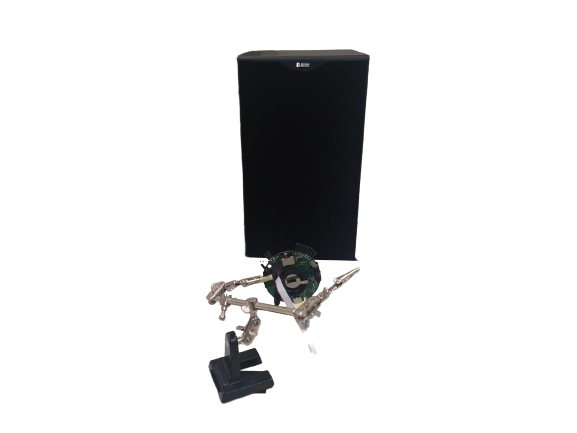
\includegraphics[width=\linewidth]{MEMS_Hinten-removebg} \caption*{(a) MEMS hinten} 
			\end{minipage} 
			\hfill 
			\begin{minipage}
				{0.45\textwidth} 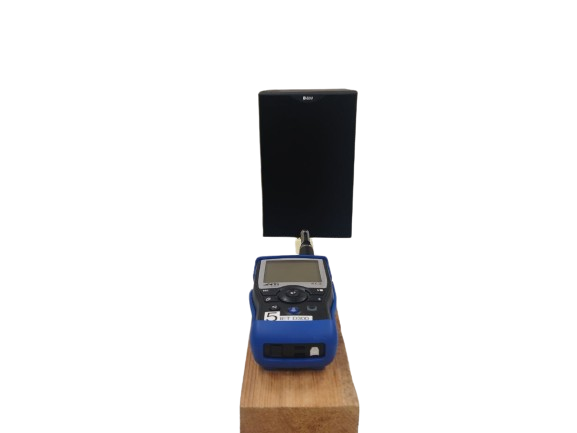
\includegraphics[width=\linewidth]{NTI_Hinten-removebg} \caption*{(b) NTI hinten} 
			\end{minipage} 
			\ 
			\begin{minipage}
				{0.45\textwidth} 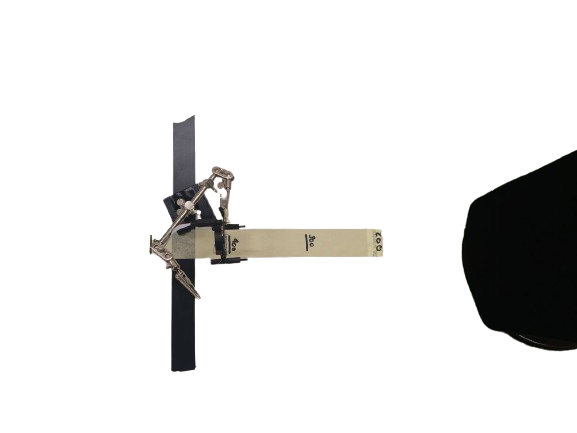
\includegraphics[width=\linewidth]{MEMS_Top-removebg} \caption*{(c) MEMS Vogelperspektive} 
			\end{minipage} 
			\hfill 
			\begin{minipage}
				{0.45\textwidth} 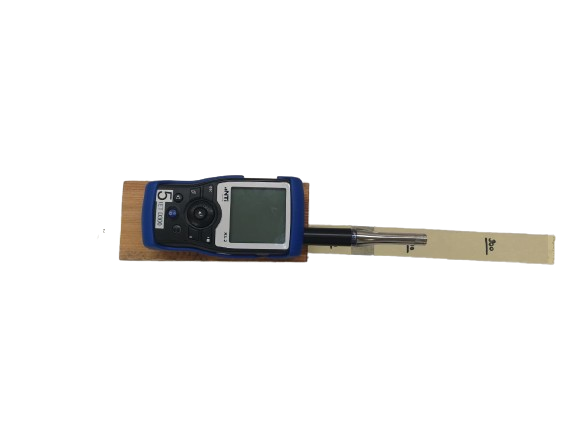
\includegraphics[width=\linewidth]{NTI_Top-removebg} \caption*{(d) NTI Vogelperspektive} 
			\end{minipage}
			\caption[]{Messaufbau Frequenzgang} \label{fig:messaufbau_frequenzgang} 
		\end{figure}
		\begin{figure}[H] 
			\centering 
			\begin{minipage}
				{0.45\textwidth} 		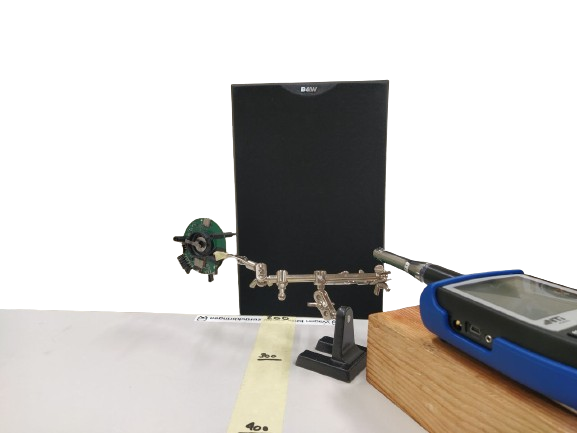
\includegraphics[width=\linewidth]{Beide_Hinten-removebg} \caption*{(a) Messobjekt hinten} 
			\end{minipage} 
			\hfill 
			\begin{minipage}
				{0.45\textwidth} 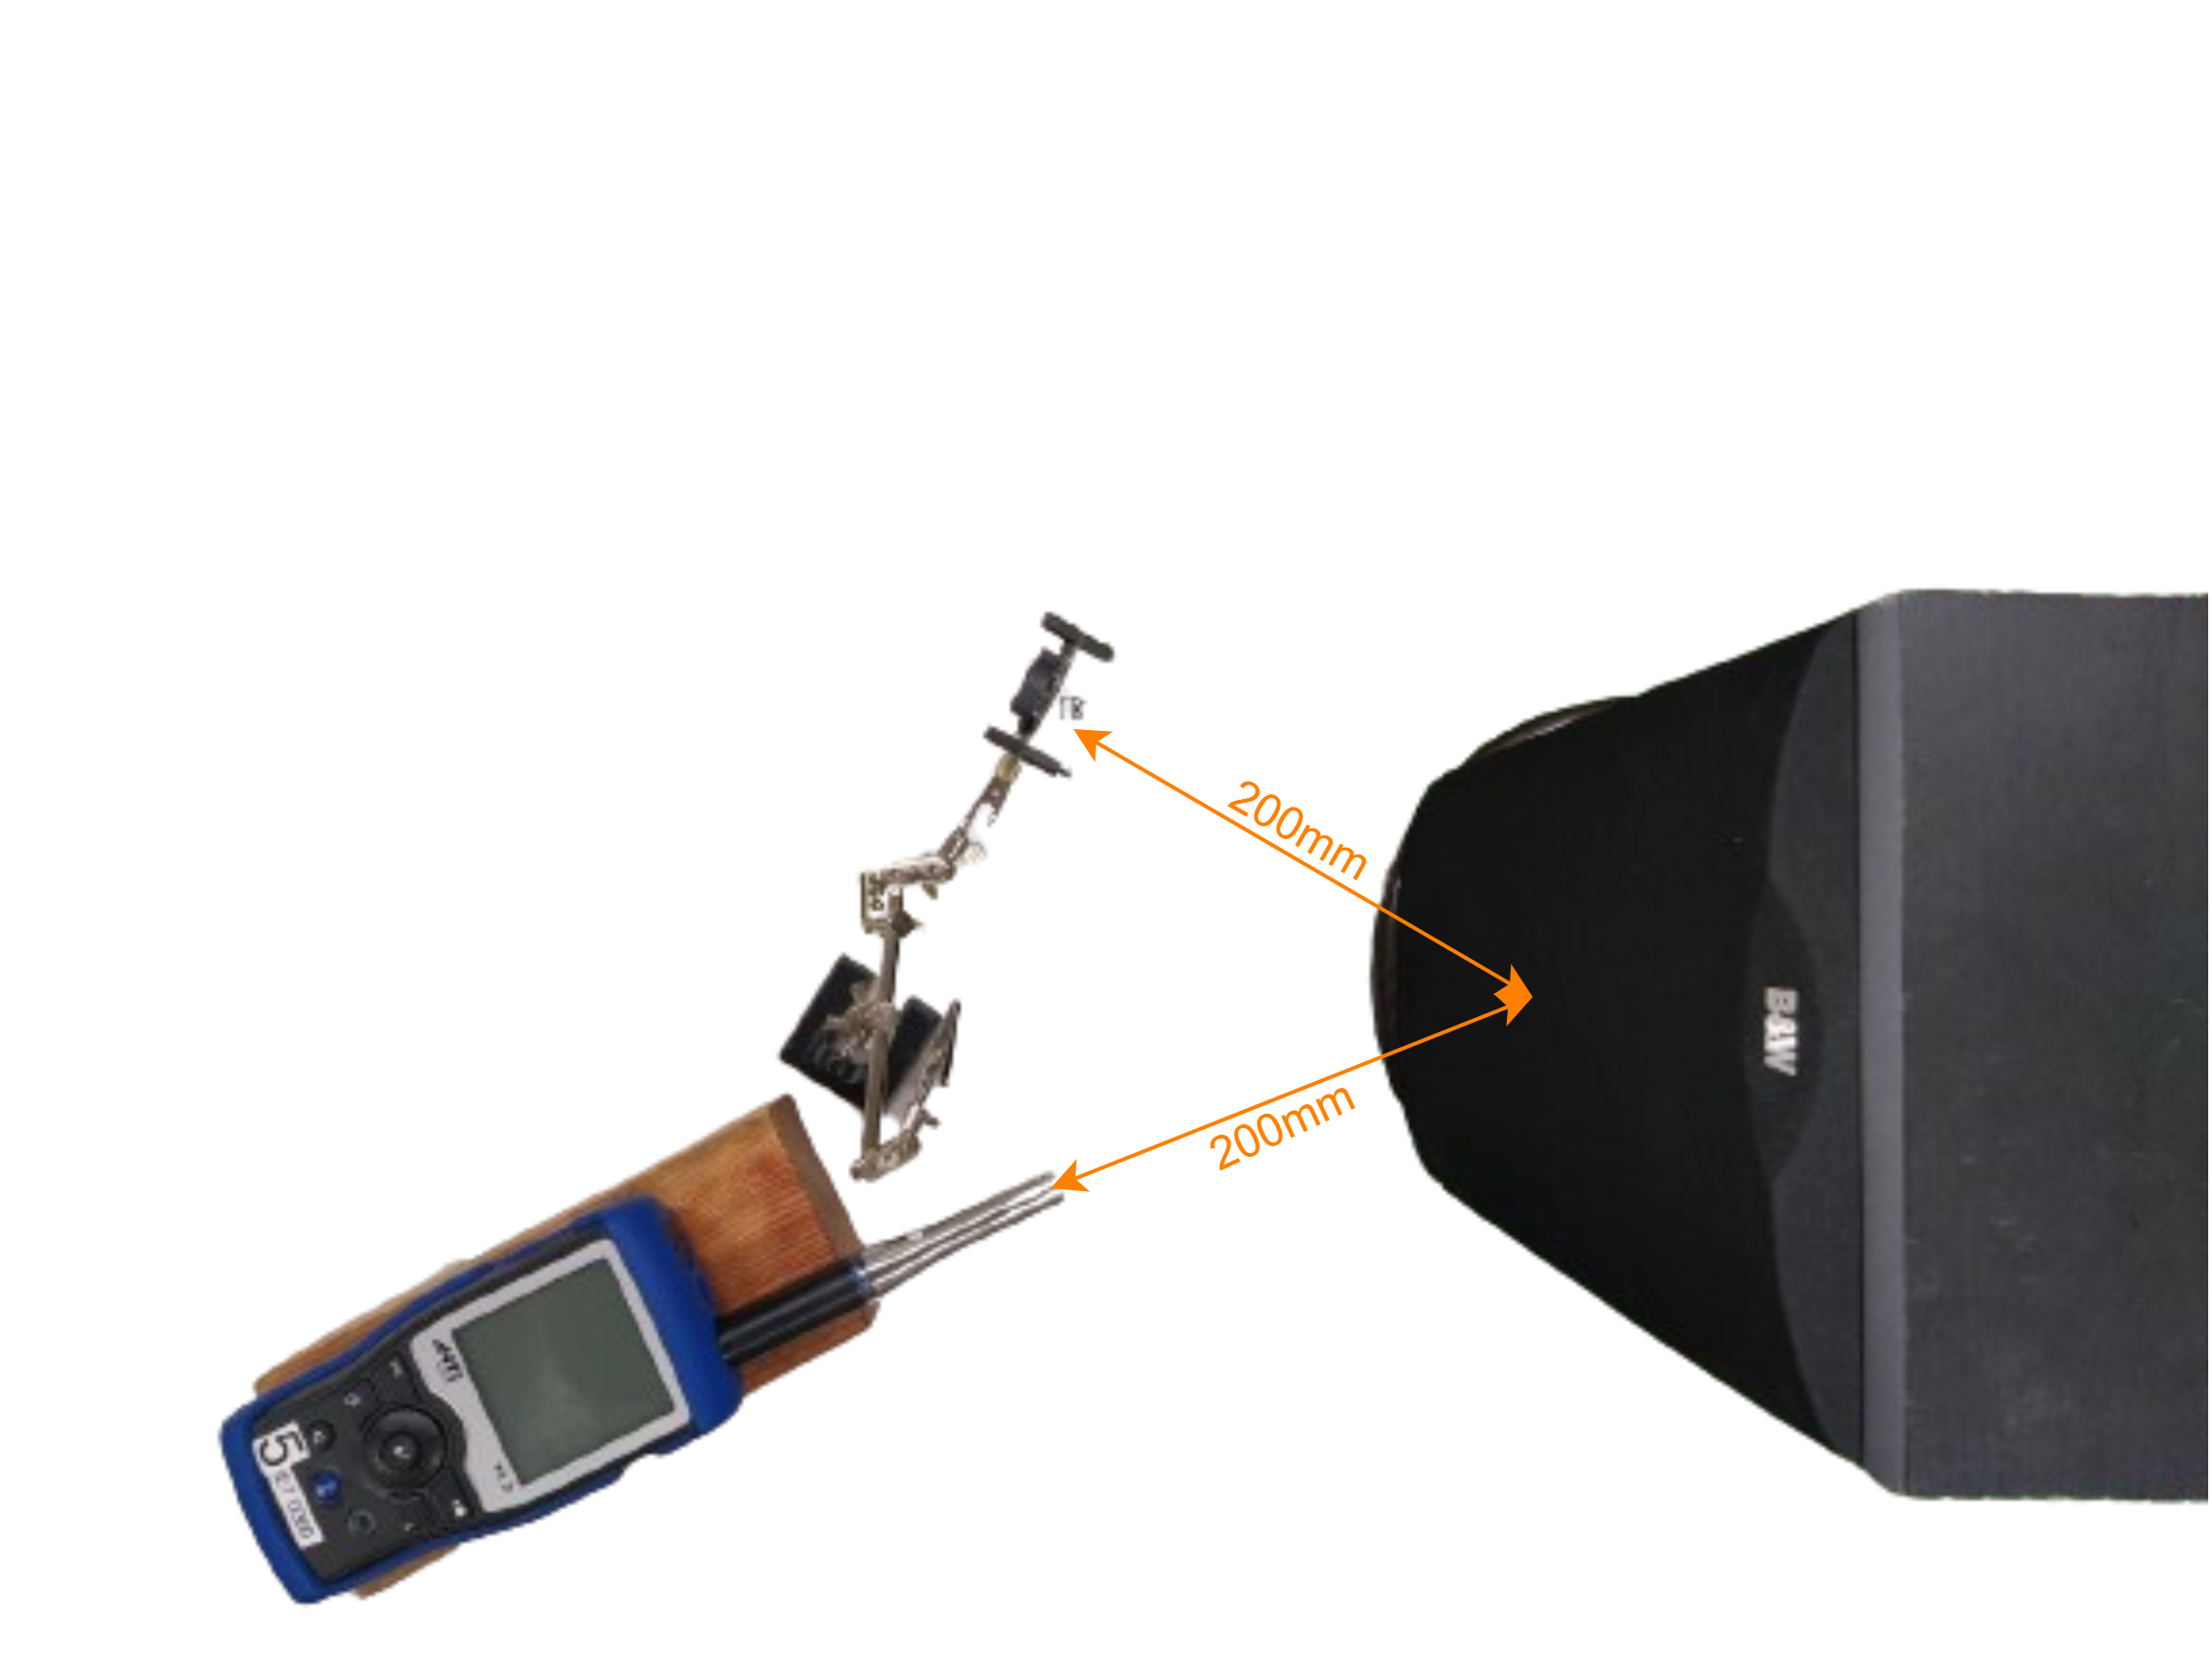
\includegraphics[width=\linewidth]{Beide_Top-removebg} \caption*{(b) Messobjekt Vogelperspektive} 
			\end{minipage} 
			\vfill
			\begin{minipage}
				{1\textwidth} 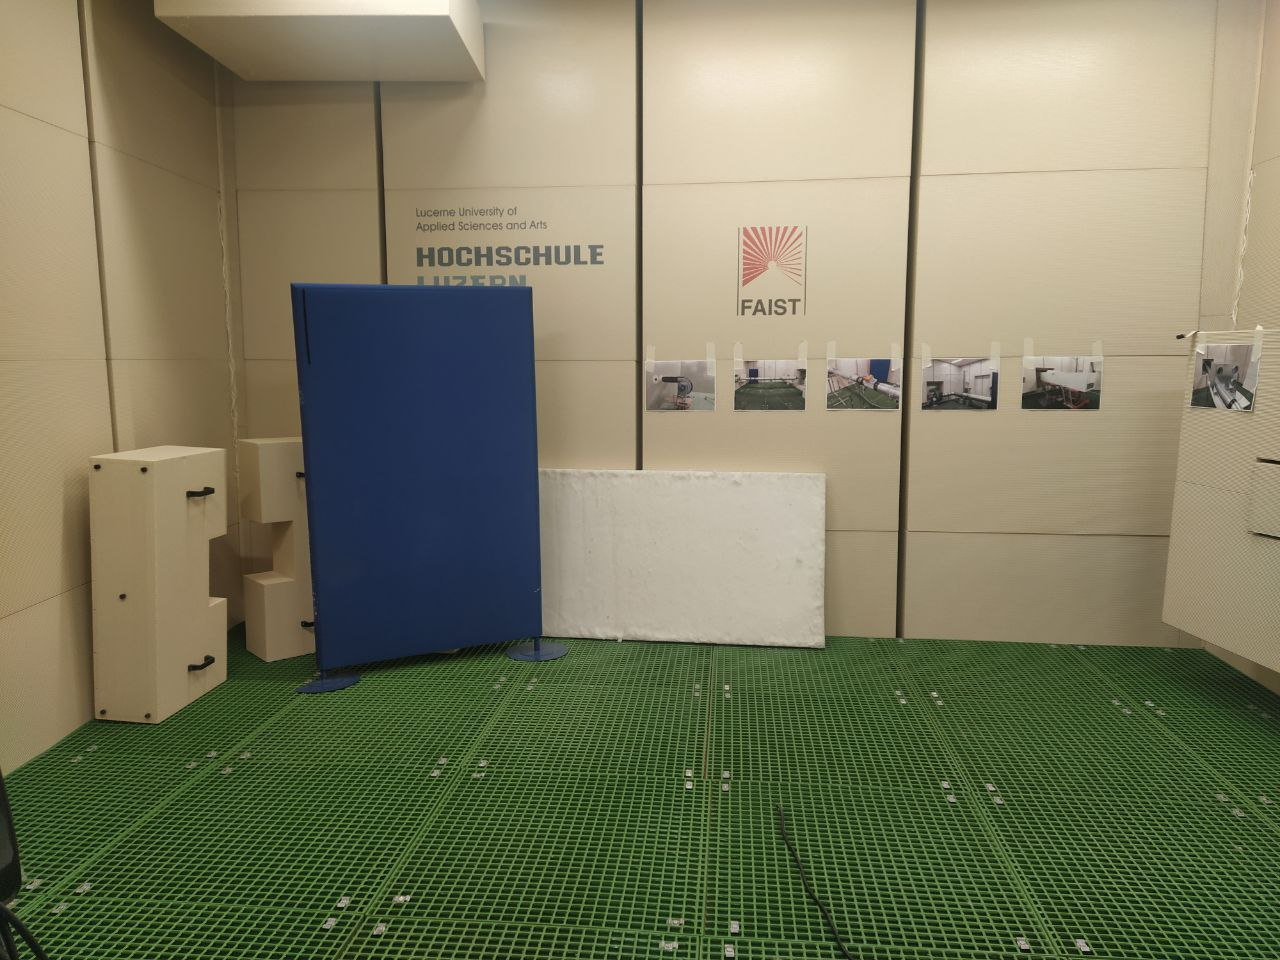
\includegraphics[width=\linewidth]{Raum_leer} \caption*{(c) Reflexionsarme Messkammer} 
			\end{minipage} 
			\caption[]{Messaufbau SPL} \label{fig:messaufbau_spl} 
		\end{figure}
		
	\newpage
	\subsection*{Kalibrationsmessung} \label{Kalibrationsmessung}
	\begin{figure}[H]
		\centering
		\begin{tikzpicture}
			\begin{axis}[
				width=\textwidth,
				xmode=linear,
				%title={Messung ungewichtet},
				xlabel={Distanz zu Schallquelle [mm]},
				ylabel={Schalldruckpegel [dB]},
				xmin=100, xmax=800,
				ymin=60, ymax=100,
				legend pos=north west,
				ymajorgrids=true,
				grid style=dashed,
				]
				\addplot[
				color=blue,
				mark=solid,
				dashed,
				] table[col sep=semicolon, x=Distanz, y=MEMS] {measurements/Microphone/BAT_Frequenzmessung_Kalibration.csv};
				\addlegendentry{$MEMS$}
				\addplot[
				color=red,
				mark=solid,
				dashed,
				] table[col sep=semicolon, x=Distanz, y=Referenz] {measurements/Microphone/BAT_Frequenzmessung_Kalibration.csv};
				\addlegendentry{$M2211$}
				\addplot[
				color=blue,
				mark=solid,
				] table[col sep=semicolon, x=Distanz, y=MEMS_new] {measurements/Microphone/BAT_Frequenzmessung_Kalibration.csv};
				\addlegendentry{$MEMS_{calib}$}
				\addplot[
				color=red,
				mark=solid,
				] table[col sep=semicolon, x=Distanz, y=Referenz_new] {measurements/Microphone/BAT_Frequenzmessung_Kalibration.csv};
				\addlegendentry{$M2211_{calib}$}
			\end{axis}
		\end{tikzpicture}
		\caption[]{Kalibrationsmessung über die Distanz}
		\label{fig:microphone_plot_kalibration}
	\end{figure}
	\begin{table}[H]
		\centering
		\begin{tabular}{|c|c|c|c|}
			\hline
			\textbf{Distanz [mm]} & \textbf{MEMS} & \textbf{Referenz} & \textbf{Delta} \\ \hline
			100 & 83.7 & 87.1 & 3.4 \\ \hline
			200 & 78 & 82.7 & 4.7 \\ \hline
			300 & 76.3 & 80.6 & 4.3 \\ \hline
			400 & 74.5 & 79.9 & 5.4 \\ \hline
			500 & 73.1 & 78.2 & 5.1 \\ \hline
			600 & 70.8 & 77.5 & 6.7 \\ \hline
			700 & 70.7 & 77.1 & 6.4 \\ \hline
			800 & 69.1 & 75.5 & 6.4 \\ \hline
		\end{tabular}
	\end{table}
	
	\newpage
	\subsection*{Grundrauschen $\vert$ Rauschboden} \label{Grundrauschen}
	Eine Vielzahl von Störquellen können die Signalqualität, trotz digitaler Signalverarbeitung, beeinträchtigen. Im Anschluss werden folgende Quellen untersucht:
	\begin{itemize}
		\item Clock-Stabilität $\vert$ Clock-Drift \\
		Wie Konstant ist der Clock, welcher vom Mikrocontroller generiert wird?
		\item Spannungsversorgung \\
		Hat die Speisung via USB einen Einfluss auf den Rauschboden?
		\item Start-Zeit des Mikrofons \\
		Reichen die 20ms, welche gemäss Datenblatt als Startzeit angegeben sind, um das Mikrofon komplett zu starten?
	\end{itemize}
	\paragraph{Clock-Stabilität}\mbox{}\\
	Abbildungen \ref{fig:PDM_CLK_Jitter_Logic-Analyzer} und \ref{fig:PDM_CLK_Jitter_Oszilloskop} zeigen, dass der Clock im Mittel die gewünschte Taktrate von 3.072MHz erreicht. Gleichzeitig weist der Clock eine maximale Abweichung von 1.7\% auf.
	\begin{figure}[H]
		\centering
		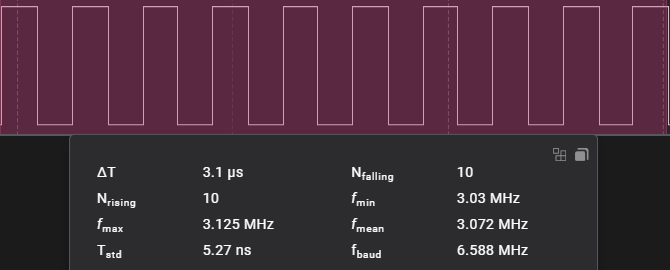
\includegraphics[width=1\linewidth]{measurements/Timings/PDM_CLK_Jitter_Logic-Analyzer}
		\caption[]{Clock-Stabilität gemessen mit Logic Analyzer}
		\label{fig:PDM_CLK_Jitter_Logic-Analyzer}
	\end{figure}
	\begin{figure}[H]
		\centering
		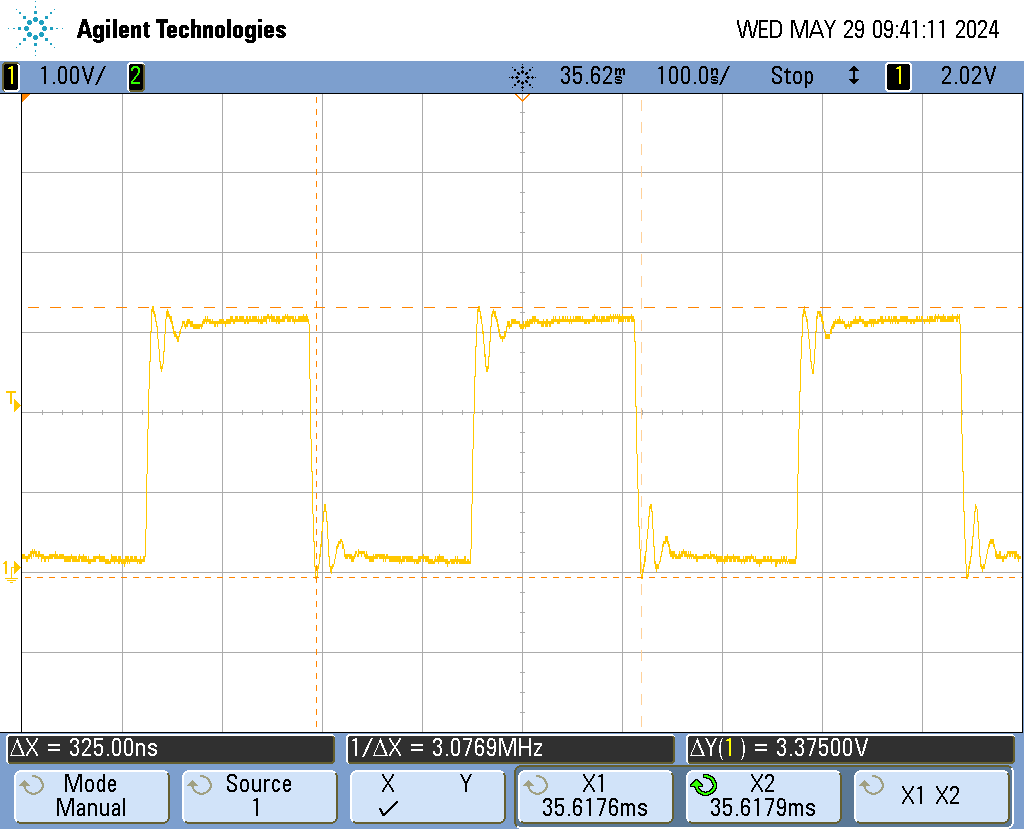
\includegraphics[width=1\linewidth]{measurements/Timings/PDM_CLK_Jitter_Oszilloskop}
		\caption[]{Clock-Stabilität gemessen mit Oszilloskop}
		\label{fig:PDM_CLK_Jitter_Oszilloskop}
	\end{figure} \newpage
	\paragraph{Spannungsversorgung}\mbox{}\\
	Wie Abbildung \ref{fig:stabilitae_rauschen} zeigt, ist das Rauschen zwar von der Spannungsversorgung abhängig, jedoch relativiert sich dieser Einfluss wieder. Wird der gesamt mögliche Messbereich von 24 Bit (16777216 Abstufungen) betrachtet liegen im Mittel 2000 Messpunkte zwischen der Batteriespeisung und der USB-Speisung. Dies entspricht ca. 0.012\% des gesamten Messbereiches.
	$$Distanz \, [\%] = \frac{Mittlerer \, Abstand}{Messbereich}\cdot 100 $$
	\begin{figure}[H]
		\centering
		\begin{tikzpicture}
			\begin{axis}[
				width=\textwidth,
				xmode=linear,
				%title={Messung ungewichtet},
				xlabel={Sample},
				ylabel={PCM-Wert [24-bit Auflösung]},
				xmin=0, xmax=2048,
				ymin=190000, ymax=210000,
				legend pos=north west,
				ymajorgrids=true,
				grid style=dashed,
				]
				\addplot[
				color=green,
				mark=solid,
				] table[col sep=semicolon, x=Sample, y=usb] {measurements/Microphone/BAT_Rauschboden_Speisung.csv};
				\addlegendentry{USB}
				\addplot[
				color=red,
				mark=solid,
				] table[col sep=semicolon, x=Sample, y=batterie] {measurements/Microphone/BAT_Rauschboden_Speisung.csv};
				\addlegendentry{Batterie}
				\addplot[
				color=blue,
				mark=solid,
				] table[col sep=semicolon, x=Sample, y=usb_batterie] {measurements/Microphone/BAT_Rauschboden_Speisung.csv};
				\addlegendentry{USB und Batterie}
			\end{axis}
		\end{tikzpicture}
		\caption[]{Einfluss von Spannungsquellen auf das Mikrofonrauschen}
		\label{fig:stabilitae_rauschen}
	\end{figure} \newpage
	\paragraph{Start-Zeit}\mbox{}\\
	Abbildung \ref{fig:startzeit-mikrofon} zeigt deutlich, dass das Mikrofon-Grundrauschen verbessert wird, sofern das Mikrofon jeweils nicht nach jeder Messung in den Energiesparmodus versetzt wird. So konnte ein Rauschboden von bis zu 37dB gemessen werden, welcher demjenigen aus dem Datenblatt (\cite{noauthor_httpsinvensensetdkcomwp-contentuploads202007ds-000157-ics-41351-v14pdf_nodate}) sehr nahe kommt. Bei den Messungen im freilaufenden Modus variierte der Rauschboden jedoch um jeweils bis zu 14dB.
	\begin{figure}[H]
		\centering
		\begin{tikzpicture}
			\begin{axis}[
				width=0.95\textwidth,
				xmode=linear,
				%title={Messung ungewichtet},
				xlabel={Sample},
				ylabel={PCM-Wert [24-bit Auflösung]},
				xmin=0, xmax=2048,
				ymin=-5000, ymax=5000,
				legend pos=north west,
				ymajorgrids=true,
				grid style=dashed,
				]
				\addplot[
				color=blue,
				mark=solid,
				] table[col sep=semicolon, x=Sample, y=20ms] {measurements/Microphone/BAT_Rauschboden_Startup.csv};
				\addlegendentry{20ms}
				\addplot[
				color=red,
				mark=solid,
				] table[col sep=semicolon, x=Sample, y=freilaufend] {measurements/Microphone/BAT_Rauschboden_Startup.csv};
				\addlegendentry{Freilaufend}
			\end{axis}
		\end{tikzpicture}
		\caption[]{Einfluss der Startzeit auf das Mikrofonrauschen}
		\label{fig:startzeit-mikrofon}
	\end{figure}
	\paragraph{Fazit}\mbox{}\\
	Die drei Messungen zeigen, dass jede untersuchte Fehlerquelle einen Einfluss auf das SNR hat. Insbesondere das Ein- und Ausschalten des Mikrofons scheint den hohen Rauschboden zu erklären und muss in einer Folgearbeit überarbeitet werden.
	
	\newpage
	\subsection*{PCB-Versionen} \label{PCB-Versionen}
	\begin{figure}[H]
		\centering
		\begin{minipage}{.5\textwidth}
			\centering
			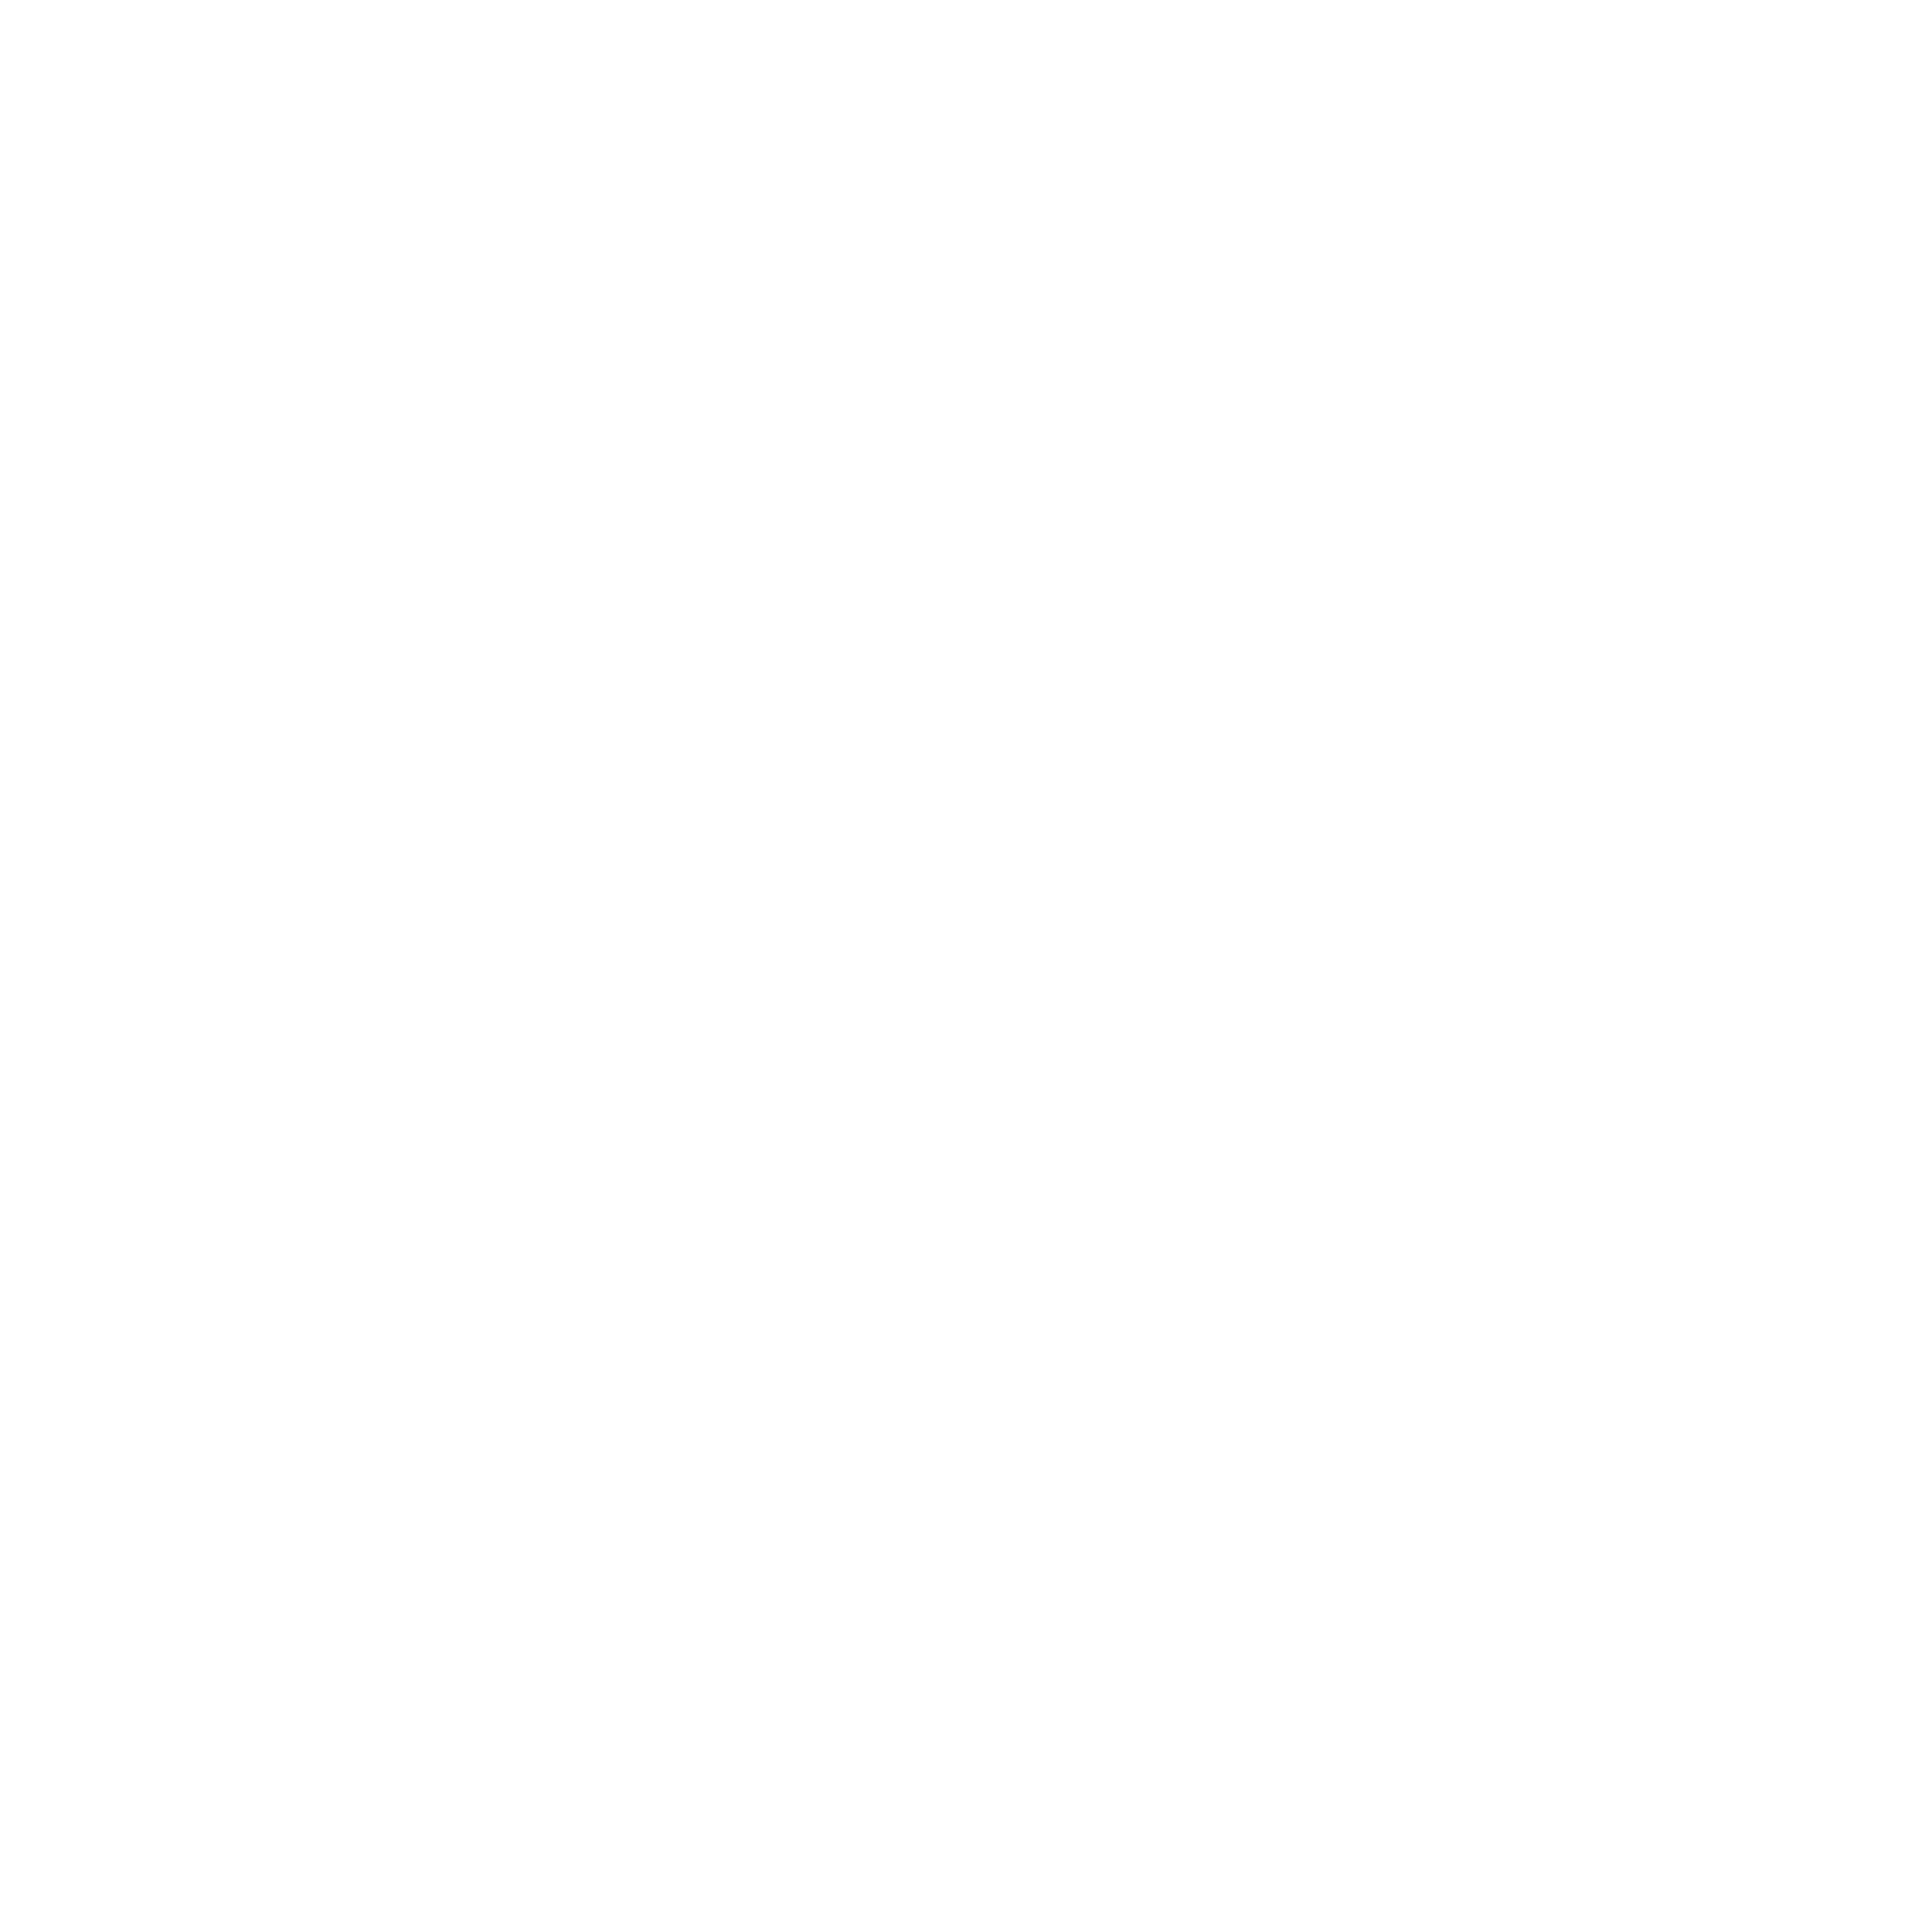
\includegraphics[width=1\linewidth]{images/BAT_PCB_V1-0_top}
			\caption[]{V1-0 Front}
			\label{fig:pcb_V1-0_front}
		\end{minipage}%
		\begin{minipage}{.5\textwidth}
			\centering
			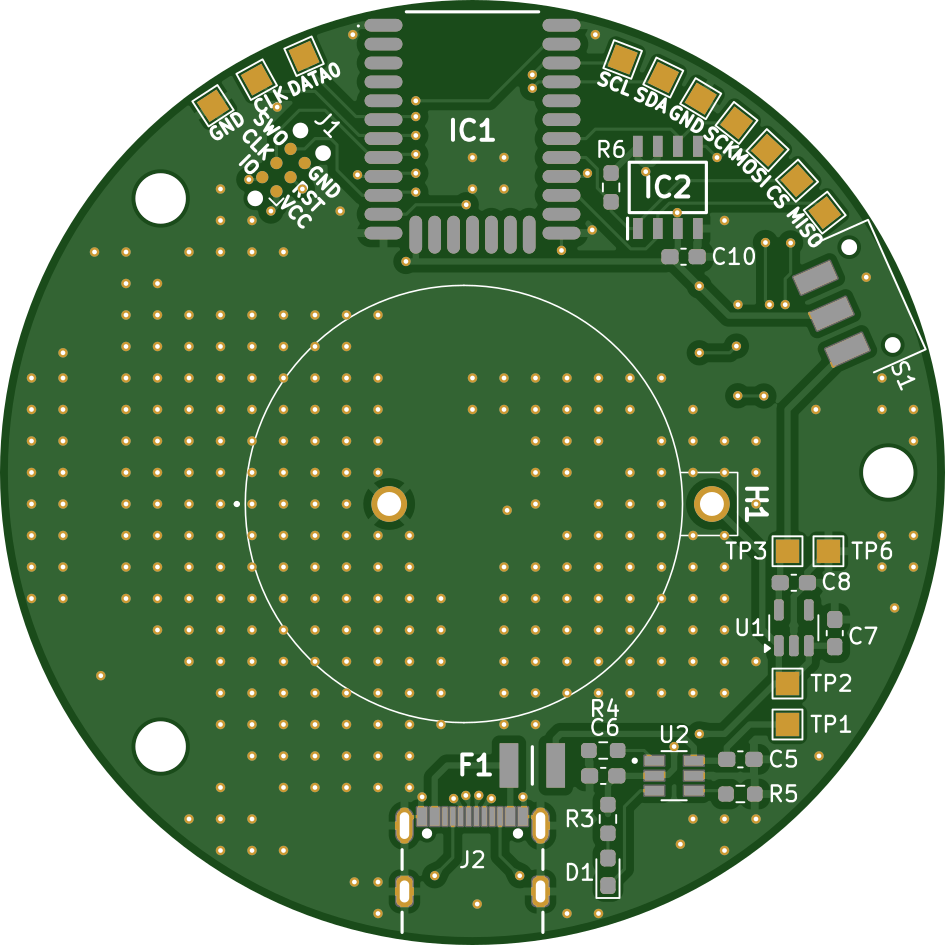
\includegraphics[width=1\linewidth]{images/BAT_PCB_V1-0_bottom}
			\caption[]{V1-0 Back}
			\label{fig:pcb_V1-0_back}
		\end{minipage}
	\end{figure}
	\begin{figure}[H]
		\centering
		\begin{minipage}{.5\textwidth}
			\centering
			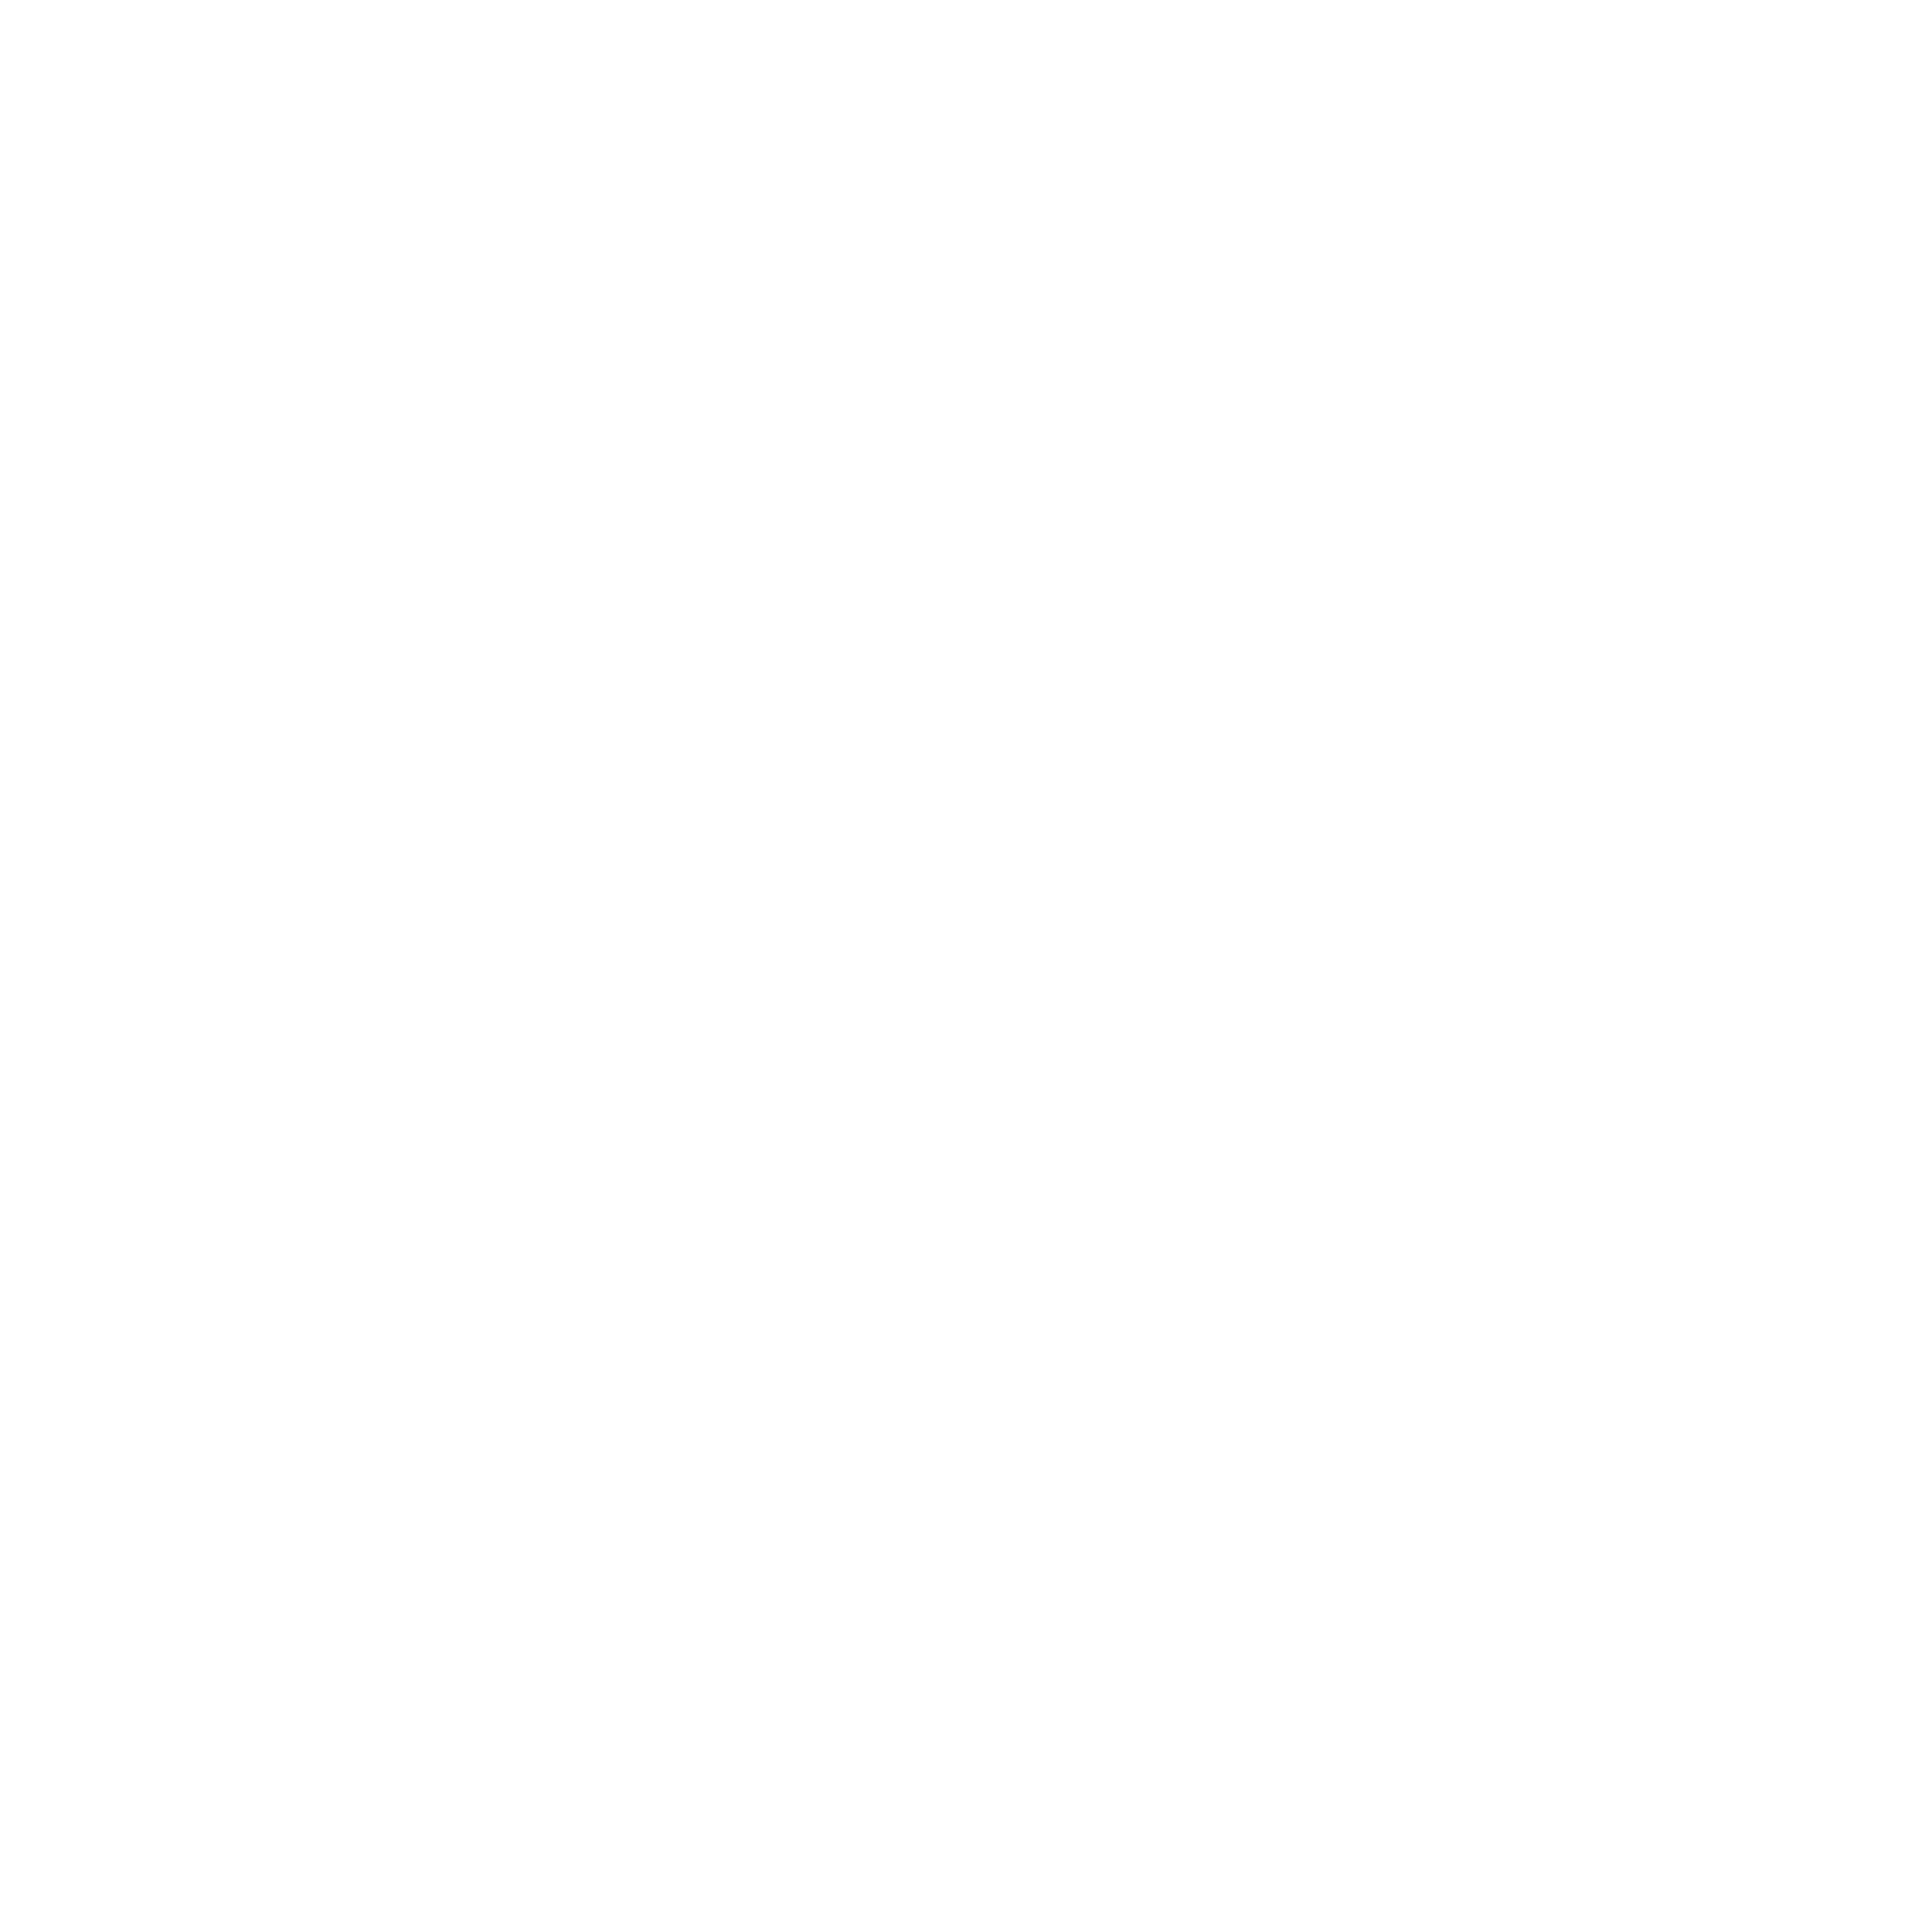
\includegraphics[width=1\linewidth]{images/BAT_PCB_V1-1_top}
			\caption[]{V1-1 Front}
			\label{fig:pcb_V1-1_front}
		\end{minipage}%
		\begin{minipage}{.5\textwidth}
			\centering
			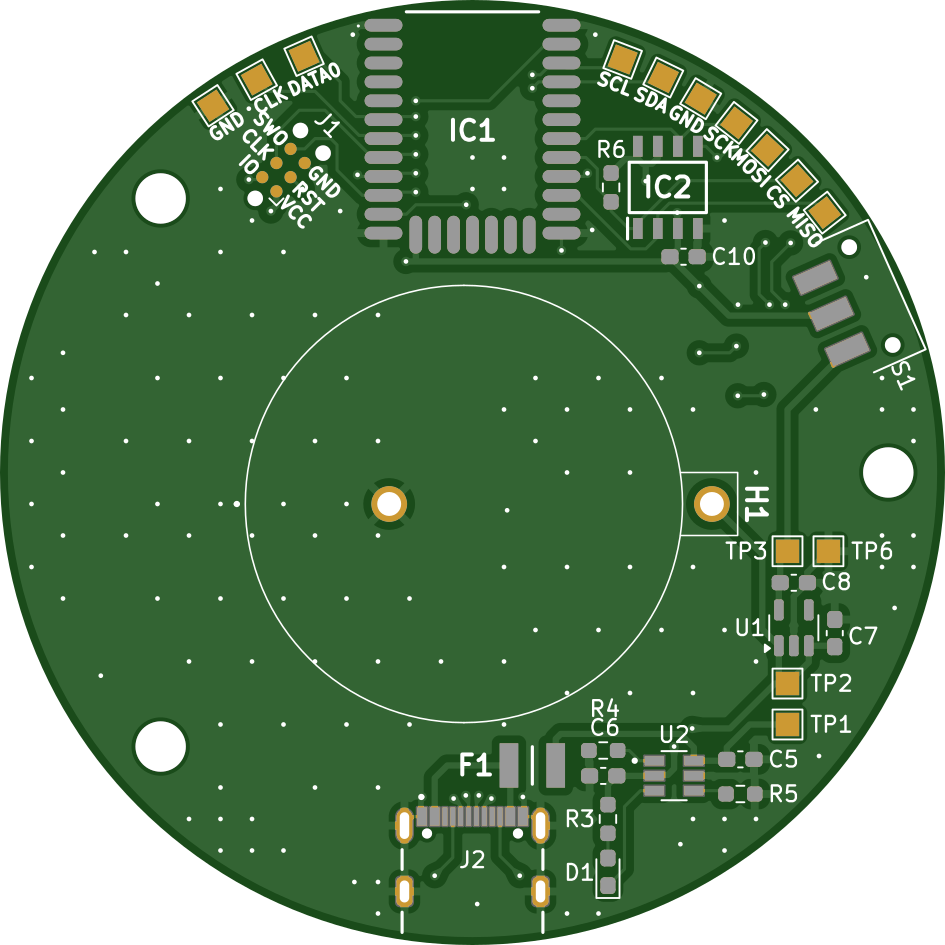
\includegraphics[width=1\linewidth]{images/BAT_PCB_V1-1_bottom}
			\caption[]{V1-1 Back}
			\label{fig:pcb_V1-1_back}
		\end{minipage}
	\end{figure}
	\begin{figure}[H]
		\centering
		\begin{minipage}{.5\textwidth}
			\centering
			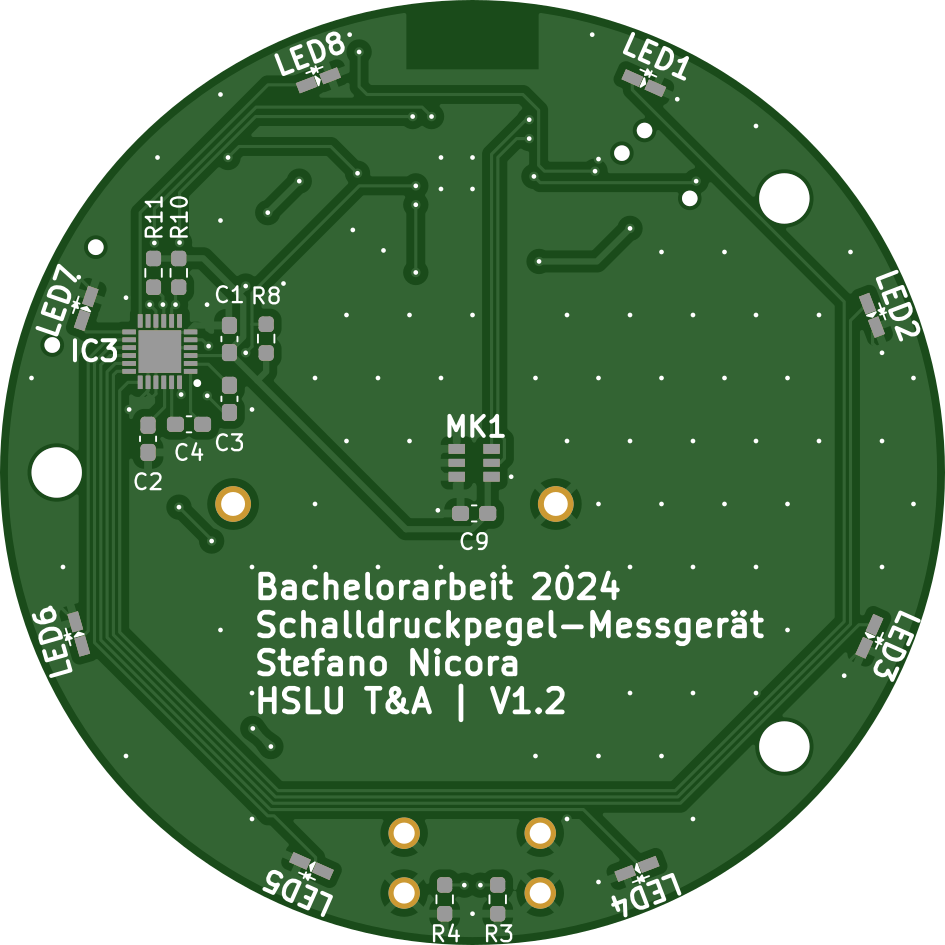
\includegraphics[width=1\linewidth]{images/BAT_PCB_V1-2_top}
			\caption[]{V1-2 Front}
			\label{fig:pcb_V1-2_front}
		\end{minipage}%
		\begin{minipage}{.5\textwidth}
			\centering
			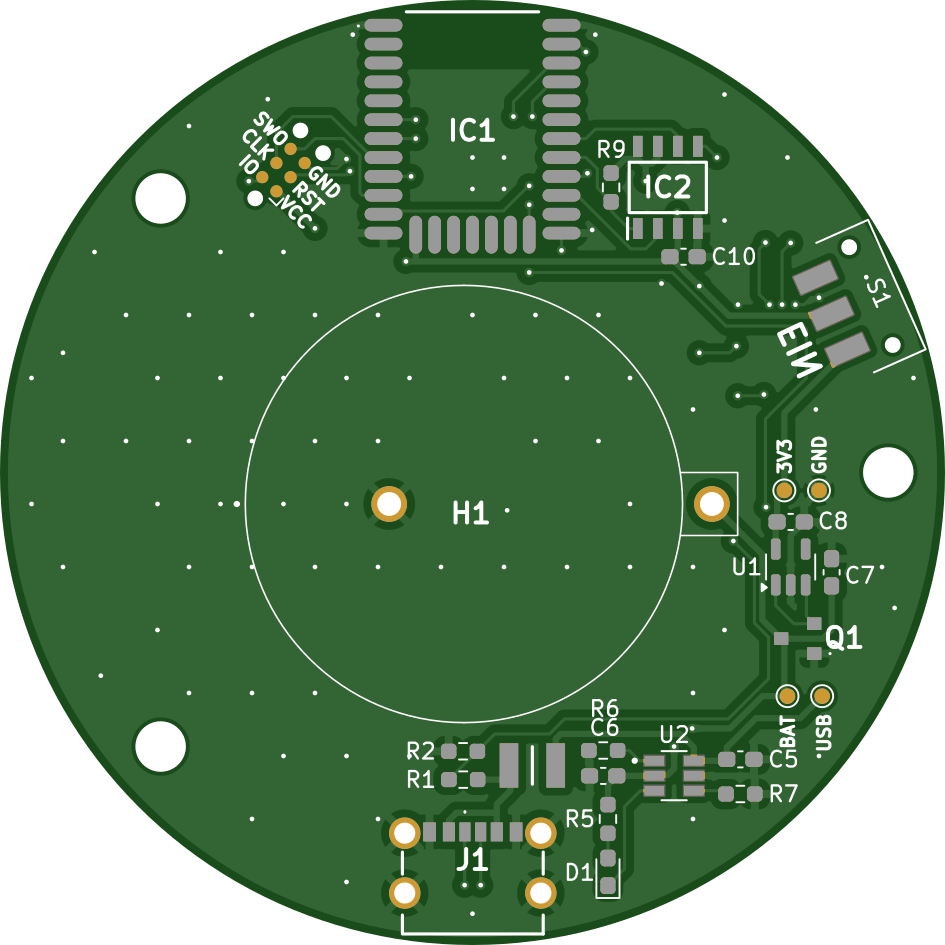
\includegraphics[width=1\linewidth]{images/BAT_PCB_V1-2_bottom}
			\caption[]{V1-2 Back}
			\label{fig:pcb_V1-2_back}
		\end{minipage}
	\end{figure}
	\begin{figure}[H]
		\centering
		\begin{minipage}{.5\textwidth}
			\centering
			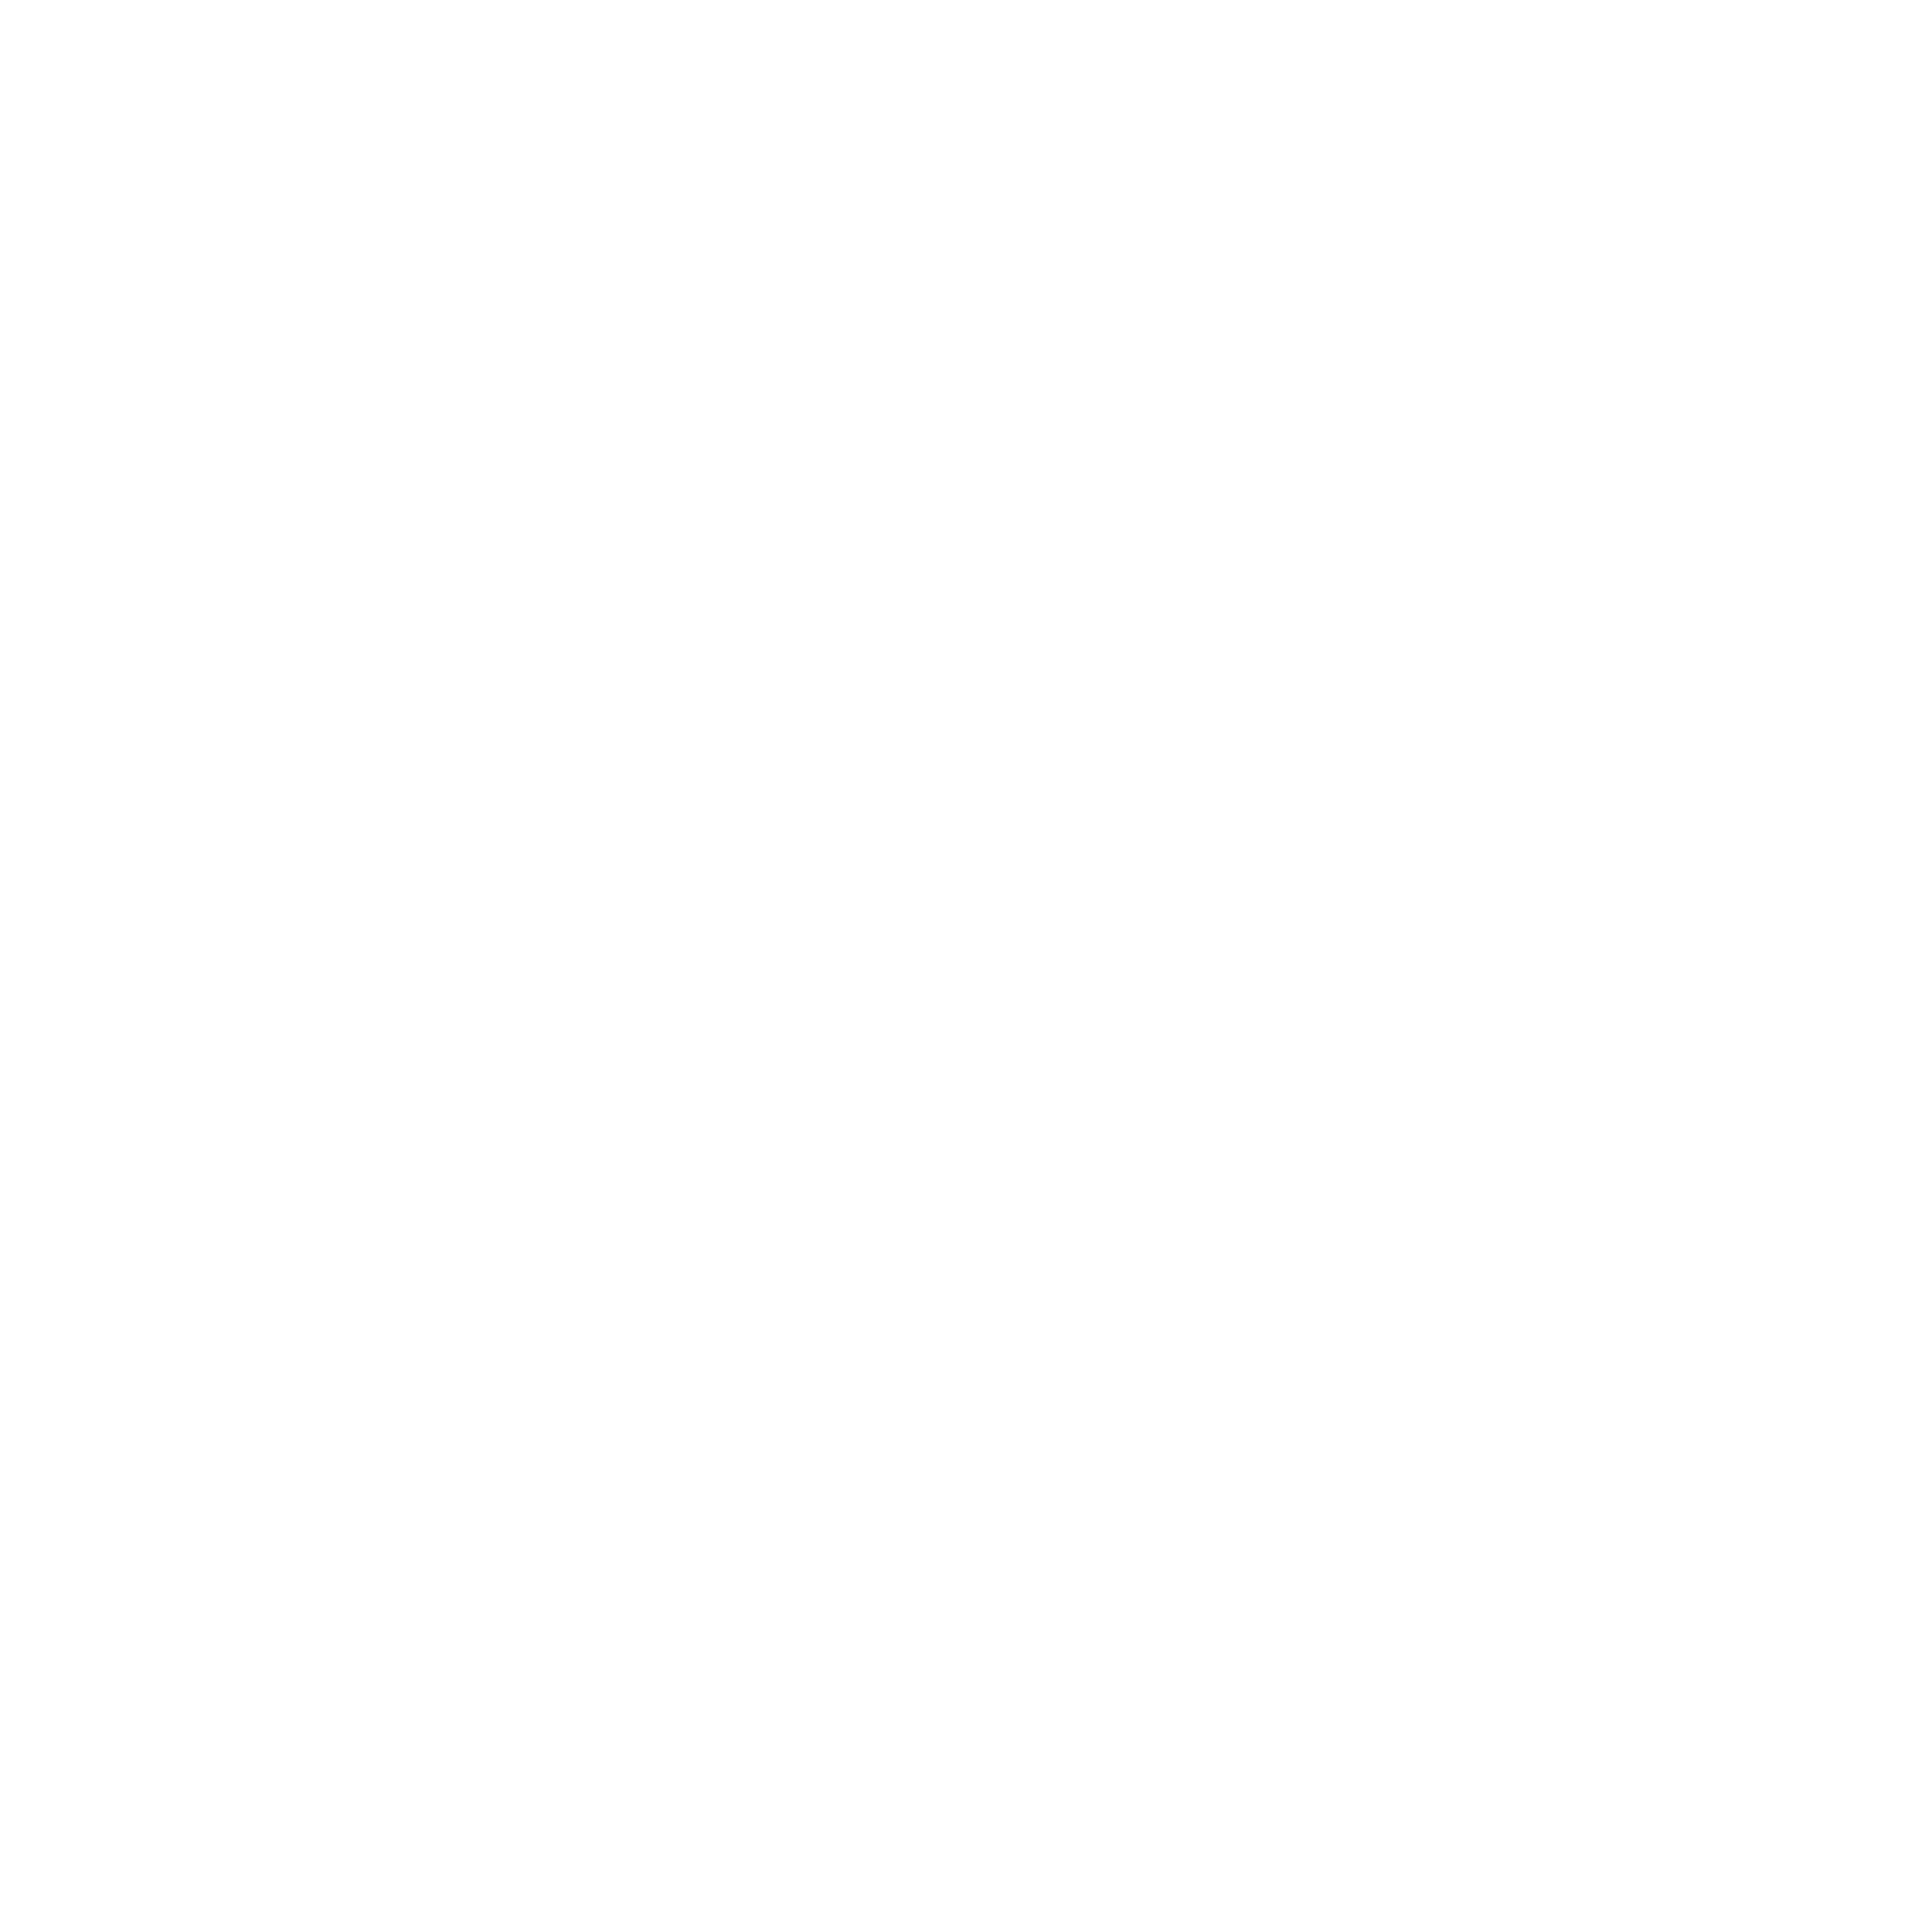
\includegraphics[width=1\linewidth]{images/BAT_PCB_V1-3_top}
			\caption[]{V1-3 Front}
			\label{fig:pcb_V1-3_front}
		\end{minipage}%
		\begin{minipage}{.5\textwidth}
			\centering
			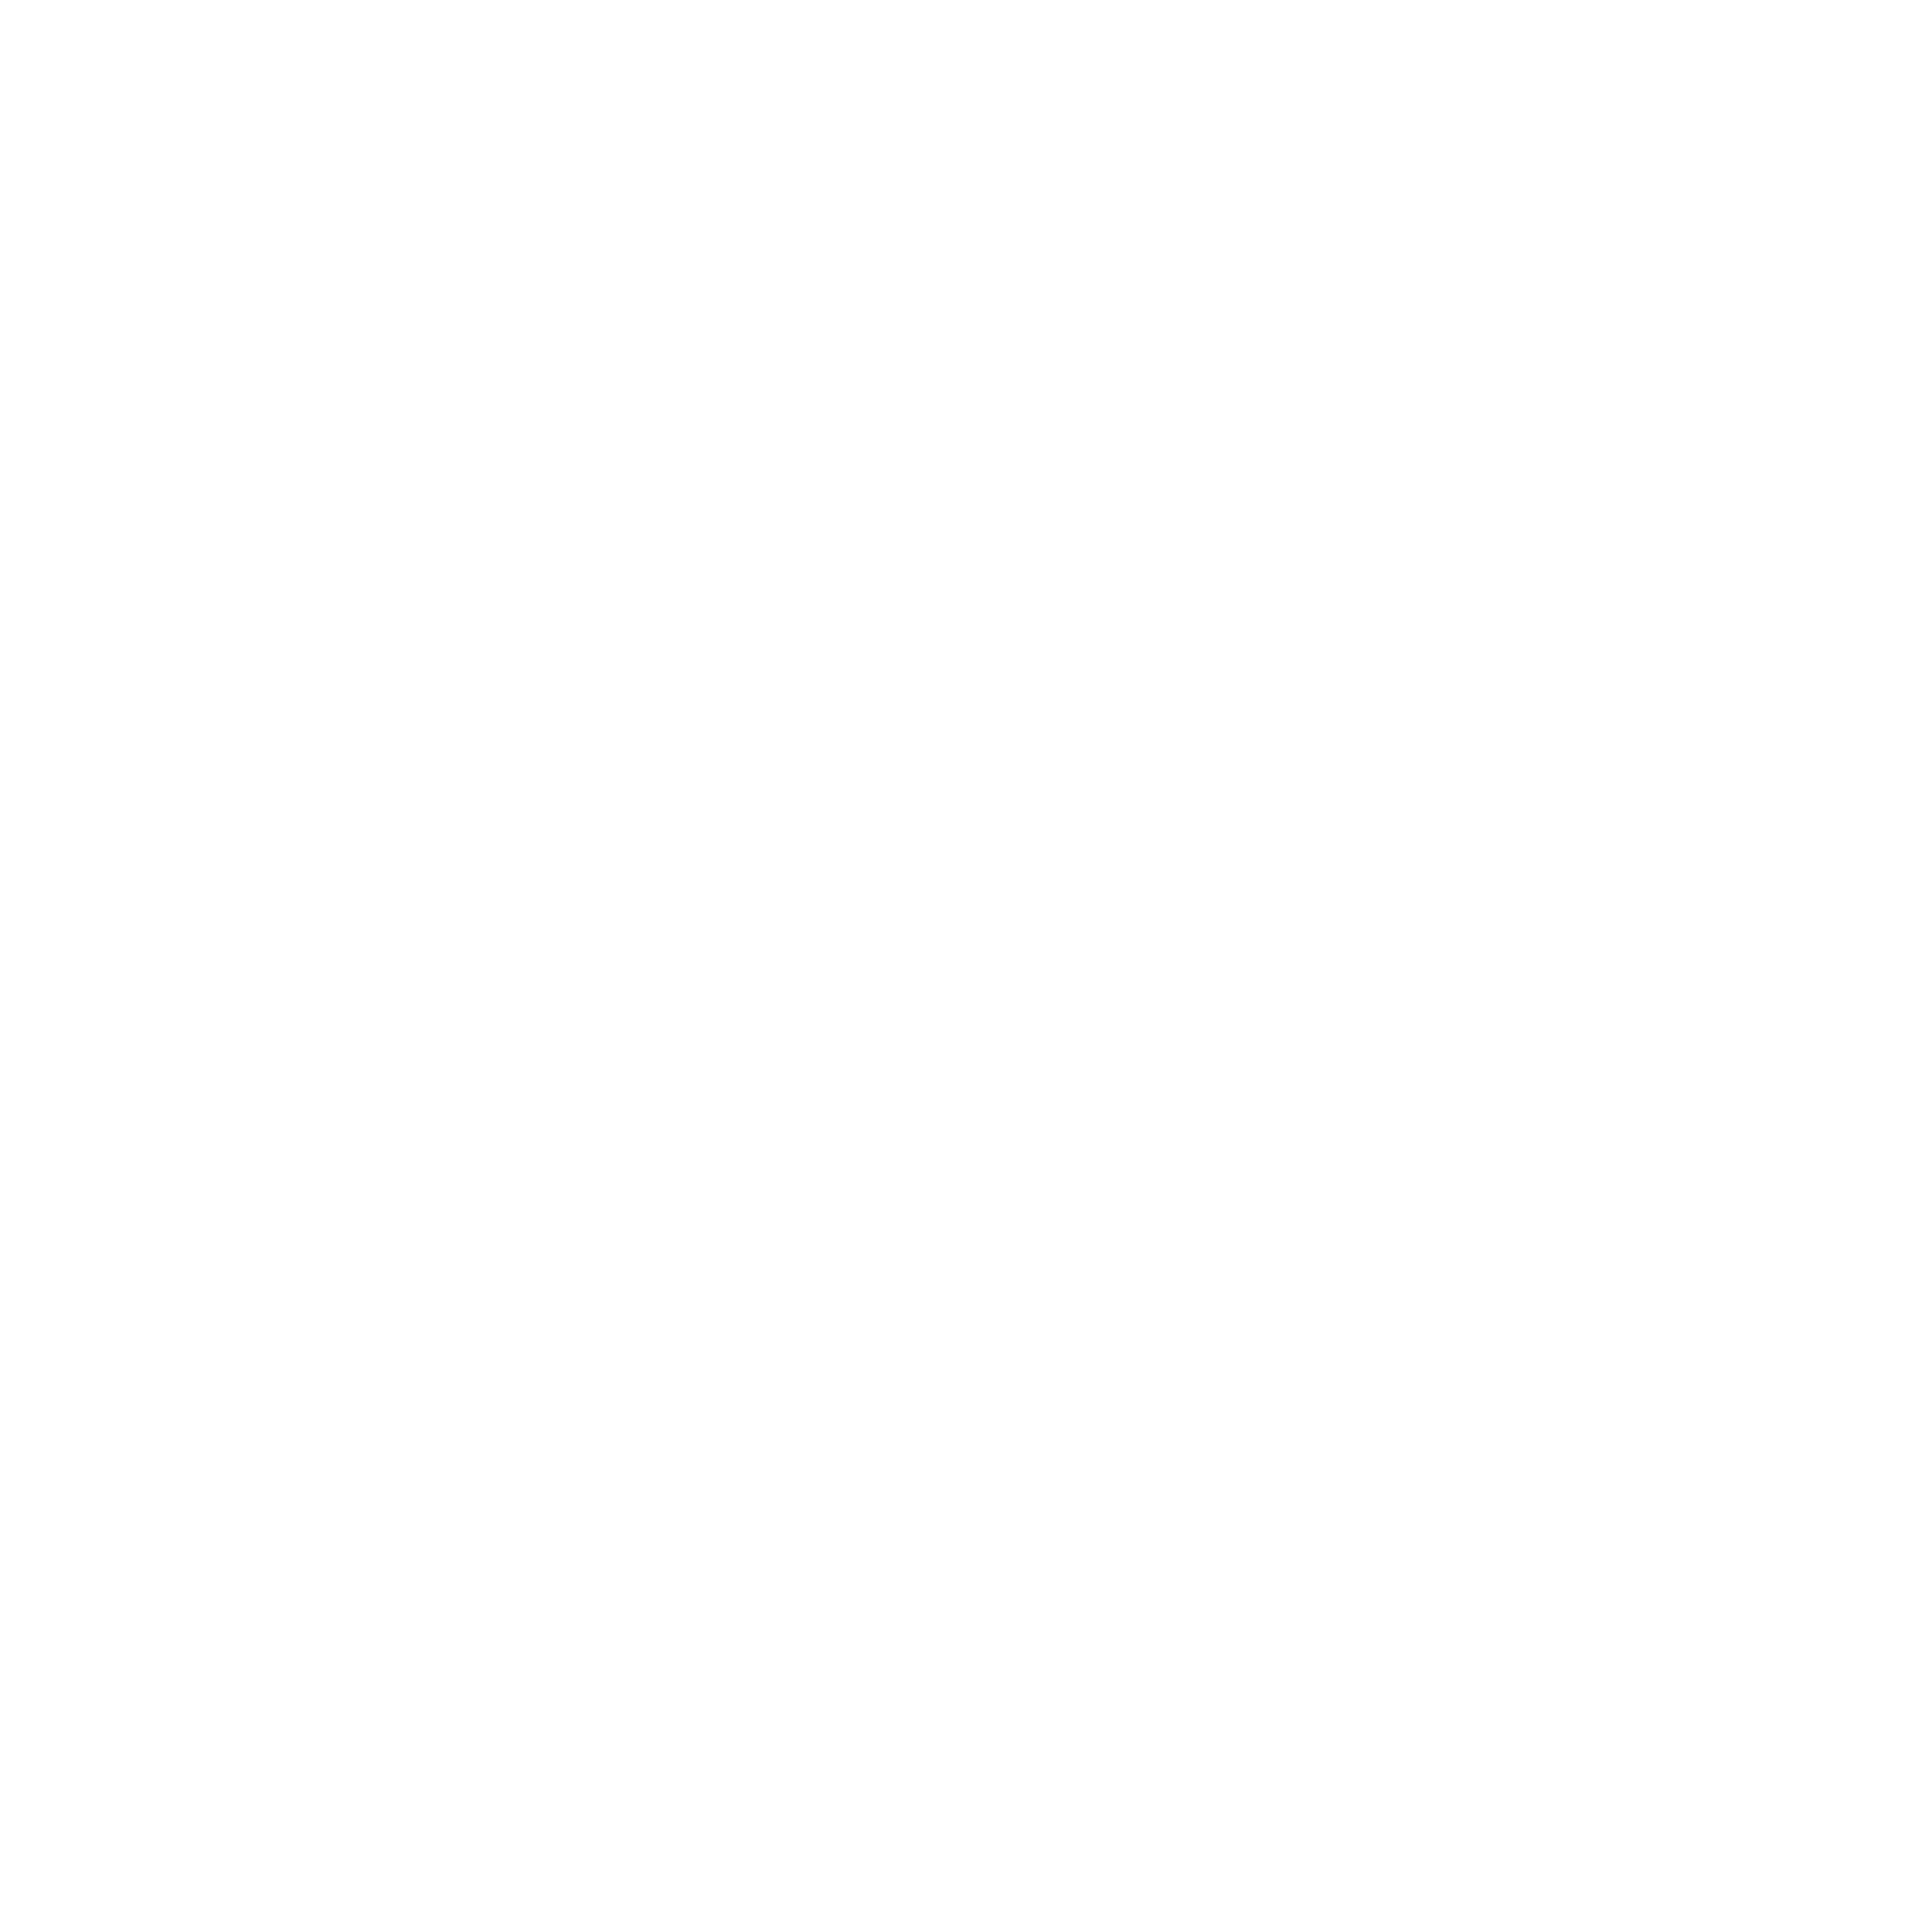
\includegraphics[width=1\linewidth]{images/BAT_PCB_V1-3_bottom}
			\caption[]{V1-3 Back}
			\label{fig:pcb_V1-3_back}
		\end{minipage}
	\end{figure} 
	
	\newpage
	\subsection*{Schema}
	%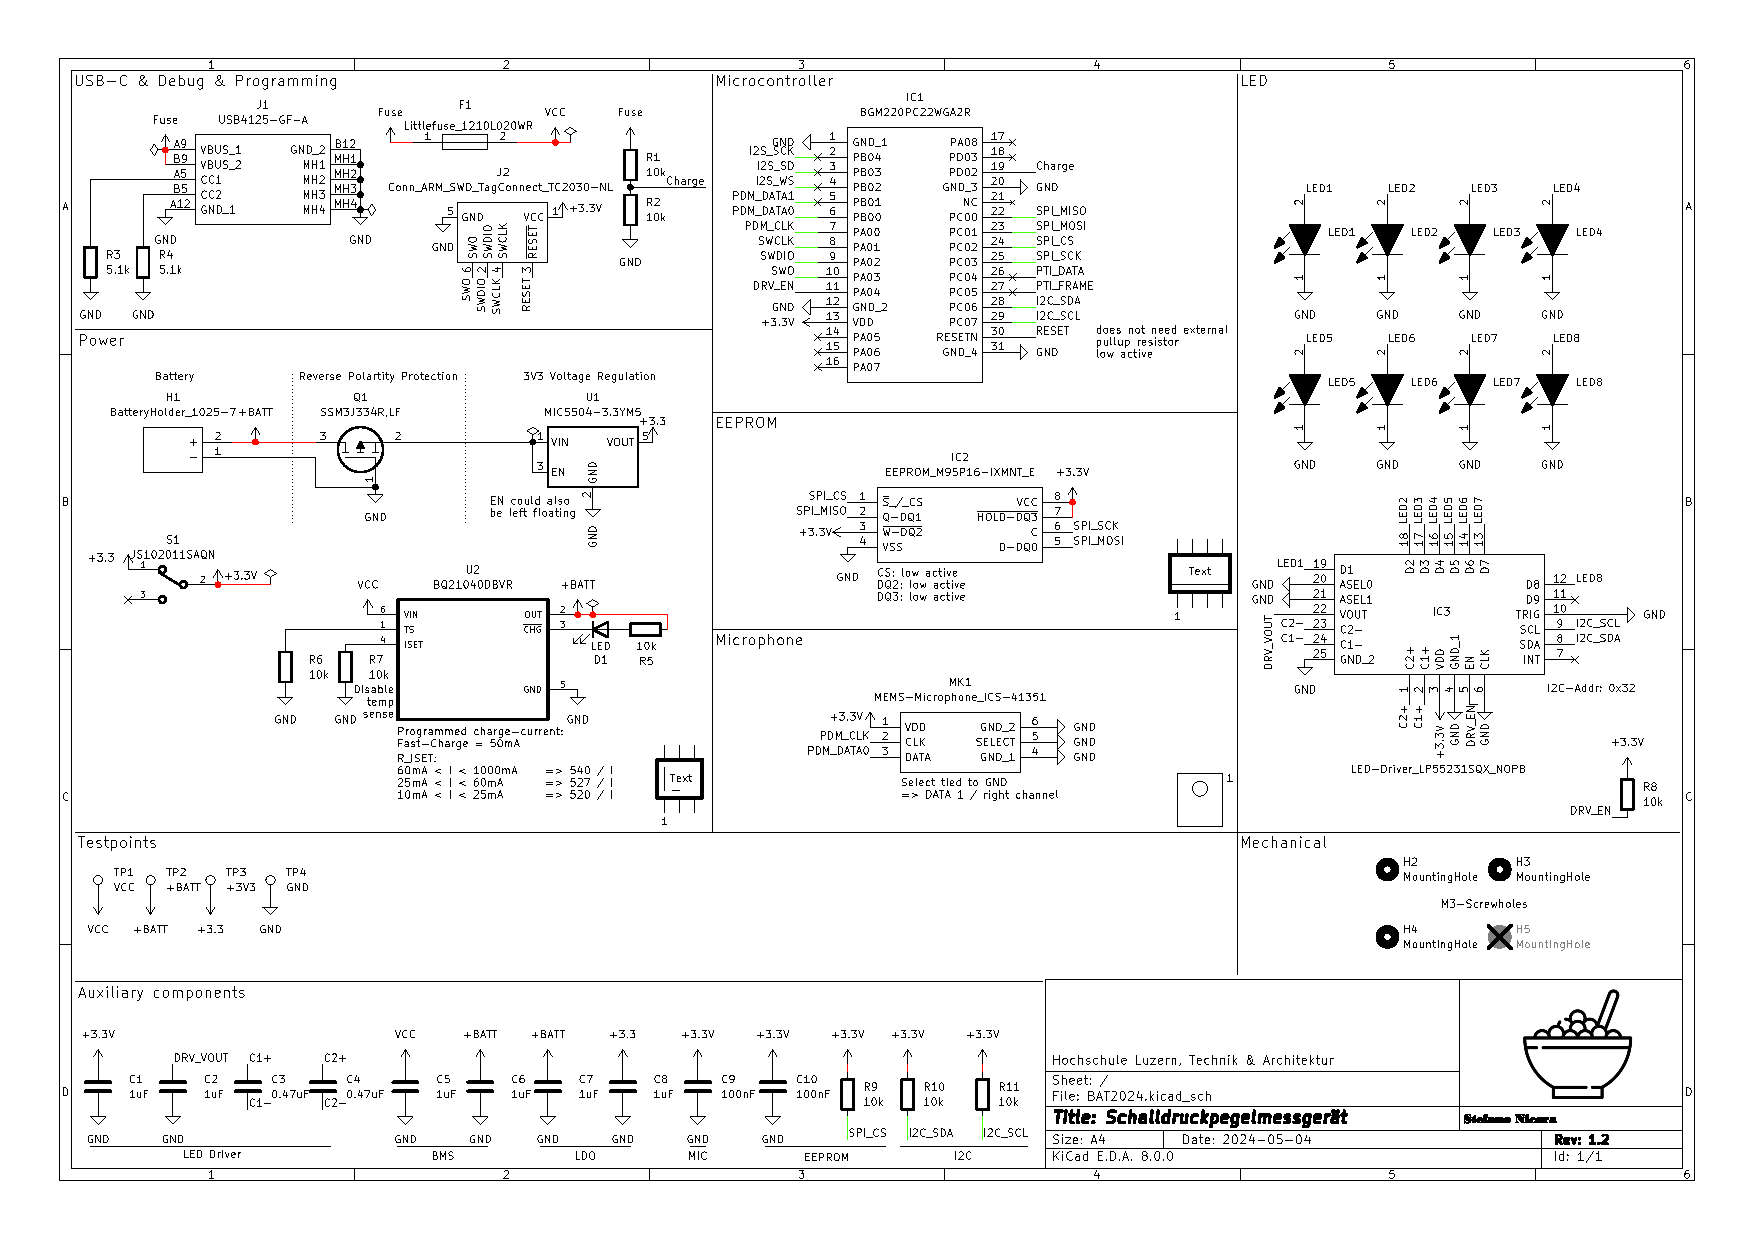
\includepdf[landscape=true, pages={1}]{images/BAT_Schematic_V1-2.pdf}
	\begin{minipage}[b]{\textwidth}
		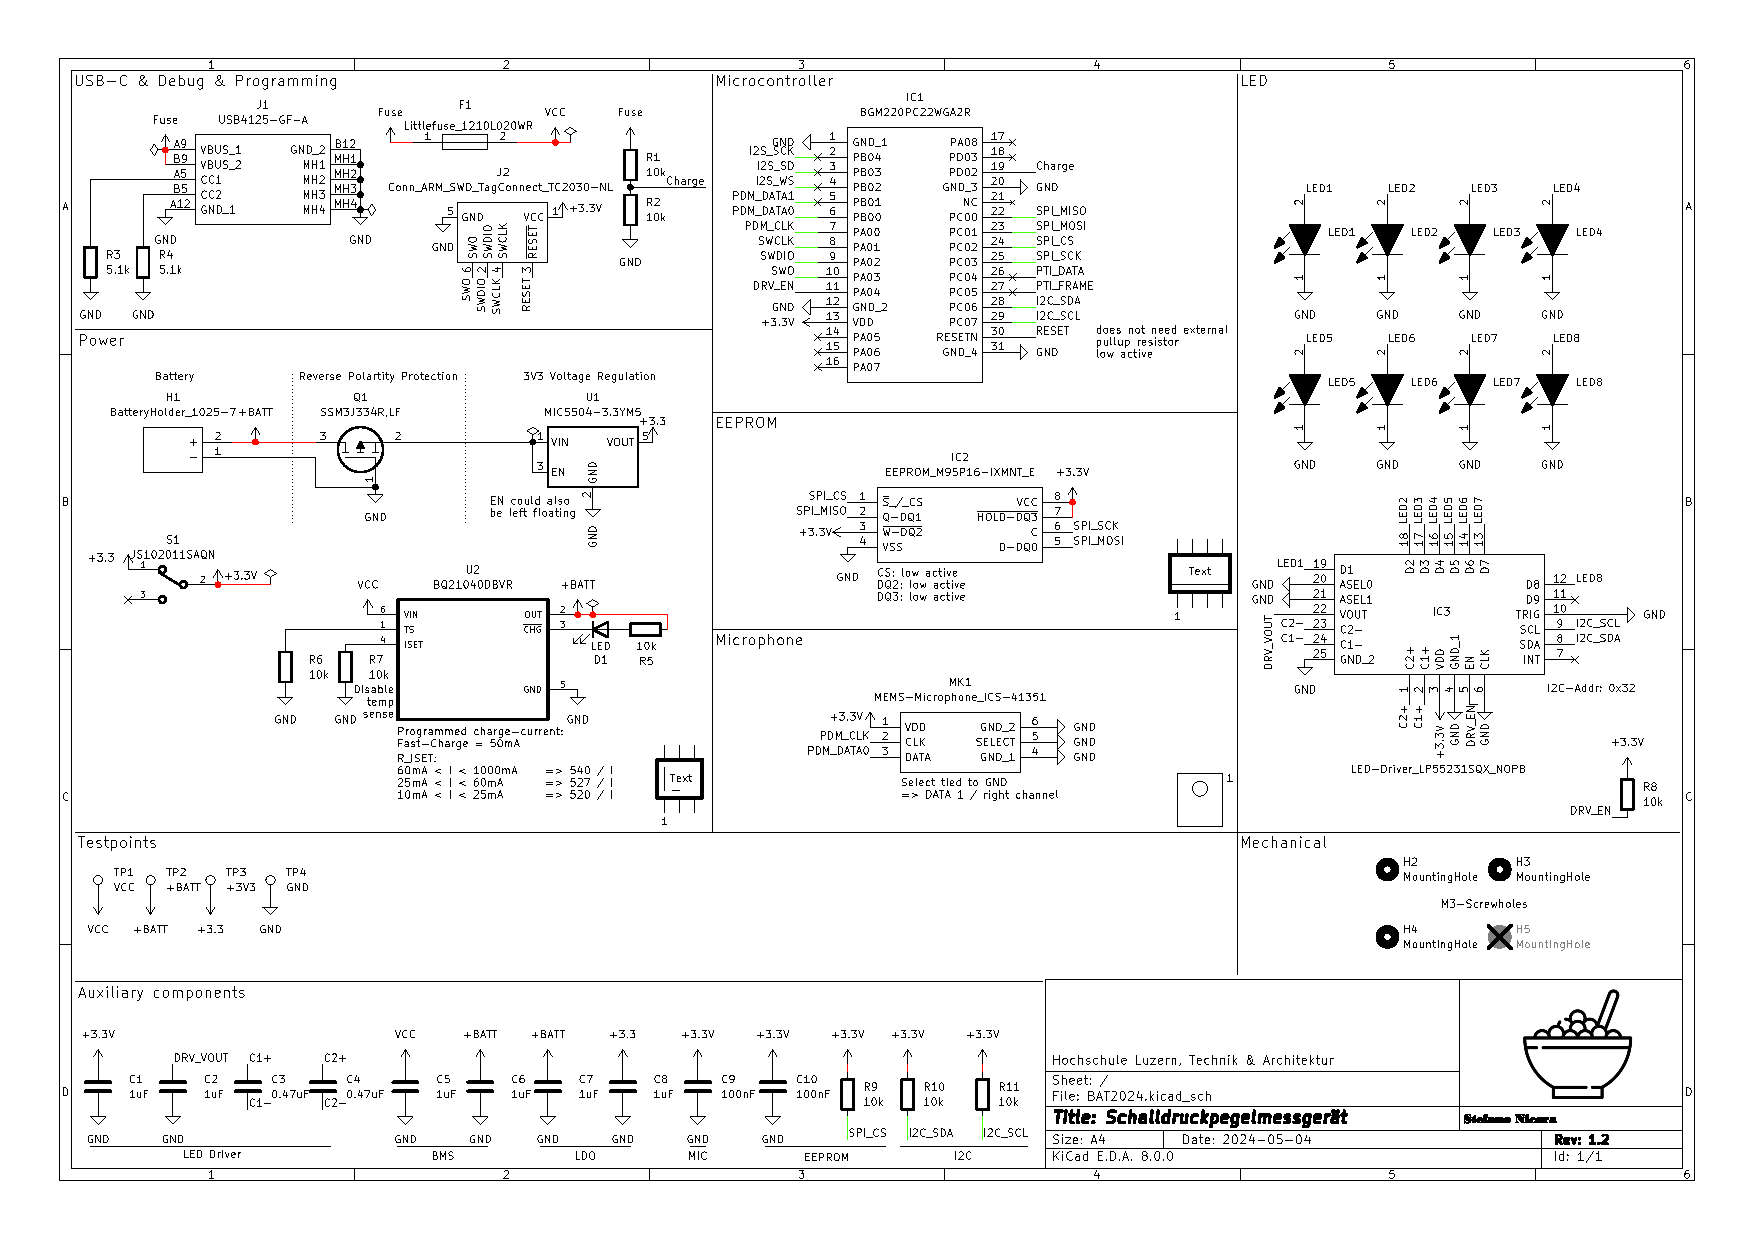
\includepdf[landscape=true, pages={1},scale=0.65]{images/BAT_Schematic_V1-2.pdf}
	\end{minipage}
	
	\newpage
	\subsection*{Software} \label{Anhang:Software}
	\begin{figure}[H]
		\centering
		
\includegraphics[width=1\linewidth]{images/BAT_QR-Code_Github-Repo}
		\label{fig:batqr-codegithub-repo}
	\end{figure}
	https://github.com/Froster2406/BAT2024 \\ \\ \\
	Oder alternativ im digitalen Anhang unter:\\
	$$Entwicklung/Software/custom$$
	
	\newpage
	\subsection*{Aufgabenstellung}\label{Anhang:Aufgabenstellung}
	\begin{minipage}[b]{\textwidth}
		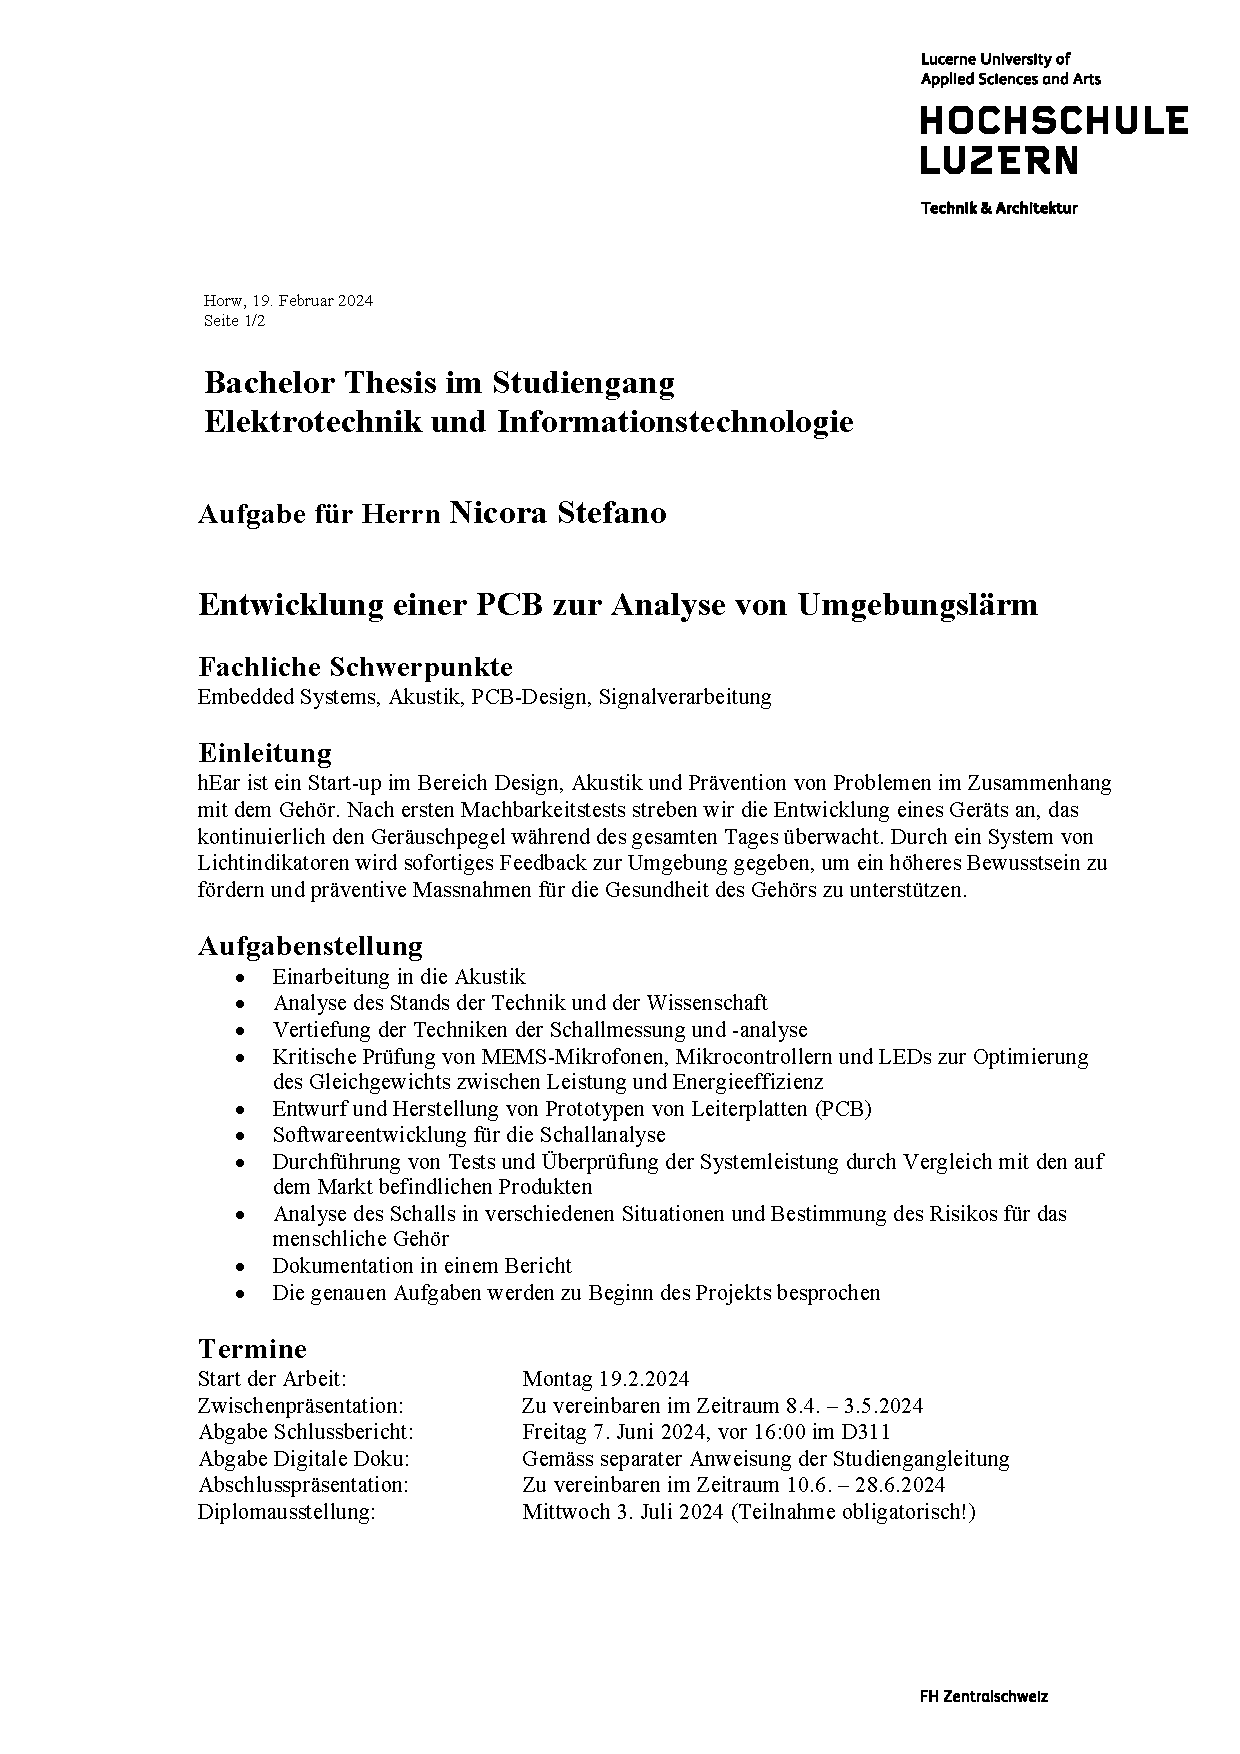
\includepdf[pages={1}, scale=0.9, pagecommand={}]{images/Aufgabenstellung.pdf}
	\end{minipage}
	\newpage
	\begin{minipage}[b]{\textwidth}
		\includepdf[pages={2}, scale=0.9, pagecommand={}]{images/Aufgabenstellung.pdf}
	\end{minipage}
	
	\newpage
	\subsection*{Anforderungskatalog}\label{Anhang:Anforderungskatalog}
	\begin{figure}[H]
		\centering
		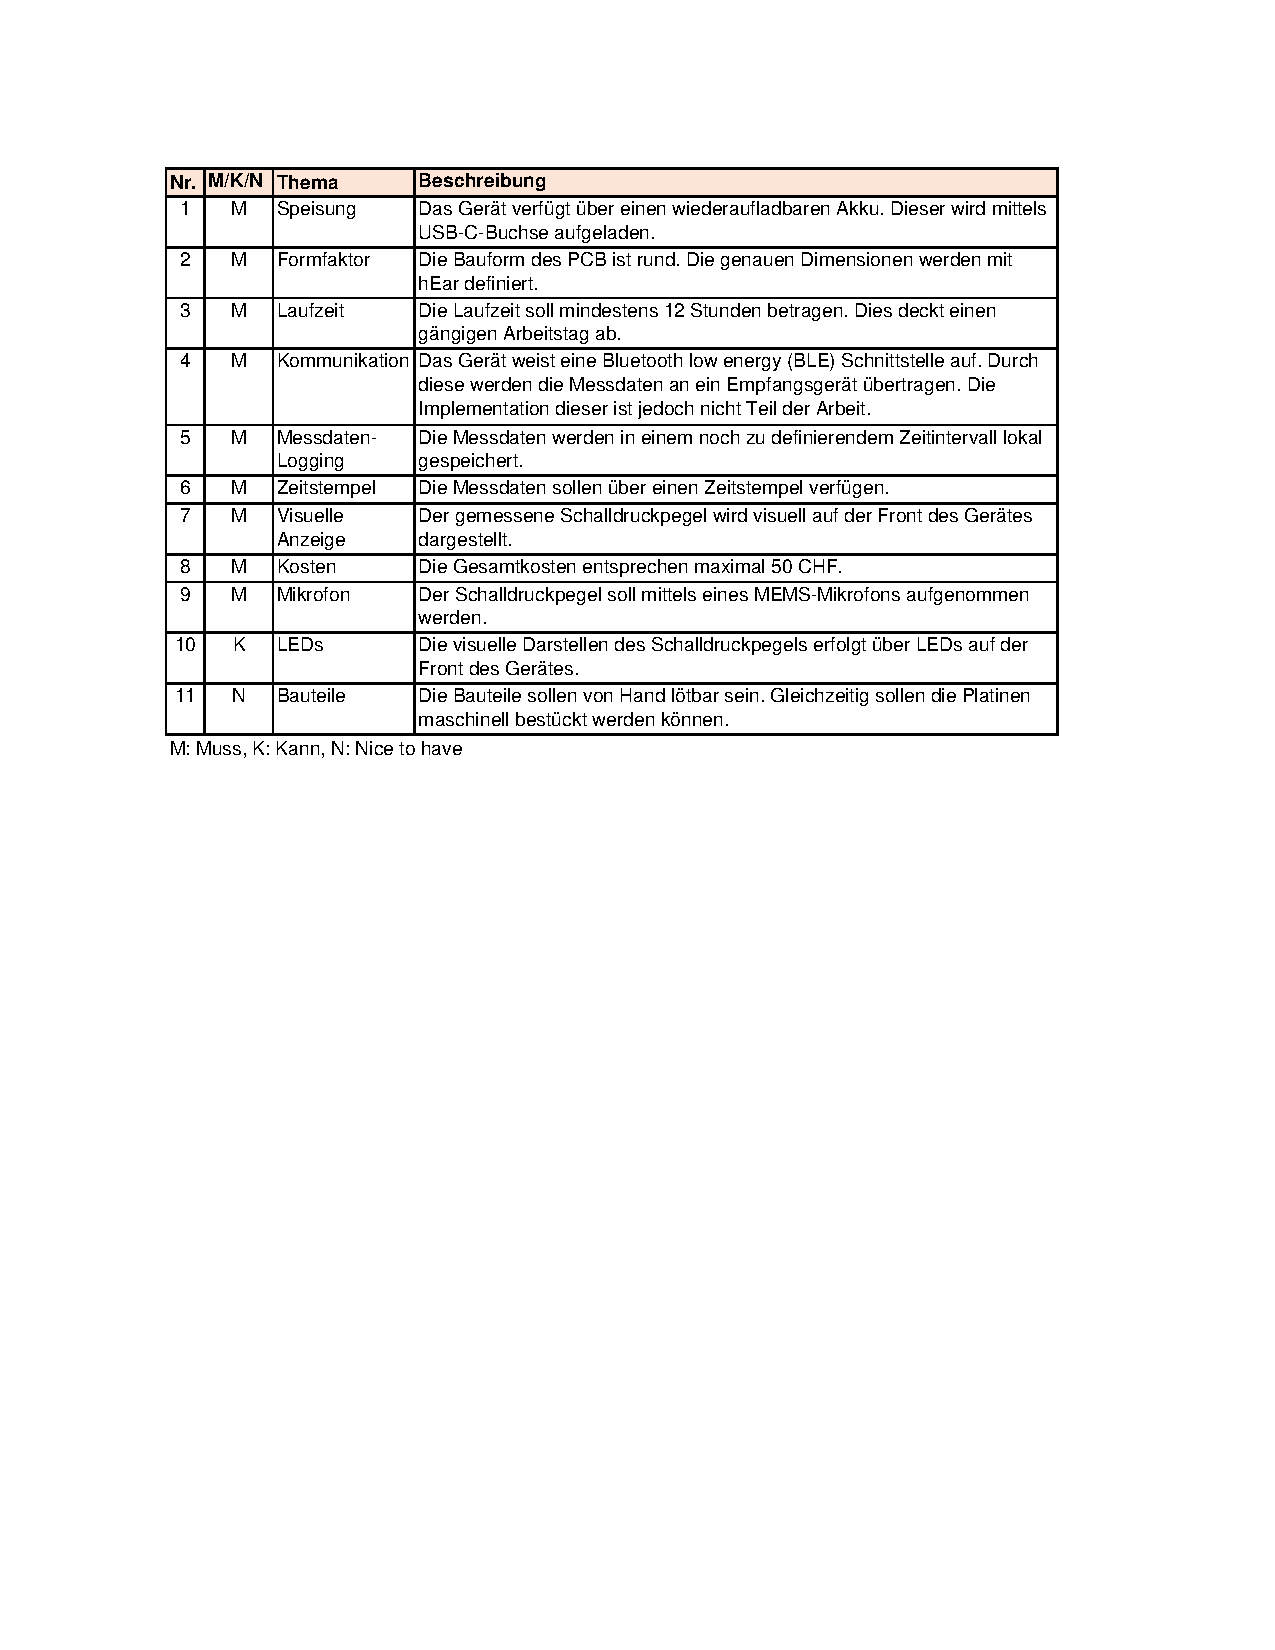
\includegraphics[trim= 2.5cm 5cm 0cm 3.5cm, width=1.2\linewidth]{images/BAT_Anforderungskatalog}
	\end{figure}
	
	\newpage
	\subsection*{Risikoanalyse}\label{Anhang:Risikoanalyse}
		\begin{minipage}[b]{\textwidth}
		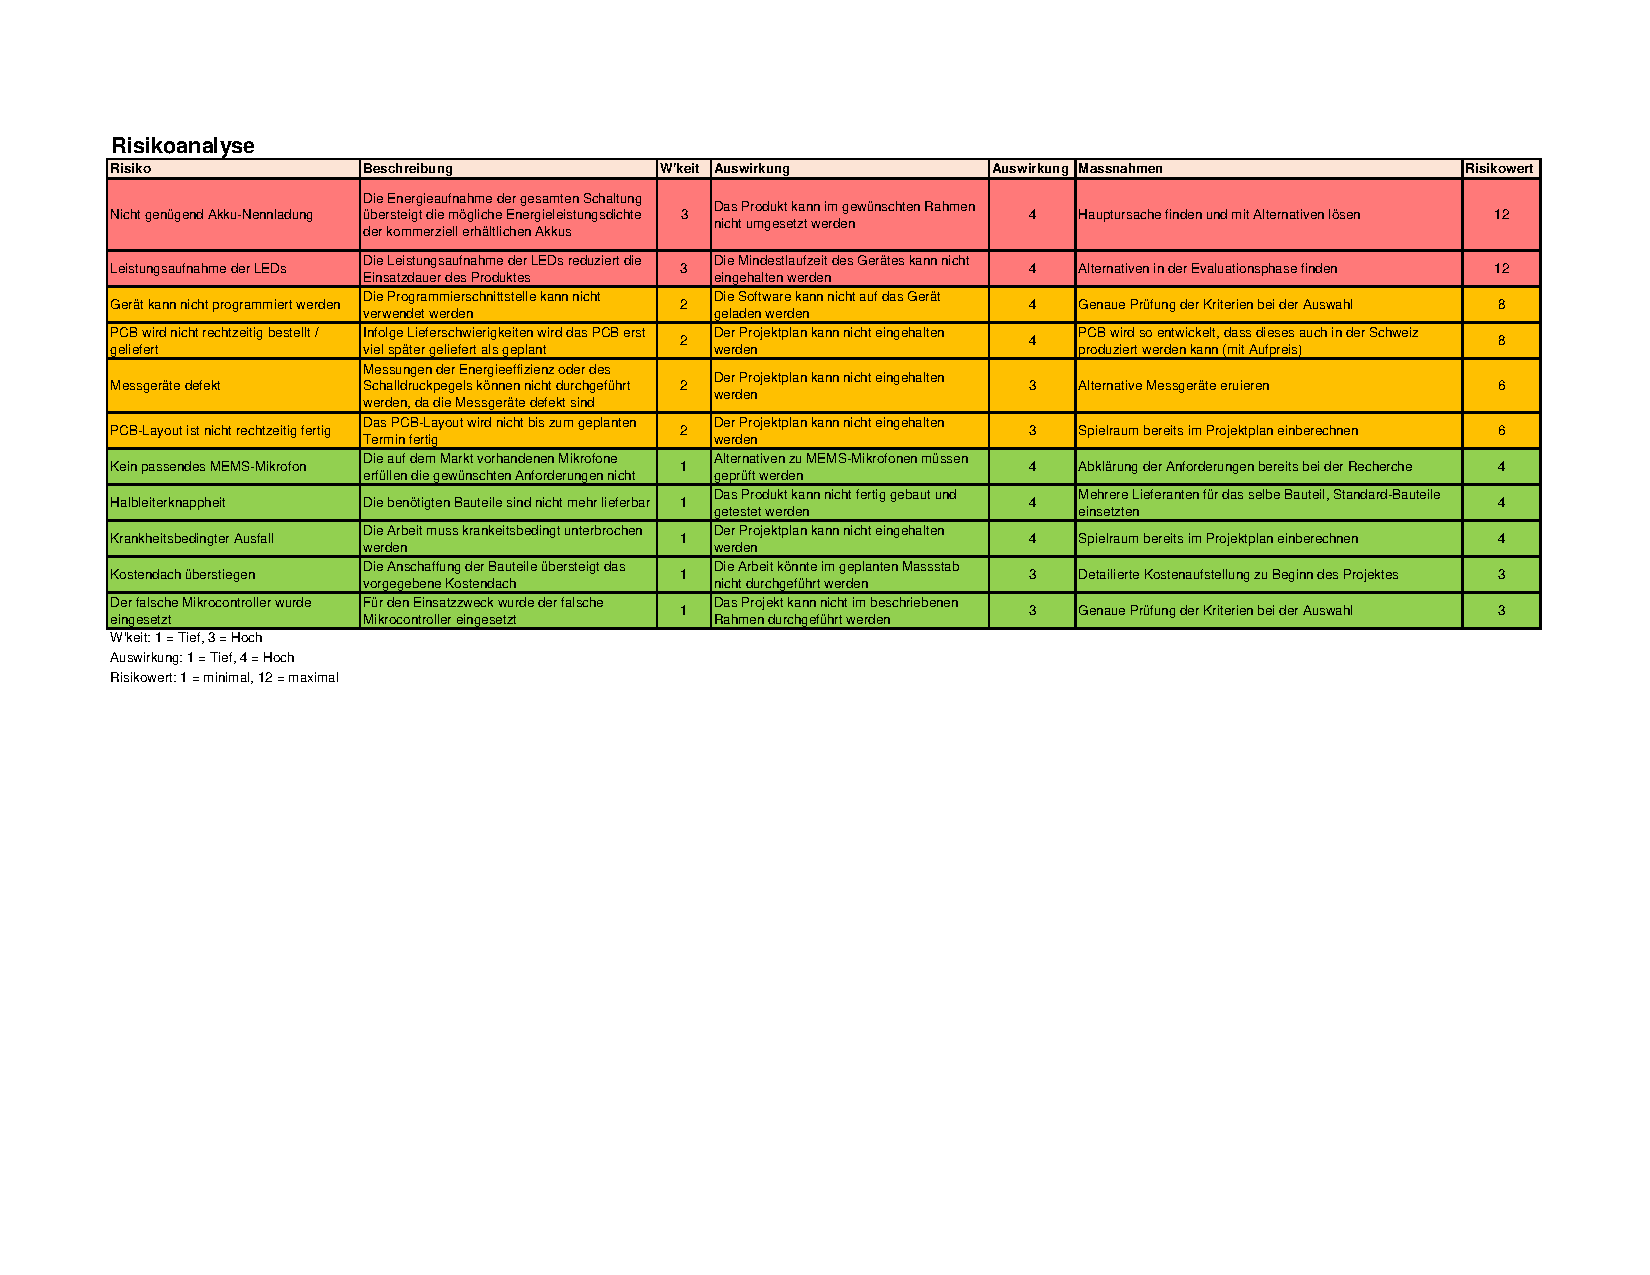
\includepdf[landscape=true, pages={1},scale=0.7, pagecommand={}]{images/BAT_Risikoanalyse.pdf}
	\end{minipage}
	
	\newpage
	\subsection*{Zeitplan}\label{Anhang:Zeitplan}
	\begin{minipage}[b]{\textwidth}
		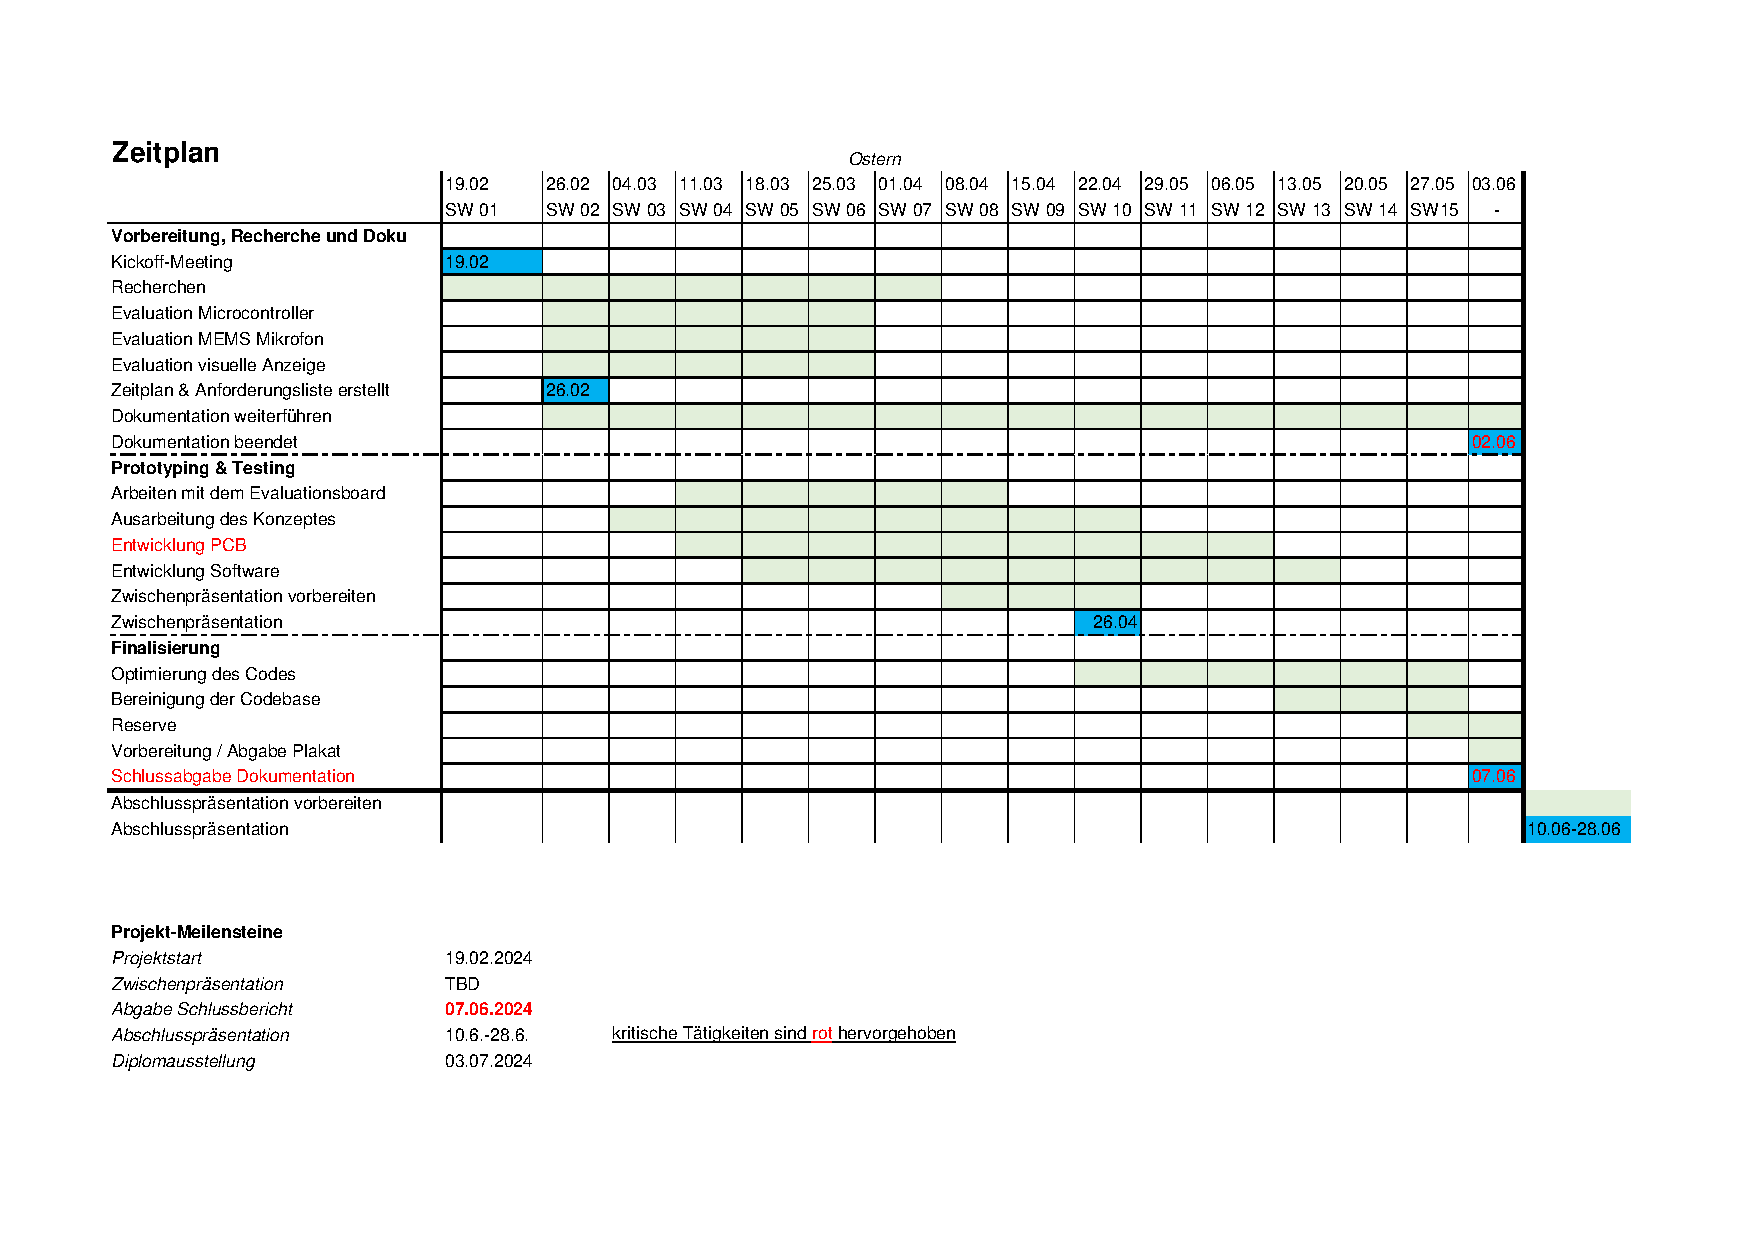
\includepdf[landscape=true, pages={1},scale=0.8, pagecommand={}]{images/BAT_Zeitplan_V2.pdf}
	\end{minipage}

	\newpage
	\subsection*{Journal}
	\begin{table}[H]
		\centering
		\begin{tabular}{|l|p{0.7\textwidth}|l|}
			\hline
			\textbf{Wann} & \textbf{Beschreibung} & \textbf{Zeit (h)} \\ \hline
			17.02.2024 & Ordnerstruktur aufsetzten, Recherche & 4 \\ \hline
			18.02.2024 & Einrichtung Git, Vorbereitung Dokumente & 3 \\ \hline
			19.02.2024 & KickOff, Recherche & 6 \\ \hline
			20.02.2024 & Recherche Mikrocontroller, Vorbereitung Dokumente & 5 \\ \hline
			21.02.2024 & Recherche Mikrocontroller und LEDs, Leistungsaufnahme & 9 \\ \hline
			25.02.2024 & Technologierecherche, Zeitplan, Risikoanalyse, Anforderungskatalog & 7 \\ \hline
			26.02.2024 & Sitzung 2, Technologierecherche, Planung & 6 \\ \hline
			27.02.2024 & Dokumentationsbeginn, Technologierechereche & 5 \\ \hline
			02.03.2024 & Vergleich Mikrokontroller & 4 \\ \hline
			03.03.2024 & Recherche Flash-Chips, BLE vs Bluetooth Classic & 5 \\ \hline
			04.03.2024 & Vergleich LEDs, MEMS-Mikrofon; Einarbeitung LaTeX \& Zotero & 8 \\ \hline
			05.03.2024 & Sitzung, Bauteilbestellung, Einrichten KiCad & 6 \\ \hline
			06.03.2024 & PCB-Schema zeichnen & 3 \\ \hline
			09.03.2024 & PCB-Schema V1.0 beenden & 3 \\ \hline
			10.03.2024 & PCB-Layout Planung & 4 \\ \hline
			11.03.2024 & PCB-Routing, Einrichtung Simplicity Studio & 8 \\ \hline
			12.03.2024 & Sitzung, PCB-Routing & 4 \\ \hline
			13.03.2024 & PCB-Routing & 5 \\ \hline
			15.03.2024 & PCB-Routing, Besprechung Christoph Zumbühl & 3 \\ \hline
			16.03.2024 & Bestückung Breakout-Board, Doku weiterführen & 5 \\ \hline
			17.03.2024 & Erste Tests mit DIE und Mikrofon & 3 \\ \hline
			18.03.2024 & Einarbeitung Filterdesign, RTC, Korrespondenz & 7 \\ \hline
			19.03.2024 & Sitzung, Softwareentwicklung & 6 \\ \hline
			23.03.2024 & Softwareentwicklung SPI & 3 \\ \hline
			24.03.2024 & Softwareentwicklung I2C, Dokumentation & 4 \\ \hline
			25.03.2024 & Softwareentwicklung, Testing & 7 \\ \hline
			26.03.2024 & Sitzung, Softwareentwicklung I2C & 7 \\ \hline
			27.03.2024 & Softwareentwicklung I2C & 7 \\ \hline
			28.03.2024 & Softwareentwicklung I2C, PCB Redesign & 8 \\ \hline
			29.03.2024 & Einarbeitung PDM & 6 \\ \hline
			30.03.2024 & Einarbeitung PDM & 6 \\ \hline
		\end{tabular}
	\end{table}
	\begin{table}[H]
		\centering
		\begin{tabular}{|l|p{0.7\textwidth}|l|}
			\hline
			\textbf{Wann} & \textbf{Beschreibung} & \textbf{Zeit (h)} \\ \hline
			01.04.2024 & Softwareentwicklung PDM, Dokumentation & 7 \\ \hline
			02.04.2024 & Softwareentwicklung Timer, RTC & 7 \\ \hline
			03.04.2024 & Dokumentation & 6 \\ \hline
			06.04.2024 & PCB Löten, Fehlersuche, Anpassungen & 8 \\ \hline
			08.04.2024 & PCB Programmieren, Fehlersuche & 4 \\ \hline
			09.04.2024 & Sitzung, Besprechung Filter Jürgen Wassner & 5 \\ \hline
			10.04.2024 & Filterdesign, Besprechung Filter Pascal Jund & 6 \\ \hline
			13.04.2024 & Filterdesign & 2 \\ \hline
			14.04.2024 & Filterdesign, PPP vorbereiten, Dokumentation & 4 \\ \hline
			15.04.2024 & PDM-Fehlersuche, Dokumentation & 7 \\ \hline
			16.04.2024 & Sitzung, PDM-Fehlersuche, Dokumentation & 7 \\ \hline
			17.04.2024 & PDM-Fehlersuche, Dokumentation & 6 \\ \hline
			20.04.2024 & PDM Implementation blocking, PCB revision V1-3 & 8 \\ \hline
			21.04.2024 & Dokumentation weiterführen & 5 \\ \hline
			22.04.2024 & Softwareentwicklung, PDM Fehlersuche & 8 \\ \hline
			23.04.2024 & Sitzung Sophie, Softwareentwicklung & 7 \\ \hline
			24.04.2024 & Softwareentwicklung & 7 \\ \hline
			26.04.2024 & Präsentation inkl. Vorbereitung & 3 \\ \hline
			27.04.2024 & Evaluation alternative RTC $->$ keine & 4 \\ \hline
			28.04.2024 & Dokumentation Abschnitt: State of the Art & 2 \\ \hline
			29.04.2024 & Softwareentwicklung, Dokumentation & 7 \\ \hline
			30.04.2024 & Sitzung, Softwareentwicklung, Messungen & 6 \\ \hline
			01.05.2024 & Softwareentwicklung & 4 \\ \hline
			04.05.2024 & Dokumentation weiterführen & 4 \\ \hline
			05.05.2024 & Dokumentation weiterführen & 3 \\ \hline
			06.05.2024 & PCB V1-3 löten, Messungen & 7 \\ \hline
			07.05.2024 & Messungen, Fehlersuche PDM & 6 \\ \hline
			08.05.2024 & Messungen, Fehlersuche PDM & 4 \\ \hline
			09.05.2024 & Fehlersuche PDM & 8 \\ \hline
			11.05.2024 & Fehlersuche PDM & 5 \\ \hline
			12.05.2024 & Messungen, Dokumentation weiterführen & 6 \\ \hline
			13.05.2024 & Messungen, Dokumentation weiterführen & 6 \\ \hline
			14.05.2024 & Sitzung, Dokumentation weiterführen & 6 \\ \hline
			15.05.2024 & Dokumentieren, Fehlersuche & 5 \\ \hline
			18.05.2024 & Fehlersuche IDE & 6 \\ \hline
			19.05.2024 & Fehlersuche IDE, Dokumentation überarbeiten & 7 \\ \hline
		\end{tabular}
	\end{table}
	\begin{table}[H]
		\centering
		\begin{tabular}{|l|p{0.7\textwidth}|l|}
			\hline
			\textbf{Wann} & \textbf{Beschreibung} & \textbf{Zeit [h]} \\ \hline
			20.05.2024 & Messungen beenden, Dokumentation überarbeiten & 6 \\ \hline
			21.05.2024 & Sitzung, Dokumentation weiterführen & 4 \\ \hline
			22.05.2024 & Plakat \& Präsentation vorbereiten & 10 \\ \hline
			~ & \textbf{Optional und nicht mehr Teil der eigentlichen Arbeit} & ~ \\ \hline
			24.05.2024 & Fehlersuche SNR & 4 \\ \hline
			25.05.2024 & Messung SNR mit unterschiedlichen Speisespannungen & 7 \\ \hline
			26.05.2024 & Messung SNR mit unterschiedlichen Startzeiten & 6 \\ \hline
			27.05.2024 & Messung Clock-Jitter & 6 \\ \hline
			28.08.2024 & Einbinden der Messungen in die Dokumentation (Anhang) & 8 \\ \hline
			~ & ~ & ~ \\ \hline
			~ & \textbf{Total} & \textbf{390} \\ \hline
			~ & Total (inkl. optionalem Teil) & 421 \\ \hline
		\end{tabular}
	\end{table}
	
\end{document}